%%
%% This is file `example/bare_thesis.tex',
%% generated with the docstrip utility.
%%
%% The original source files were:
%%
%% install/buptgraduatethesis.dtx  (with options: `bare-thesis')
%% 
%% This file is a part of the example of BUPTGraduateThesis.
%% 

\documentclass[%
  degree=master,%
  classlevel=open,%
  mathfont=mathptmx,%
  dedication=false,%
  chapbib=false,%
  finish=print,%
  driver=xetex]{buptgraduatethesis}

%% 自定义导言区
%% 在这里添加你需要的宏包、自定义命令、环境等
%% \usepackage{...}
%% \DeclareMathOperator{\CT}{H}
%% \DeclareMathOperator{\Cov}{Cov}
\usepackage{algorithmic}
\usepackage{algorithm}
\usepackage{graphicx}
% \usepackage[table,xcdraw]{xcolor}
\def\BUPTThesis{\textsc{BUPT}\-\textsc{Thesis}}

%% 在这里添加图片文件搜索目录
\graphicspath{{../}}
%% 自定义导言区结束

%% 加载缩略语定义
%%
%% This is file `example/metadata.tex',
%% generated with the docstrip utility.
%%
%% The original source files were:
%%
%% install/buptgraduatethesis.dtx  (with options: `metadata')
%% 
%% This file is a part of the example of BUPTGraduateThesis.
%% 

%% 涉密论文保密年限
\classdur{三年}

%% 学号
\studentid{2019110193}

%% 论文题目
\ctitle{面向时延保障的段路由航点选择算法研究}
\etitle{Research on Segment Routing List Generate Algorithm for Network Latency}

%% 申请学位
\cdegree{工学硕士}

%% 院系名称
\cdepartment{信息与通信工程学院}
\edepartment{School of Information and Communication Engineering}

%% 专业名称
\cmajor{信息与通信工程}
\emajor{Information and Communication Engineering}

%% 你的姓名
\cauthor{赖丽蓉}
\eauthor{Lirong Lai}

%% 博士后研究工作报告-分类号
\classnumber{O441.3}

%% 博士后研究工作报告-UDC
\udc{621.396.9}

%% 博士后研究工作报告-学校编号
\schoolserial{147227}

%% 博士后研究工作起始时间
\startdate{2014年10月29日}

%% 博士后研究工作期满时间
\finishdate{2016年4月2日}

%% 你导师的姓名
\csupervisor{刘韵洁}
\esupervisor{Yunjie Liu}

%% 日期自动生成,也可以取消注释下面一行,自行指定日期

%% 中文摘要
\cabstract{%
段路由是一种网络层的路由思想,正在越来越多地应用于网络流量调度中。而随着网络中的业务对时延提出了越来越高的要求,网络需要从各个层面考虑时延保障的效果。本文提出了两种算法,第一种段路由航点生成算法将通过基于软件定义网络控制器的集中式算法实现一种网络拓扑层的段路由策略计算,并得出具有一定程度延迟保证效果的段列表,并通过实验验证得到该算法比只使用带宽信息来生成段路由航点列表对服务请求的时延保障效果好了14.7\%。第二个航点路由算法则是以分布式的为主导思想,通过规划节点时延探测的对象、生成基于差分思想分组的时延矩阵、时延矩阵的更新方式以及段路由航点列表的生成方式最终得到具有时延保障效果的段路由列表,并且经过实验验证得出结论,在损失一定网络吞吐量的情况下该算法在保障时延需求方面比使用传统最短路径算法的协议好43.9\%。
}

%% 中文关键词,关键词之间用 \kwsep 分割
\ckeywords{软件定义网络 \kwsep 段路由 \kwsep 流量工程 \kwsep 网络时延}

%% 英文摘要
\eabstract{%
Segment Routing is a network layer routing idea that is increasingly being used in network traffic engineering. And as the services in the network put higher and higher demands on the latency, the network needs to consider the effect of latency guarantee from all levels. In this paper, we propose two algorithms, the first of which is a Segment List generation algorithm that uses a centralized algorithm based on a Software Defined Network controller to calculate a Segment Routing policy at the network topology level and derive a Segment List with a certain degree of latency guarantee. The algorithm is experimentally validated to be 14.7\% better than using only bandwidth information to generate a Segment List to guarantee the latency of requests. The second Segment Routing algorithm is based on a distributed approach, which plans the nodes' latency detection objects, generates a latency matrix based on differential grouping, updates the delay matrix, and generates a Segment List to obtain a latency-safe request. The experimental verification concluded that the algorithm is 43.9\% better than the protocol using the traditional shortest path algorithm in terms of securing the delay requirements at a certain loss of network throughput.
}

%% 英文关键词,也用 \kwsep 分割
\ekeywords{%
Software Defined Network \kwsep Segment Routing \kwsep Traffic Engineering \kwsep Network Latency}


\loadglsentries{acronyms}

%% 攻读学位期间发表论文
%% 用 \newcite{<suffix>}{<caption>} 声明不同的论文类型(例如: 期刊论文、会议论文等)。每一个类型的对应的 .bib 文件用 \bibliography<suffix> 命令加载,用 \nocite<suffix> 命令引用。具体请参考 pubs.tex 中的示例
\newcite{jrnl}{期刊论文}
\newcite{conf}{会议论文}
\newcite{patent}{专利}

\begin{document}
%% 声明前置部分
\makefrontmatter

%% 生成主要符号对照表
%%
%% This is file `example/notations.tex',
%% generated with the docstrip utility.
%%
%% The original source files were:
%%
%% install/buptgraduatethesis.dtx  (with options: `notations')
%% 
%% This file is a part of the example of BUPTGraduateThesis.
%% 

\begin{listofnotations}
\item [$(\cdot)^*$] 复共轭
\item [$(\cdot)^{\mathrm T}$] 矩阵转置
\item [$(\cdot)^{\mathrm H}$] 矩阵共轭转置
\item [$\mathbf{X}$] 矩阵或向量
\item [$\mathcal{A}$] 集合
\item [$\mathcal{A}\times\mathcal{B}$]
  集合 $\mathcal{A}$ 与集合 $\mathcal{B}$ 的 Cartesian 积,即 $\mathcal{A}\times\mathcal{B}=\{(a,b):a\in\mathcal{A},b\in\mathcal{B}\}$
\end{listofnotations}


%% 主体部分
\mainmatter
%% 用\include{}命令引用各章.tex文件
%%
%% This is file `example/ch_intro.tex',
%% generated with the docstrip utility.
%%
%% The original source files were:
%%
%% install/buptgraduatethesis.dtx  (with options: `ch-intro')
%% 
%% This file is a part of the example of BUPTGraduateThesis.
%% 

\chapter{绪论}
\section{研究背景及其意义}

1. 段路由的研究背景

\gls*{SDN} 场景下,控制器作为网络设备的管控面可以获得网络全局拓扑信息,但是网络流量全部使用软件定义网络机制进行调控,往往会缺少一些灵活性和时效性。例如网络流量工程全部使用 \gls*{MPLS} 是当前业界依旧常用的流量工程调度方案,其使用的初衷是使用标签替代交换机IP进行快速转发,多协议标签交换按照拓扑用控制驱动而非更传统的流量驱动,这样就更加优化了工作原理。存储资源稀缺对标签进行匹配并分配出端口的操作可以不上送CPU就能够完成,因此降低了交换机对报文的处理查表时延,提高了转发效率。但是标签的分发和通告需要 \gls*{IGP} 或 \gls*{OSPF} 进行传输。除此以外,多协议标签交换在工作时,每个下一跳都是确定的,即网络中完整的一条隧道都需要给该多协议标签交换策略下的流量预留出来,这就需要作为流量工程的 \gls*{RSVP} 扩展的 \gls*{RSVP-TE} 在IP网络上预留资源,同时还需要 \gls*{LDP} 用于分配标签。IP网络终端运行的应用程序可以基于资源预留机制向其他节点表明终端所要接收的数据包流的性质(如带宽,抖动,最大突发量等),可以使边缘计算多协议标签交换路径的装置依照需求进行流量转发路径分配。但是当前的多协议标签交换部署方式存在一些弊端:一是基于流量工程扩展的资源预留协议的操作开销通常很高;二是IP网络原本可以使用 \gls*{ECMP} 做到原生的负载均衡,但多协议标签交换作为显式源路由,将路由路径的标签全部封装在报文头,使得每一跳之间无法进行IP网络原生的多路径负载均衡。

\gls*{SR} 提供了一种新的流量调度思想,不同于源路由规划好每一跳的路径,段路由只在若干跳的范围规划一个目的标签,使得段路由报文头的标签栈只用很少的标签就可以指导网络流量转发,这可以看作是软件定义网络控制器对网络流量的处理模式进行编程,段路由的标签栈就相当于编程的代码,由此达到对网络数据包进行操作的网络编程目的。

但是段路由标签栈需要分配怎样的标签需要具有全局视角的控制平面来决定,可以通过操作员的经验进行配置,也可以在软件定义网络场景下由控制器进行计算分配。目前常用的标签栈计算方式都是基于带宽的,而在业务对时延越来敏感的大环境下,就需要考虑使用时延作为指导标签生成的元素,即在段路由代表的网络层对时延进行一定程度的保障。因此本文将讨论基于软件定义网络控制器全局视角计算具有保障流量时延效果最好的段路由标签栈生成算法。

2. 时延研究背景

近年来学术界和产业界也在越来越多得关注时延带来的问题,其内在的驱动力主要是时延敏感的业务正在蓬勃发展,随着线上办公、线上会议的普及;元宇宙概念的兴起带来增强现实/虚拟现实/实时视频等技术进一步发展;以及物联网车联网概念下对时延苛刻的要求,越来越多的高 \gls*{SLA} 业务对时延的要求明显增强。因此在网络 \gls*{OSI} 模型中的各个层级都开始对时延保障进行探索。

网络中的时延主要分为节点处理时延(Nodal Processing Delay)、排队时延(Queuing Delay)、传输时延(Transmission Delay)、传播时延(Propagation)。而这些时延累加起来是节点间通信总时延(Total Nodal Delay)。实际上节点处理时延往往是微秒级别可以忽略不计;传输时延由光信号在光纤中传播产生,本身引起的时延很小且是客观存在无法进一步优化的时延;传输时延指的是在队列中,当分组在链路上等待传输时,它经受排队时延。一个特定分组的排队时延将取决于先期到达的、正在排队等待向链路传输的分组的数量。如果该队列是空的,并且当前没有其他分组在传输,则该分组的排队时延为0。另一方面,如果流量很大,并且许多其他分组也在等待传输,该排队时延将很大。到达组的分组数量是到达该队列的流量强度和性质的函数。实际的排队时延通常在毫秒到微秒级。

为了优化排队时延,数据链路层上 \gls*{TSN} 正在引起很多研究人员的关注。时延敏感网络旨在保证时延敏感业务流量的服务质量,实现低时延、低抖动和零丢包率的高可用网络。其主要的实现方式就是着眼于发送功率,用排队论、博弈论的思想确定一个合适的信息发送功率,对发送信号进行整形,从发送源头上规避可能出现的排队问题,最终使得业务流量实现超低时延和零丢包,实际上就是使得排队时延降为零,使得网络中只存在客观的处理时延,而这种时延是可预期可计算的。

传输层由于有TCP这种建立端到端链接的协议,对时延更为关注,也更适合参考时延对拥塞控制算法做出调整,例如在Swift中,通过使用 \gls*{AIMD} 的方式来实现端到端的延迟控制,并在极端拥塞的情况下调整步调,通过精确的 \gls*{RTT} 测量并仔细考虑延迟目标。又如 \gls*{HPCC} 利用 \gls*{INT} 来获取精确的链路负载信息并精确控制流量。通过解决拥塞期间延迟的带内遥测信息和对带内遥测信息的过度反应等难题,使得高精度拥塞控制可以迅速收敛以利用空闲带宽,同时避免拥塞,并且可以保持接近零的网络内队列以实现超低延迟。

3. 段路由对时延支持的研究意义

在网络各个层面都开始尝试支持时延保障的情况下,网络层因为其尽全力交付的特性而难以在端到端实验上作出保证,通常和业务相关的需求都由传输层协议完成,网络层的研究方向里只有流量调度可以为服务质量提供一些保障,而段路由正是流量调度的一种新型方法,由于其灵活性已经被网络设备商广泛支持,也被网络运营商广泛使用,最新的Linux内核协议栈也开始支持段路由。

流量调度中的服务质量需求是多种多样的,目前比较常见的有最小化网络能耗、优化拥塞和最小化被拒绝请求的数量,可见最小化流量时延是一个研究还比较缺乏的领域,因此本文将最小化流量时延作为流量工程优化的目的,以段路由为主要实现方式进行段路有航点列表算法设计,这对充实在各个网络分层中对时延需求进行保障具有一定意义。

\section{国内外研究现状}

本节将简要回顾域内流量调度算法的相关研究以及域内流量调度算法在传统IP网络、完全部署段路由的网络和部分部署段路由的网络中使用的机制,即 IP-TE(OSPF-TE)、SR-TE 和混合SR-TE。

在传统的IP网络中,每条链路都被分配了一个权重(即链路成本),不同的链路权重设置会导致不同的转发路径。多商品流(Multi-commodity Flow, MCF)问题是一个经典的优化问题。研究[11]在路由优化和流量工程中应用机器学习(Machine leaning, ML)是新趋势。机器学习算法可以从过去的网络状态中学习流量发生规律,并为未来的网络状态生成合适的路由配置。与启发式算法相比,机器学习具有更具适应性的视角,而不是依赖于人为确定的启发式方法。监督学习(Supervised learning, SL)和强化学习(Reinforcement learning, RL)是已经应用于 流量工程的机器学习的两个分支。监督学习必须从标记的训练数据中学习,这在流量工程领域很难获得。但是,强化学习是从网络环境中学习,而不是通过动作和奖励与网络迭代交互,而不是预先收集的训练数据,因此更适合流量工程。在[16]中,作者比较了两种机器学习方法:一是使用监督学习来预测即将到来的流量矩阵并根据预测的流量矩阵来优化路由;二是使用强化学习学习从历史流量矩阵到路由配置的较好的映射。他们的工作表明,强化学习在路由优化方面比监督学习更有前景。研究[17]使用深度强化学习(Deep reinforcement learning, DRL)和深度确定性策略梯度(Deep Deterministic Policy Gradient Algorithms, DDPG)[18]仅通过设置IP网络中的链路权重,就可以一定程度上优化最小化网络时延。研究[19]则是提出了一种基于深度确定性策略梯度的改进算法,并使用它来决定预定义转发路径上的分流比,而无需指定网络场景。这些研究仅将机器学习尤其是强化学习应用于具有基本决策变量和容易获得奖励的非常简单的网络场景。

除了使用机器学习优化流量工程的计算结果,段路由节点与非段路由节点如何共存保障网络架构平滑过渡也是一个常见的研究重点。在研究[20]中提到。段路由网络中的一个数据包依次通过一系列段路由,段路由列表(Segment list, SL)由入口路由器确定并封装在数据包头中。段列表中的段数称为段列表深度(Segment list deep, SLD)。目前对段路由流量工程的研究主要可以分为两大类:一是建立段路由的网络模型;二是只关注段路由的路径编码问题。在考虑段路由的情况下构建模型时,一些研究利用了适用于大规模网络的启发式方法。哈特等人在[7]提出了一个集中式优化器DEFO,它将以北向接口语言表达的高级目标转换为兼容的网络配置。他们使用本地搜索来搜索最合适的段路由航点列表。在[21]中,作者专注于段路由网络中转发路径的快速重新路由。他们使用预处理、移动预过滤和累积树来加速本地搜索。仍有许多研究使用线性规划(Line programming, LP)解决段路由流量工程问题。这些研究将问题形成为线性规划公式,并使用线性规划求解器进行求解。研究[22]提出了一种没有使用等价多路径路由的路由流量工程算法。在研究[23]中,作者提出了一种2-段路由的方法,该方法将每个流的最大段路由列表深度限制为2,并确定离线和在线情况下分段路由的最佳参数。在[24]中,作者分析了真实世界的交通并扩展了2-段路由公式以最小化非最短路径隧道的数量。他们还评估了3-段路由和4-段路由的流量工程能力,并表明它们非常耗时,因此较长的段路由深度是不值得提倡的。在[25]中,作者研究了基于软件定义网络的广域网中的段路由流量工程,并证明了一般的段路由策略生成问题是一个NP-hard问题。

段路由的路径编码问题旨在将预先计算的流量工程路径编码为一组段列表,同时最小化它们的大小。现有研究仅考虑全段路由节点网络中的路径编码问题。一些研究将路径分解为几个子路径并分别对它们进行编码 [26]、[27]。其他人用辅助图表示转发路径并解决其上的线性规划问题[28],[29]。

目前,基于混合段路由网络的流量工程还处于起步阶段,相关工作很少。在研究[2]中提出了一种在考虑流量工程的同时将段路由增量部署到运营商网络的策略。作者假设支持段路由功能的节点构成分段路由域(Segment routing domain, SRD),这限制了入口段路由节点和出口段路由节点之间路径上的所有节点都必须支持段路由。分段路由域的部署方式适用于基于多协议标签交换的段路由(SR-MPLS)。但是由于基于多协议标签交换的段路由的特性,[2] 不能使用段路由节点段跨不同分段路由域路由流,否则数据包将被非段路由节点丢弃。并且每个分段路由域必须至少有两个段路由节点才能在其内部使用段路由节点。因此,虽然可以通过设置分段路由域数量和段路由数量相等来获得分散部署的IP和段路由共存的混合网络,但它不能使用段路由节点段,所以它不能很好地运作。研究[2]采用默认的开放最短路径优先协议链路权重并使用混合整数线性规划(Mixed-integer linear programming, MILP)优化框架来确定最佳分段路由域构成和流量路径。但是,默认链路权重通常设置为与链路容量成反比的现象可能不适用于段路由。由于分段路由域限制和链路权重设置不当,需要50\%以上的节点升级为段路由节点,才能获得与全段路由网络相当的最大链路利用率。这些工作的主要特点如下:第一它们只在混合段路由网络中优化具有段路由能力的节点的流量路径和位置,而链路权重是固定不变的;第二是所有网络节点都基于完全部署的段路由网络或混合 段路由网络,其中段路由节点部署为分段路由域。这些工作为解决网络过渡阶段混合部署的问题提供了思路。

\section{论文主要结构}

本论文将从段路由的时延保障节点选择,以及基于段路由协议标签列表的时延保障方案的研究点展开。
首先在第一章对时延研究背景和短路有研究背景和现状进行梳理,阐述保障时延的段路由需要解决的问题和面临的挑战,分析保障时延的段路由的意义和与网络中其他层级技术的相关性,最后给出论文的主要篇章结构安排。

其次在第二章进行相关基础研究的介绍,这将包涵三点,其一是对段路由的一个简单的功能梳理;第二是对时延保障相关的网络技术进行分析,得出对时延保障值得研究的方向总结;第三是对网络中时延信息的获取方案进行梳理,总结使用带内遥测获取时延信息进行控制计算的方案。

然后在第三章将基于集中式控制器全局视角的有点,着重研究了集中式的段路由选择航点的算法,并对问题进行模型建立、算法目的分析、算法实现以及基于时延选择段路由航点算法的实验进行测量分析,最终证明在使用集中式控制器进行计算段路由航点列表时将时延因素考虑进来是有益于服务流量时延保障需求的。

在第四章中将扩大网络的规模,因此会从分布式的角度为段路由选择航点列表,本章算法的主要优化目的有:降低时延探测流量的比重,降低段路由跳数对网络吞吐量的影响,在合适的范围保障业务流量的端到端时延。本章参考里边界网关协议相关协议的设计细节,将惩罚值和节点聚合引入分布式段路由节点计算的核心数据结构。并对本章提出的算法进行仿真验证,最终证明该方案对于分布式的时延信息传播既有一定的效果。

最后在第五章对整个论文的工作做一总结并且计划未来在工作中继续研究的方向。

\section{课题来源}
本课题研究主要来源于以下项目的支持:

1)国家重点研发计划:支持高级语言编程的SDN控制系统研究(2020YFB1804603);

2)国家重点实验室课题:基于软件定义的天地一体化网络架构(NST20200104)。

%% 本章参考文献
\ifx\usechapbib\empty
\nocite{BSTcontrol}
\setcounter{NAT@ctr}{0}
\bibliographystyle{buptgraduatethesis}
\bibliography{bare_thesis}
\fi

%%
%% This is file `example/ch_concln.tex',
%% generated with the docstrip utility.
%%
%% The original source files were:
%%
%% install/buptgraduatethesis.dtx  (with options: `ch-concln')
%% 
%% This file is a part of the example of BUPTGraduateThesis.
%% 

\chapter{相关研究基础}
% 脚注使用带圈数字的表示方法,此处为示例 1\footnote{测试脚注一} 和示例 2\footnote{测试脚注二}。

% 参考文献可以使用\cite{BUPT_Thesis_Format_2014}和\onlinecite{BUPT_Thesis_Format_2004}的表示方法。

\section{段路由}

\subsection{段路由发展历史}

在开放系统互连模型网络架构中,网络层的核心协议IP协议只提供尽全力交付的服务,是无连接、不可靠的,因此网络流量服务的可靠性通常由传输层协议 \gls*{TCP} 来完成。而对于IP层的路由协议来说,如何评估网络的性能以及如何对网络性能进行优化依然是需要考虑的问题。虽然 \gls*{OSPF} 和 \gls*{IS-IS} 等协议定义了路由器之间如何通信以及何时更新链路权重等信息,但它们并不能对网络性能做出评估。为此,一个IP网络层的关键问题就是如何预测或估计网络中的流量状态,以及IP网络如何实现一些业务可能感兴趣的网络性能度量。这就产生了网络流量工程,流量工程是为了处理IP网络的性能评估和性能优化问题。流量工程包括了各种应用于网络流量的测量、表征、建模和控制的技术和科学原理。而对于使用网络流量工程的网络工程师来说,流量工程的目标就是通过合适的技术手段获得适当的链路权重来使业务的流量运行在符合其带宽、抖动、时延、丢包率等 \gls*{QoS} 需求的路由路径上。

自从 \gls*{MPLS} 诞生以来,使用 \gls*{MPLS} 隧道技术实现流量工程就是一种最常用的流量工程方法。甚至一提到流量工程,工程师们通常都会着眼 \gls*{MPLS} 来实现流量工程。 \gls*{MPLS} 流量工程需要网络运营商为每条链路分配带宽值。分配的带宽通常等于链路的物理带宽。 \gls*{MPLS} 流量工程还允许为每个 \gls*{MPLS} 隧道分配带宽值。该值通常等于测量的隧道承载的流量。因为链路的分配带宽值和 \gls*{LSP} 由 \gls*{RSVP} 发出信号,这些带宽值通常称为链路和隧道的资源预留协议带宽。在将隧道放置到网络上时, \gls*{MPLS} 流量工程将确保在任何链路上,通过该链路的所有隧道的带宽总和小于该链路的带宽。从概念上讲,这可确保每条链路的带宽都超过所需的带宽,从而防止拥塞。

\gls*{MPLS} 是很成熟的流量工程协议,但是它的问题在于两点,一个是 \gls*{MPLS} 需要规划好一条流量每一跳的目的地址,使得流量十分精确地按照预期的路线传输,这就使得 \gls*{MPLS} 不能很好地绕过网络中随机出现的链路故障,并且完全架空了IP网络天生支持的 \gls*{ECMP} 等负载均衡方式,使得流量工程强依赖于对链路进行精确计算的管理控制设备,缺少自愈的可能;第二点是在于 \gls*{RSVP} 为了对网络带宽作出精确的估算,相当占据网络中的各种资源,尤其是当网络规模日益扩大之后,资源预留协议需要协商的链路及路由器也越来越多, \gls*{RSVP} 的过于冗杂对网络运行造成了比较大的负担。

因此在2015年,思科提出了段路由技术 \cite{SRARK}。段路由是一种相对较新的流量工程方法,在此之前更常用的流量工程技术。段路由的关键思想是将路由路径分解为分段,以便从宏观上更简单地控制路由路径,从而提高网络利用率。为了与现有网络技术兼容实现平滑过渡,段路由技术在提出伊始就准备了两套数据面,一个是于 \gls*{MPLS} 的段路由,一个是基于IPv6的段路由SRv6。基于 \gls*{MPLS} 的段路由的段标签在本质可以看做是和 \gls*{MPLS} 标签含义相同的属性,路径上的路由器仍然可以使用 \gls*{MPLS} 传统的推送、弹出和交换操作数据包头的段路由报文头。基于 \gls*{MPLS} 的段路由和基于 \gls*{MPLS} 一样有两种基本类型的段标签:节点标签(Node Segment)和邻接标签(Adjacency Segment)。节点段标识路由器节点,节点段的编号在整个分段路由域中是全局唯一的。邻接段代表节点的本地接口。相邻段编号通常仅在本地有意义在每个节点上。由于可以使用相同的标签交换机制,因此可以利用 \gls*{MPLS} 数据平面基本上无需修改即可实现分段路由。除了与已有网络方案无缝过渡外,段标签使用对当前域内路由协议的简单扩展以在整个网络中分发,因此分发标签不再需要 \gls*{LDP} 和 \gls*{RSVP-TE} 。因此,可以显着简化控制平面的协议和流量。此外,段路由与 \gls*{MPLS} 技术不同的是,除了在入口节点上,不需要在分段路由中维护路径状态,因为现在数据包是根据它们携带的分段列表进行路由的。而数据包的修改必须在入口节点完成,因为入口节点需要确定段路由策略并将分段标签添加到数据包中。

一个基本的段路由实现如图2-1所示,入口节点在数据包的IP头上添加一组段路由节点标签,每个标签指向一个段路由节点,这些标签会用作每一段路由中的临时目的地址,沿途的非目的地址交换机就会使用标准最短路径路由算法路由数据包。当数据包从入口到达中间目的地时,中间目的地弹出顶级标签,现在数据包再次沿着最短路径从中间节点路由到下一个段的端点。一个$n$段的段路由路径被称n-段路由($n-segment$)。如果可以允许任意数量的段,段路由就可以衍生使用任意路径,因此在一个路由段数不被限制的n-段路由问题中,在段路由网络中生成段路有航点列表就可以被视为解决多商品流问题。这种灵活性是以增加标签开销和增加网络中的标签处理为代价的。从流量工程的角度来看,远离最短路径路由的大部分好处都可以通过使用两跳来实现。实验研究表明 \cite{SIDLENGTHANALYSIS} \cite{SIDLENGTHPROVE} ,2-段路由的表现几乎与完全不限制段路由长度的解决多商品流问题一样好。因此,本文会关注使用本文提出算法的2-段路由的表现,即其中入口和出口之间的流量只通过一个中间段路由节点。本文中开发的相同技术可以扩展到具有2个以上段的段路由,但是这确实会造成计算量增加代价。除了段路由列表的长度外,在段路由问题中控制平面也起到了很大的作用,因此研究控制平面如何为每个流选择合适的段路由策略才能以最大限度地减少整体网络拥塞也是一个常见的段路由研究方向。

对于段路由研究领域的类别,Ventre \cite{SRSURVEYS} 等的研究提出了一个比较全面的分类方式,它是基于对七个主要研究类别段路有研究领域分类。第一个是监控类,收集所有描述和实现与网络监控活动相关的工具的作品。一些示例包括测量给定输入路线上的端到端延迟或评估交通流量。第二类是流量工程,包括所有提出高级路由策略以优化网络性能的工作。第三类是故障恢复,涵盖在节点/链路故障的情况下提供快速网络恢复的解决方案。由于时间尺度的限制,这一类的工作是基于本地机制的,即不涉及中央控制器。定义的第四类是集中控制架构,包括所有侧重于在底层网络(IP网络、软件定义网络、 \gls*{MPLS} 网络)之上实现集中控制平面的段路由网络实施的论文。在这里我们指出,尽管一些归类为交通工程的工作是基于集中控制的架构,但它们不包括在集中控制的架构中类别。这是因为它们的主要范围仍然是优化流量工程目标(例如减少拥塞或最小化能源消耗)。在路径编码类别中,研究将所有提出旨在将网络路径转换为段路由列表的算法的论文分组。具体来说,研究将通用路径编码算法提供的一系列节点和链接形式的路径作为输入,将在数据包头中推送的段路由编码序列作为输出,以便引导数据包沿着输入路径。第六类是网络编程,包括利用段路由的可编程性特性的解决方案的科学著作,即使用基于服务的段路由编码来定义要在穿过特定段列表的数据包上执行的功能。属于这一类别的作品的一个重要例子包括与服务功能链相关的作品。

\subsection{段路由模型}

首先,段路由的数据平面定义了如何对要应用于数据包的分段序列进行编码,以及分段的转发语义(每个设备应如何基于分段处理数据包)。所描述的段路由操作与用于携带段路由报头信息的实际协议无关。段路由的控制平面定义了段标识符如何在网络设备之间传播,以及如何指示网络设备在流上应用给定的段列表。

1. 段路由数据面

从抽象的角度来看,段路由头包含一个段序列,以及一个指向数据包活动段的指针,是处理数据包的设备需要执行的指令。当活动段被执行后,列表中的下一个段成为活动段。段标签(Segment ID, SID)是段的标识符。根据其类型,段路由编号可以具有域范围的意义,也可以仅对处理它的路由器在本地有意义。

段标签的类型通常有:与节点关联的、路由器分配时需要确保一个域范围的唯一的节点段标签,通常由网络工程师手动完成,或使用中央控制器分配完成;每个路由器将为它的每个 \gls*{IGP} 邻居分配的一个仅本地有效的邻接段标签;标记网络中可以提供指定服务节点的服务段标签(Service SID),各个段标签的类型及其用途如图2-1所示。

\begin{figure}[htbp]
\setlength{\abovecaptionskip}{15pt plus 3pt minus 2pt}
\centerline{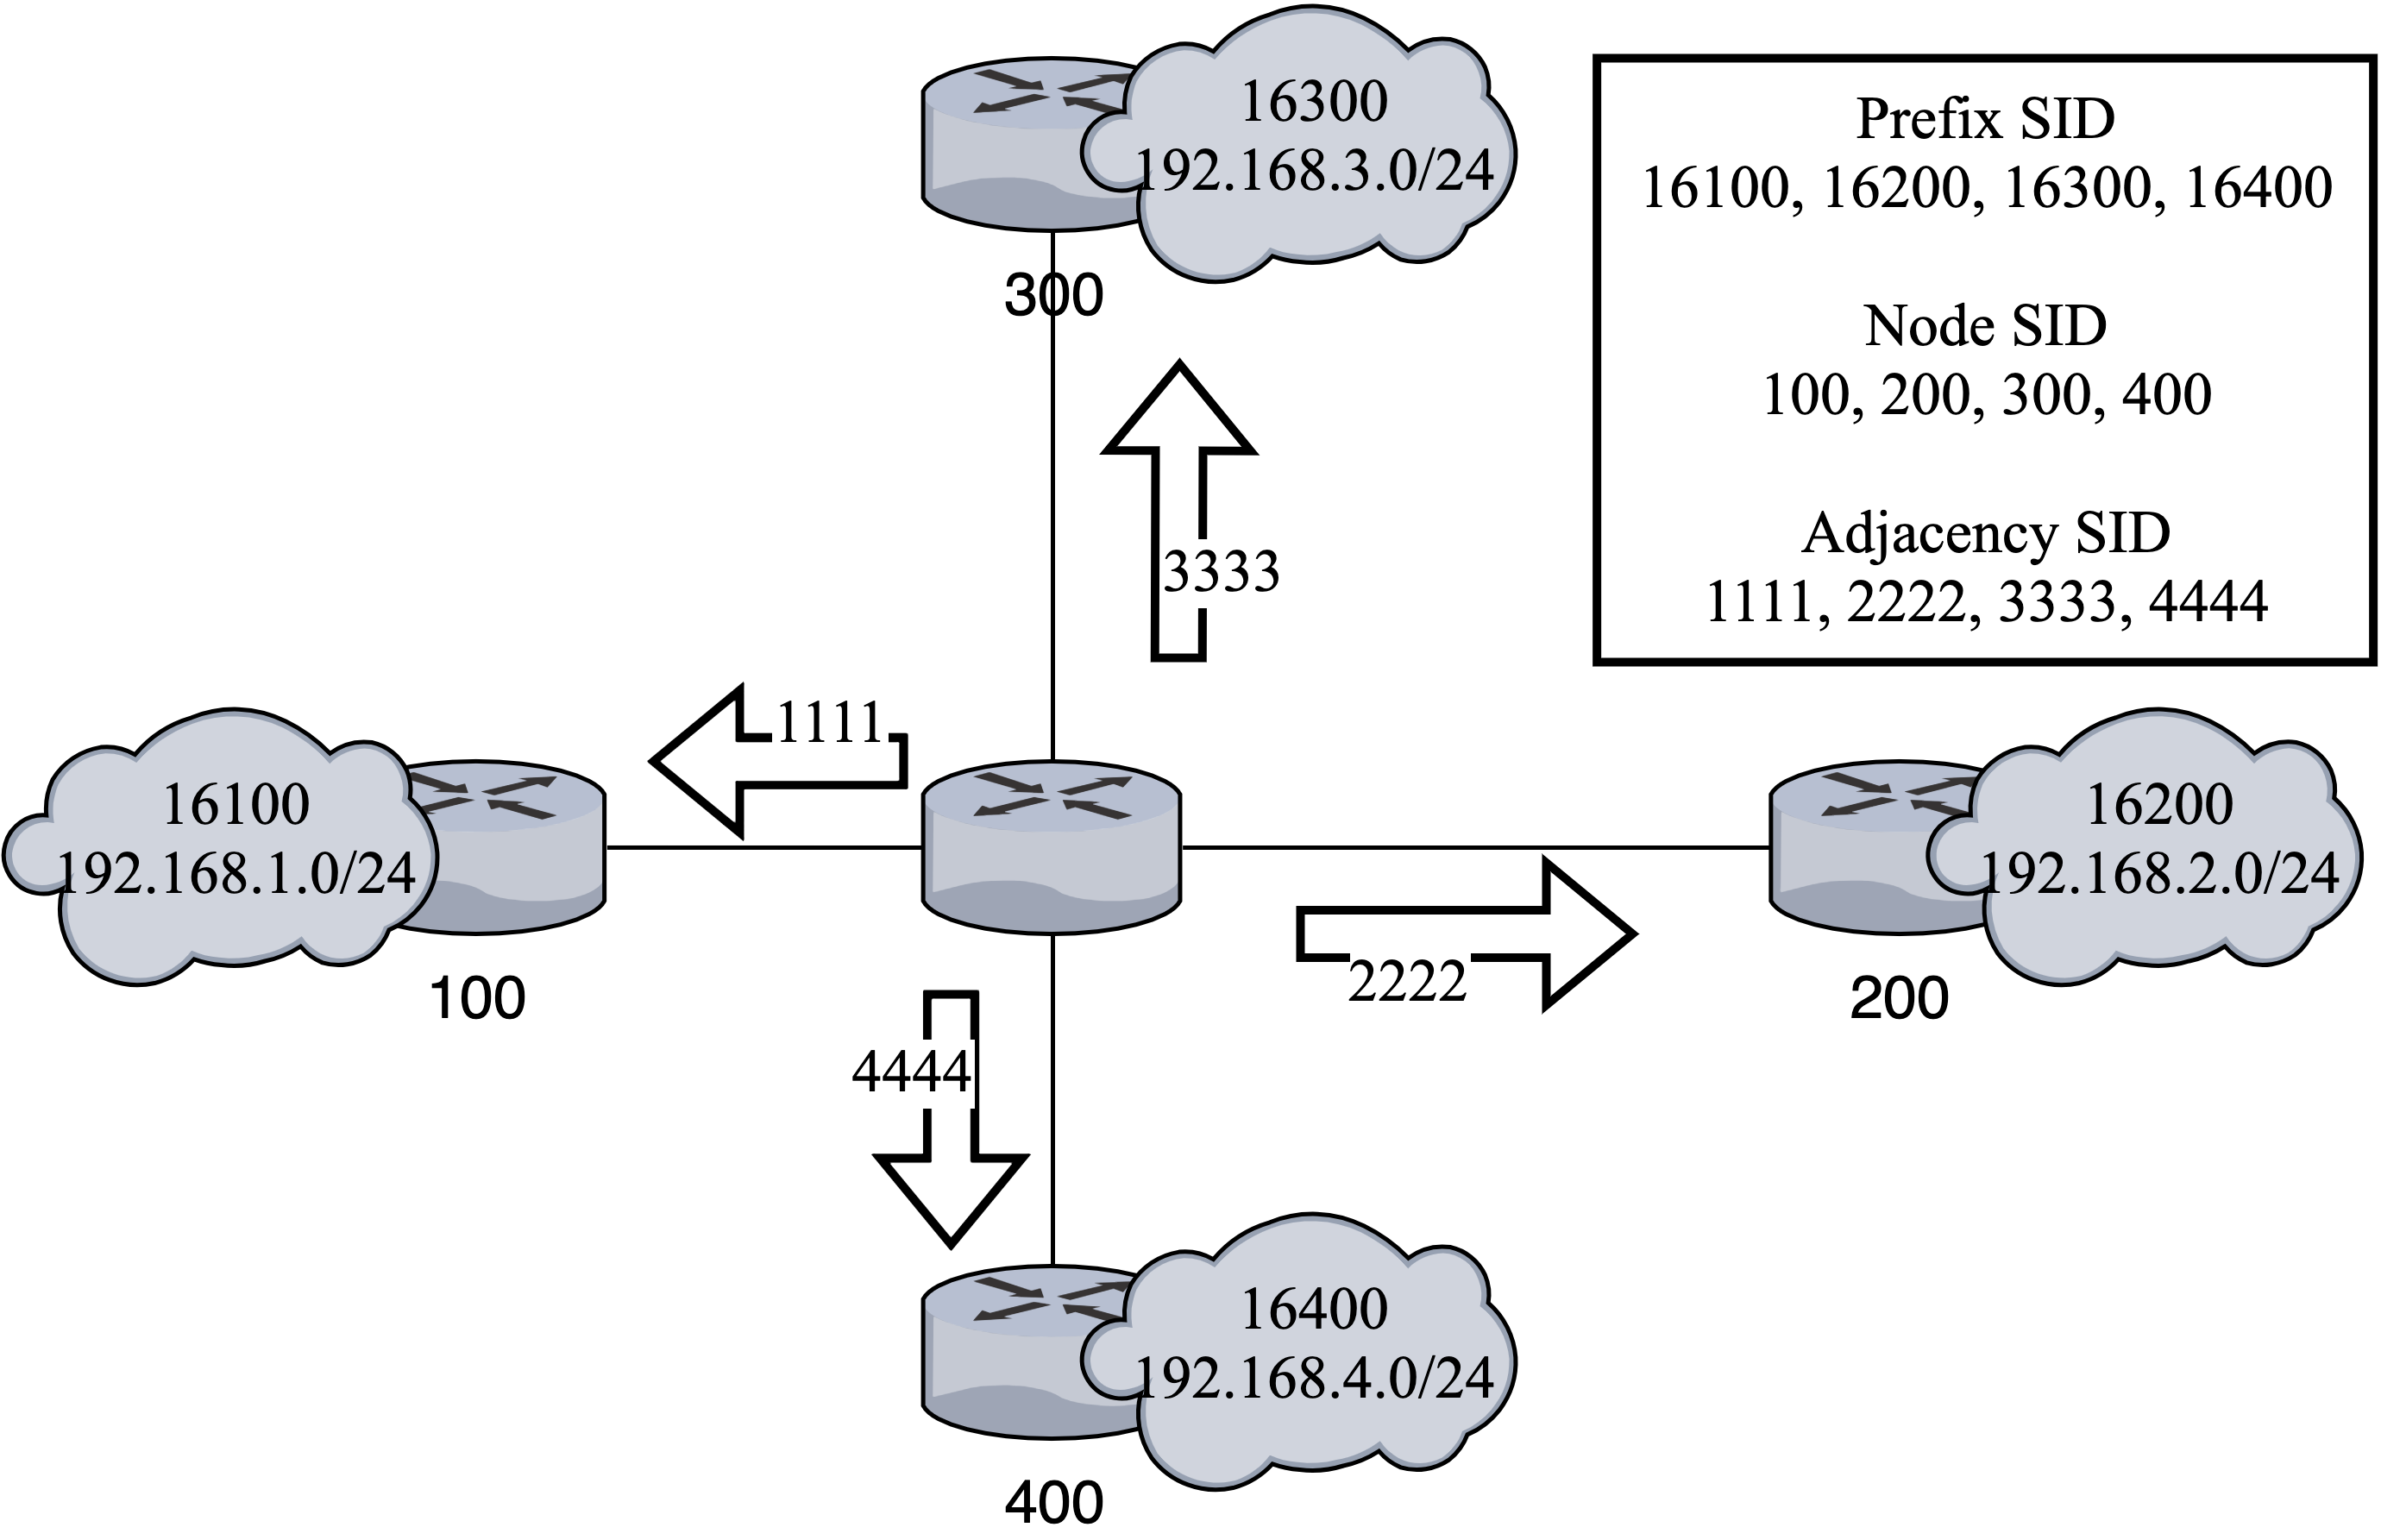
\includegraphics[width=0.9\textwidth]{./figures/ch2-kinds-of-SID.png}}
\caption{段标签的类型及其用途示意图}
\label{fig-ch2-kinds-of-SID}
\end{figure}

段路由节点通常支持以数据平面下操作:基于活动段执行的转发的CONTINUE操作;在数据包的段路由报文头之前添加一个段,并将该段设置为活动段的PUSH操作;以及将下一个段标记为活动段NEXT操作 \cite{SRARK} ,如图2-2所示。

\begin{figure}[htbp]
\setlength{\abovecaptionskip}{15pt plus 3pt minus 2pt}
\centerline{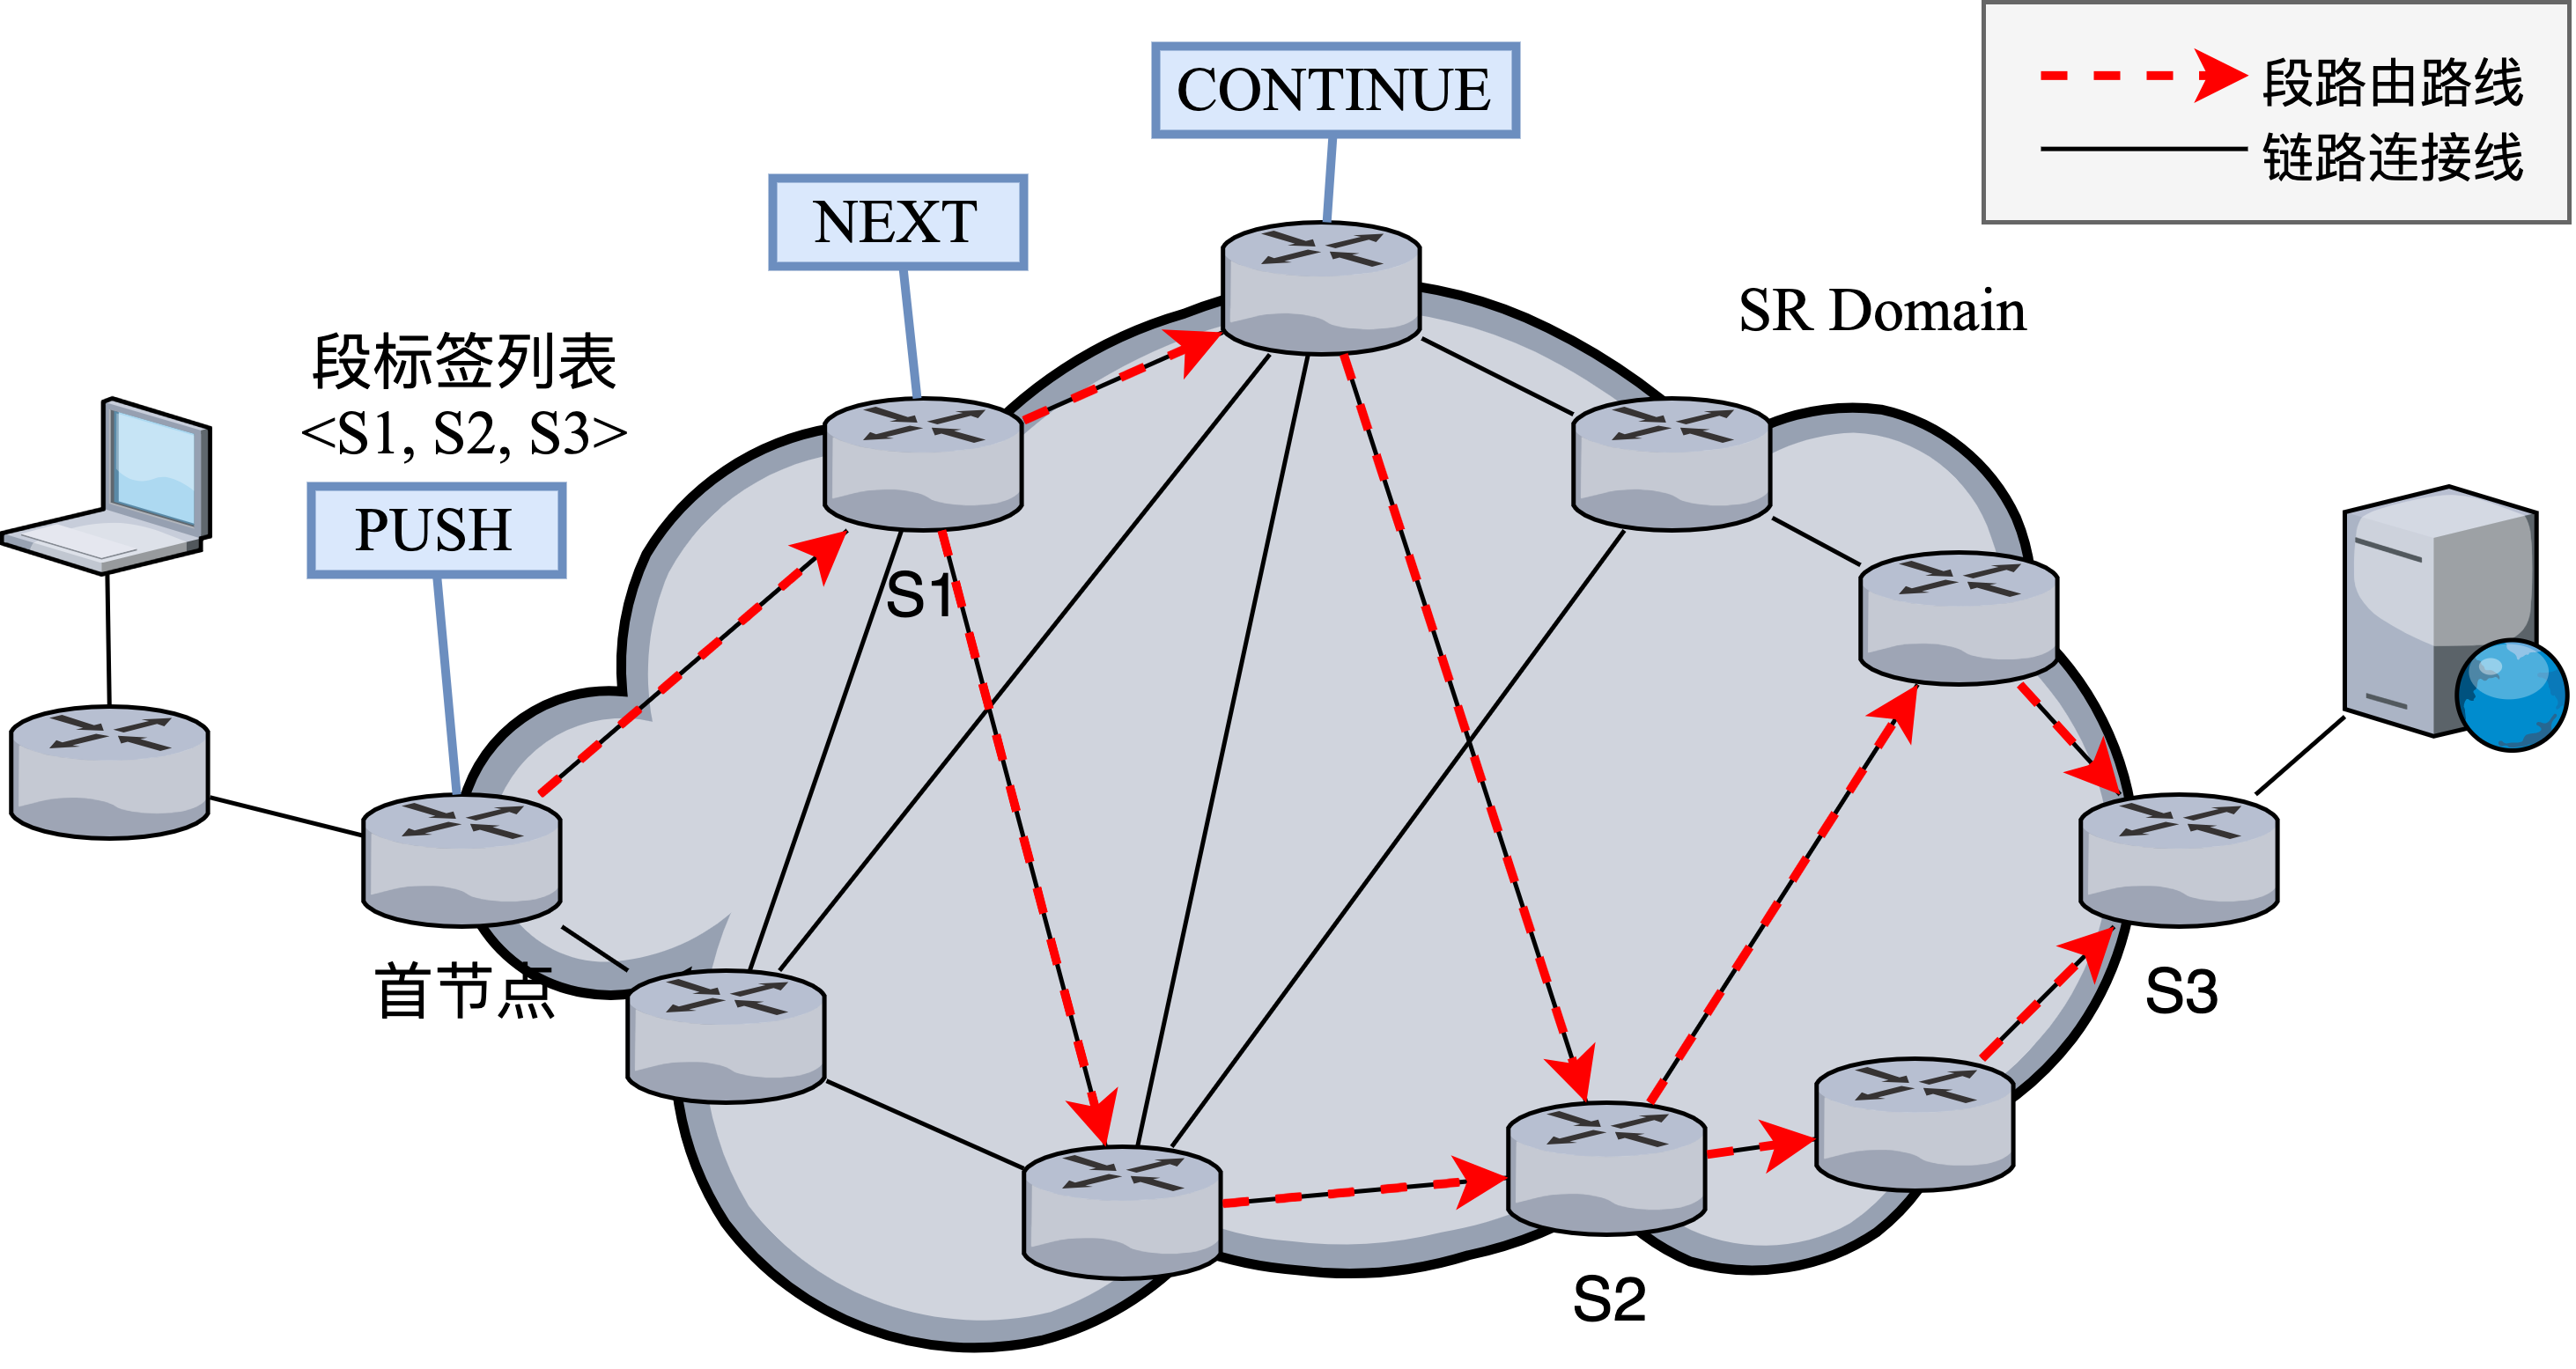
\includegraphics[width=0.9\textwidth]{./figures/ch2-SR-actions.png}}
\caption{段路由节点操作示意图}
\label{fig-ch2-SR-actions}
\end{figure}

如上文所提到,段路由主要有两种数据面类型,基于IPv6的段路由(SRv6)和基于 \gls*{MPLS} 的段路由(SR-MPLS)\cite{SRMPLS}  ,两种数据面功能相似但又有很多不同,功能对比如表2-1所示,SRv6在网络编程上有很大的优势,但是由于其不随路弹出标签的特点和IPv6地址占资源较大的特点,在协议开销、带宽承载效率和 \gls*{MTU} 以及硬件处理效率等资源需求很大,因此现在有一些研究 \cite{GSID} \cite{MICROSID} \cite{USID} 也着眼于压缩段路由报文头,例如uSID \cite{USID} 只包含MPLS的20bit的段标签信息的优化方案。

\begin{table}[]
\resizebox{\linewidth}{!}{
\begin{tabular}{|l|l|l|}
\hline
数据面方案 & SR-MPLS & SRv6 \\ \hline
协议开销 & 4*5=20B & \begin{tabular}[c]{@{}l@{}}16*4\textasciicircum{}2(Segment 列表)+8B(SRH)\\ +40B(IPv6 报头)=112B\end{tabular} \\ \hline
有效负载承载效率 & 440/(20+440)=95.7\% & 440/(112+440)=79.7\% \\ \hline
MTU & 1520B & 1612B \\ \hline
\begin{tabular}[c]{@{}l@{}}对硬件\\ NPU/ASIC 要求\end{tabular} & \begin{tabular}[c]{@{}l@{}}最多只需读出前 20B(标签栈)\\ +20B(IPv4 报头,用于负载均衡)\\ 报头信息即可转发。执行的操作是 \\ SR-MPLS 定义的标准“压入”、\\ “交换”和“弹出”标签操作\end{tabular} & \begin{tabular}[c]{@{}l@{}}需要读出前 112B 报头信息才能\\ 转发执行的操作类型接近 20 种,\\ 包括Underlay、Overlay 和服务\\ 编程等,并且还在不断扩展之中\end{tabular} \\ \hline
\begin{tabular}[c]{@{}l@{}}转发过程是否弹出\\  Segment\end{tabular} & \begin{tabular}[c]{@{}l@{}}弹出。栈顶标签即为活动\\ Segment\end{tabular} & \begin{tabular}[c]{@{}l@{}}不弹出。通过 Segment Left 指针\\ 标识出活动 Segment\end{tabular} \\ \hline
负载均衡实现 & \begin{tabular}[c]{@{}l@{}}一般根据净荷的 IP 5 元组进行哈希;\\ 如果 Segment 数量多,需要使用\\ Entropy 标签\end{tabular} & \begin{tabular}[c]{@{}l@{}}根据外层 IPv6 报头的 Flow Label\\ 字段进行哈希\end{tabular} \\ \hline
\begin{tabular}[c]{@{}l@{}}对网络中间航路点\\ (非头端)的要求\end{tabular} & \begin{tabular}[c]{@{}l@{}}低。由于 SR-MPLS 的开销小,\\ 而且会逐步弹出,因此中间节点\\ 查找的难度不大。主要的挑战\\ 在于在标签栈数量多时,如何\\ 实现有效的负载均衡\end{tabular} & \begin{tabular}[c]{@{}l@{}}高。由于 SRv6 不弹出 Segment,\\ 因此即使是中间航路点,也需要\\ 读取整个 SRv6 报头。\end{tabular} \\ \hline
\end{tabular}}
\caption{SR-MPLS和SRv6区别整理表}
\label{table-SR-MPLS-SRv6}
\end{table}

2. 段路由控制面

段路由的控制平面定义了分段编码信息如何在网络中的设备之间进行通信。在段路由网络中,节点段编码和邻接段编码将通过链路状态内部网关协议进行通告。中间系统到中间系统协议和开放最短路径协议是服务提供商网络中最流行的内部网关协议,它们被扩展为支持分段编码的通告和分配[10],[11]。内部网关协议的扩展将允许任何路由器维护所有节点和邻接段的数据库。此外,通过利用两个内部网关协议的亚秒级收敛特性,可以在任何拓扑更改后快速更新每个路由器上的分段数据库。请注意,使用这些扩展,可以在网络中执行端到端封装,而无需启用和管理其他协议,例如标签分发协议。

段路由控制平面的另一个元素涉及如何指示入口路由器选择数据包应遵循的段路由路径。为此,可以使用以下方法:

\begin{itemize}
\item 分布式 \gls*{CSPF} 计算方法。在这种方法中,入口路由器计算目的地的最短路径,条件是该路径符合某些标准。然后计算对这条路径进行编码的一系列节点和邻接段;
\item 基于软件定义网络控制器的方法。段路由提供了一个可扩展和有弹性的数据平面,同时允许软件定义网络环境通常假设的控制灵活性。这方面导致计划在一些面向软件定义网络的控制器设计中支持段路由。例如, Open Daylight控制器 \cite{ODL} 支持使用 \gls*{PCEP} 控制段路由,如图2-3所示。另外,段路由隧道的静态配置可能用于特定目的,例如测试或故障排除,但由于明显的可扩展性、弹性和管理限制,通常不建议将其用于长期网络操作。
\end{itemize}

\begin{figure}[htbp]
\setlength{\abovecaptionskip}{15pt plus 3pt minus 2pt}
\centerline{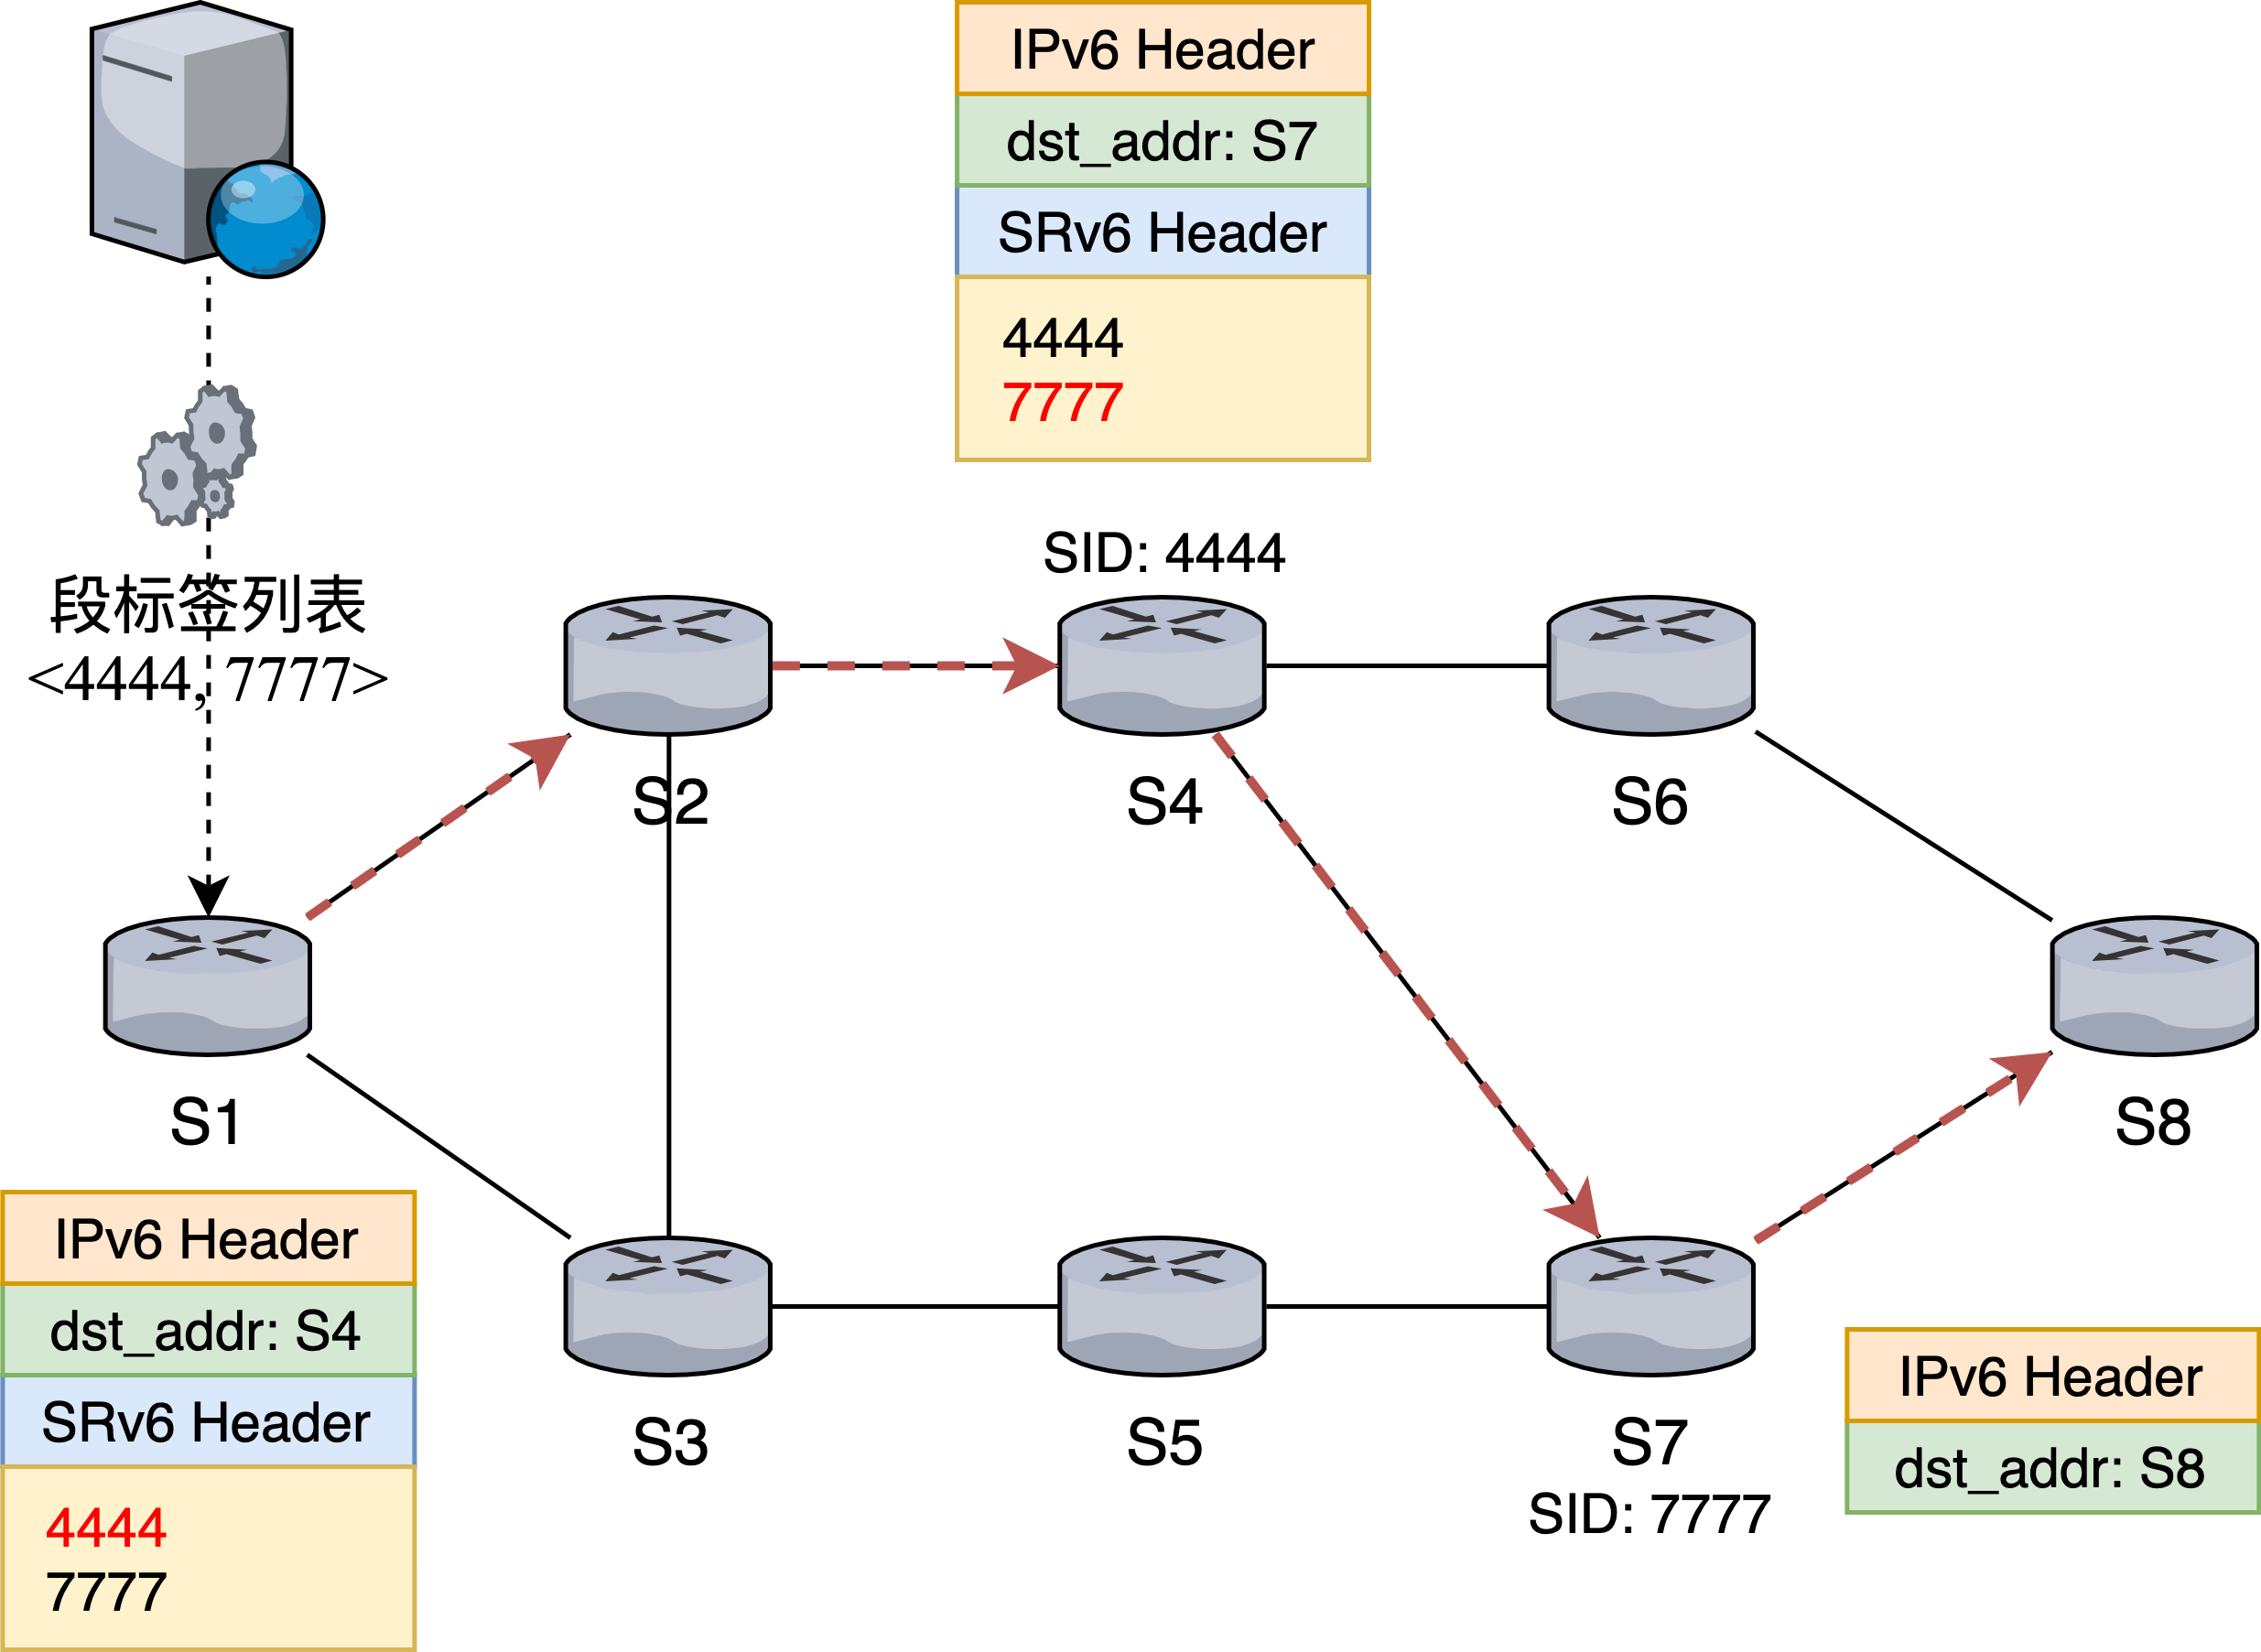
\includegraphics[width=0.9\textwidth]{./figures/ch2-sr-model.png}}
\caption{集中式控制面段路由模型}
\label{fig-ch2-sr-model}
\end{figure}
    
综上所述,段路由控制面可以支持集中式的控制器的标签分发和规则制定,也可以支持分布式的基于域内网关协议和域间网关协议的标签配置,两者的选择可以根据网络的具体情况来制定。

3. 段路由流量工程研究

由于段路由具有对于普通流量不指定路径进行自动负载,对于需要调度的流量计算出显式路径,并下发段路由策略来指导交换机执行的优势。段路由支持网络编码的特点在路由灵活性方面具有格外吸引人的优秀特性,因此段路由被广泛用于流量工程服务保障相关的问题。一些调查显示 \cite{SRSURVEYS} ,有22篇论文利用段路由来提供先进的流量工程解决方案。流量工程的研究工作通常都采用优化问题的经典模型结构:第一必须最小化/最大化目标函数,第二从模型中抽象出一组值得考虑的参数,以及第三考虑特定的网络场景。调查的文献中通常涵盖了三个不同的流量工程目标,即最小化网络能耗、优化拥塞和最小化被拒绝请求的数量。段路由与使用最短路径算法的协议有一个显著不同的地方在于段路由允许的高灵活性的路由路径,这可能会导致数据包在转发中出现复杂而冗长的网络路径。因此,段路由技术在根据特定目标优化段路由航点列表的同时,重要的是要考虑过于复杂的路由解决方案可能对网络性能,如吞吐率产生的影响。除了端到端延迟之外,一些审查的工作还考虑了与段路由相关的开销,包括由于插入段路由报文头的数据包而浪费的带宽,以及要配置段路由转发策略的边缘路由器的数量。最后,还有一些研究着重对网络部署情况进行讨论,所考虑的网络可以是完整的段路由网络,即所有节点都具有段路由能力,也可以是部分节点部署段路由技术的网络,后者中只有一部分节点可以处理段路由报文头,其他节点只能按照网络层协议进行浅层次的转发。由于在数据包中插入段路由报文头而浪费的带宽,以及要在边缘路由器中配置的段路由转向策略的数量。最后,所考虑的网络可以是完整的段路由网络,即所有节点都具有段路由能力,或者是部分部署的段路由,其中只有一部分节点可以处理段路由报文头。

\section{时延研究}

如今,越来越多的应用和平台对低延迟的要求越来越高。然而,在提供低延迟路由服务的广域网中开发新的路由协议非常具有挑战性,并且由于兼容性、可行性、可扩展性和效率方面的障碍,仍然是一个悬而未决的问题。时延相关研究在数据链路层和传输层已经有了很多的研究进展,例如时延敏感网络。由于以太网通信基于尽力而为原则,以太网网络中的数据交换缺乏确定性。到目前为止,以太网中的确定性数据交换只能通过专有解决方案实现,但时间敏感网络旨在改变这种状况。时间敏感网络是一项即将推出的新技术,其重点是通过设计使以太网具有确定性。时间敏感网络是指一组IEEE 802标准,默认情况下使以太网具有确定性。时间敏感网络是一项即将推出的新技术,它位于开放系统互连模型网络架构的第2层。它添加了定义以保证以太网网络中的确定性和吞吐量。以下是构成时间敏感网络的一些 IEEE 标准:增强的同步行为(IEEE 802.1AS)、暂停(抢占)长帧(IEEE 802.1-2018)、计划流量的增强功能(IEEE 802.1Q-2018)、路径控制和带宽预留(IEEE 802.1Q-2018)、无缝冗余(IEEE 802.1CB)、流预留(IEEE 802.1Q-2018)。总而言之时间敏感网络源自业界对音频/视频传输的使用以及对更多设备和同步通信的需求。网络上的设备比以往任何时候都多,共享和分析的信息也更多。因此,以太网必须表现得更好是有道理的。

同样,网络层作为数据中心、运营商提供服务的重要组成部分,提供更可能保障时延的服务也是重要的研究方向,和时间敏感网络这种数据链路层技术不太一样,时间敏感网络可以通过对硬件功率的调整完成无排队的数据链路层网络环境,但是网络层的IP协议已经无法对硬件作出过多干涉,因此需要在IP层独特的技术上作出时延保障优化,而众所周知IP网络层最重要的技术是提供分组交换,分组交换的重要基石就是路由算法。路由算法在很长一段时间一直是基于带宽用最短路径算法进行路由分配的,考虑将时延信息加入各种路由算法是值得考虑的地方。

\section{带内遥测}

随着软件定义网络和可编程数据平面技术的发展,带内网络遥测应运而生。带内网络遥测技术通过业务报文逐跳收集网络状态信息,实现网络服务的端到端可视化。带内网络遥测利用数据平面直接驱动网络测量过程,颠覆了传统网络测量将网络交换设备视为中间黑匣子的研究思路。带内网络遥测技术具有编程灵活、实时性强、噪声小、路径级网络状态感知等优点,已成为网络遥测技术的新兴代表,受到学术界和工业界的广泛关注。带内遥测可以用于测量交换机提供的各种信息,例如带宽、时延、排队队列等。

在带内遥测采集单向时延的研究 \cite{INTSURVEY} 上,Kim等结合带内遥测路径定位信息和交换机排队时延信息,实现基于 \gls*{HTTP} 应用的瞬时时延测量;Mizrahi等使用少量的比特来标记业务数据包,遥测服务器计算网络的逐跳延迟;Riesenberg等基于Marvell的Prestera芯片和 \gls*{P4} 编程语言,采用双标记测量时延使得时延误差小于100纳秒,丢包率测量误差几乎为零;IntMon等基于 \gls*{ONOS} 控制器和编程独立于协议的数据包处理器的 \gls*{BMv2} 软件交换机的对使用 \gls*{UDP} 封装带内遥测进行了尝试并实验验证其有效性。而在在带内遥测采集双向时延的研究上,Pingmesh通过主动 \gls*{Ping} 操作检测数据中心网络延迟变化实现双向带内遥测数据的采集。EverFlow则发送探测以测试和确认潜在的网络故障,已经经常用于数据中心网络的数据包级网络遥测系统。

因此可见对时延数据进行带内遥测的技术已经相当成熟,时延也逐步取代带宽成为网络中更值得关注的网络服务性能类型。这在拥塞控制技术中已经得到了相当多的应用。例如谷歌2020年获得的Sigcomm最佳论文的Swift模型 \cite{SWIFT} 中就使用的主要拥塞信号就是时延,因为它满足了工程师对拥塞感知的所有要求。谷歌在Swift这篇论文中指出,网络往返时延可以使用现代硬件精确测量,并且它提供了多位拥塞信号,即它不仅对拥塞的状态进行编码,而且对拥塞的程度进行编码。Swift进一步分解了端到端往返时延,以将架构与主机问题分开;通过结合网卡硬件中的时间戳和基于轮询的传输(如Pony Express),它使延迟测量更加精确。Swift使用多个网卡和主机时间戳来分离延迟的组成部分,并进而将网卡收方向数据包延迟和处理时间相加以获得全程排队时延,并通过 \gls*{ACK} 数据包上的报文头将此延迟反映给发送方。

因此使用带内遥测技术作为时延采集的方式是可行的,本研究在后文中不对带内遥测做过多分析,只是使用这一项技术作为时延信息采集的渠道。在实验验证阶段也是采用符合逻辑的遥测方式获取时延。


\chapter{基于时延的集中式段路由航点生成算法}

\section{引言}

本章将以集中式软件定义网络控制器的视角对基于时延的段路由航点生成算法进行问题建模分析,核心算法阐释,并通过仿真实验验证算法在尽力保障时延的有效性。

\section{问题模型}

段路由网络中具有非段路由节点和段路由节点,控制器通过带外控制链路和段路由节点通信,控制器需要分配、通告段路由标签,并按照到达数据包的时延需求计算段标签列表,如图3-1所示。将网络中的交换机抽象成节点,链路抽象成双向有向边,构成有向图$G(V, E)$。假设任何一个节点$v$都有可能有流量到来,$f(s, d)$ 表示源节点为$s$,目的节点为$d$的待服务流量,在真实IP网络中,一般用源地址、目的地址、源端口、目的端口、协议组成的五元组来标识一个流量,但是在问题建模中,不需要考虑传输层的端口号和具体协议号,因此只需要用源地址、目的地址 $f(s, d)$ 来标识一条流量。

\begin{figure}[htbp]
\setlength{\abovecaptionskip}{15pt plus 3pt minus 2pt}
\centerline{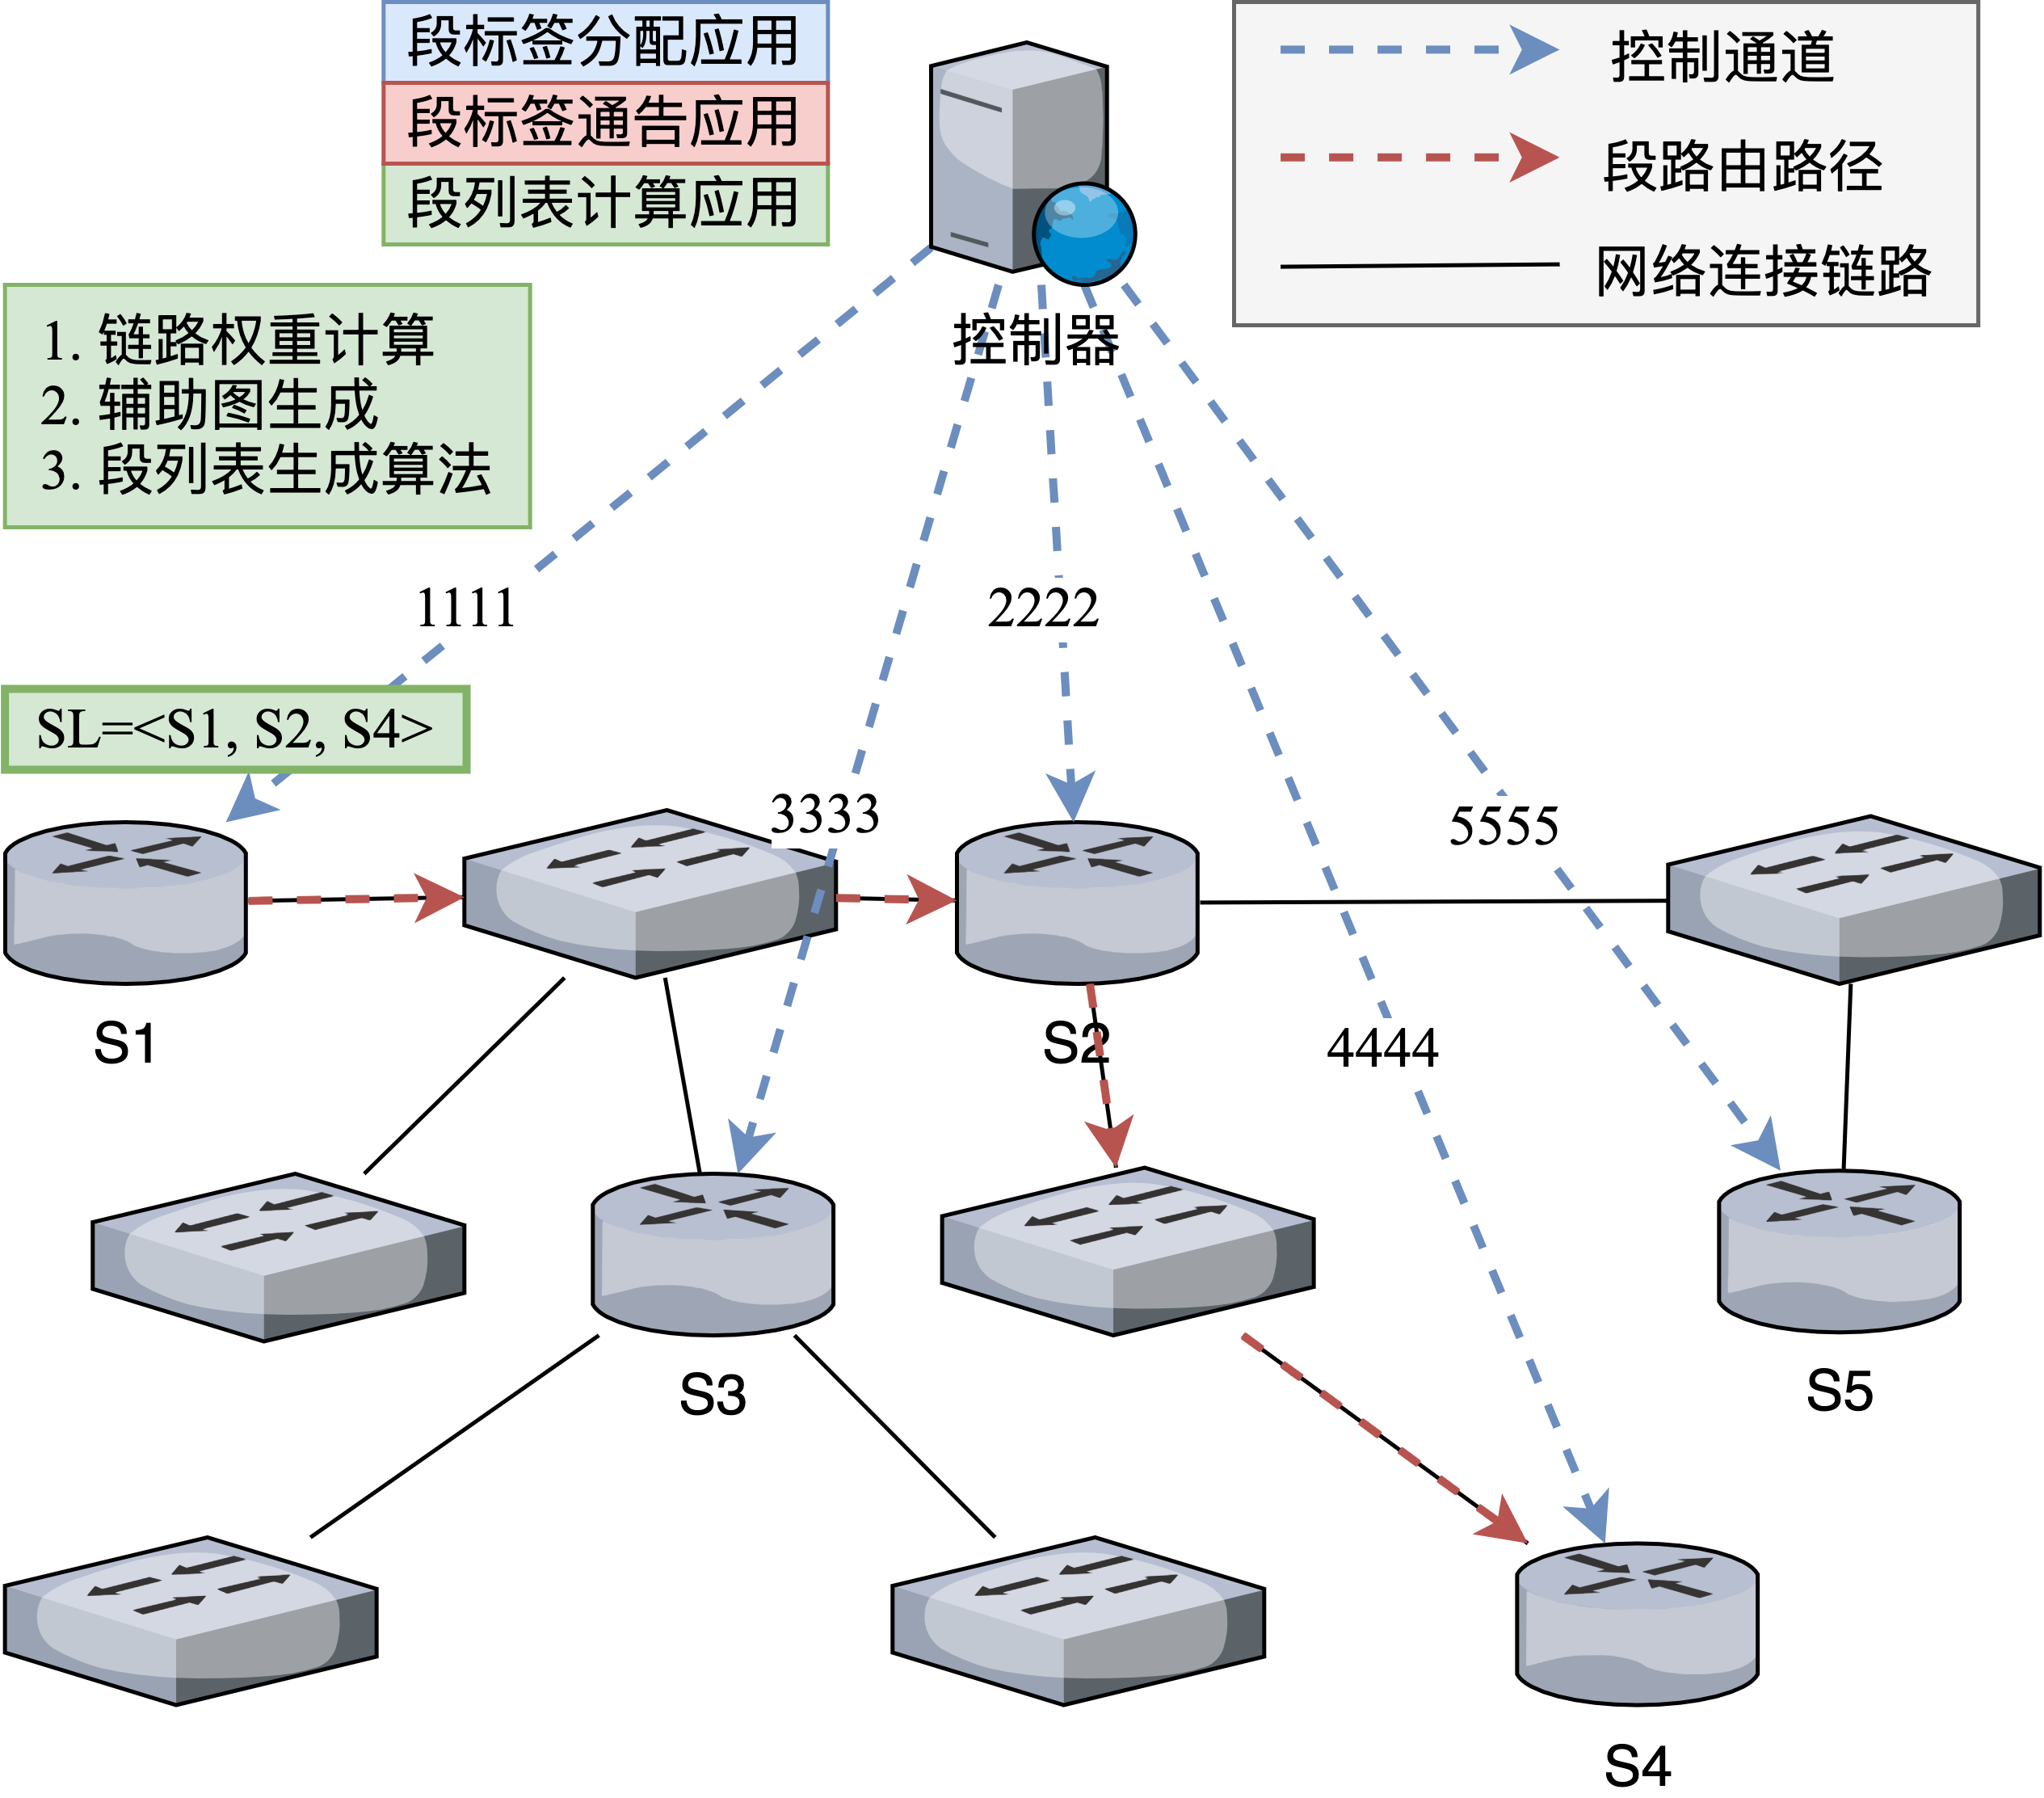
\includegraphics[width=0.8\textwidth]{./figures/ch3-problem-model.png}}
\caption{集中式段路由控制面问题模型}
\label{fig-ch3-problem-model}
\end{figure}

因此将问题建模为:已知有向图$G(V, E)$,流量$f(s, d)$,计算出一组段标签,使得流量通过这组段标签的时延较短。

\section{基于时延的段路由航点生成算法}

\subsection{算法概述}

段路由航点生成算法本质上是一个最优路径选择问题。在弱约束的情况下,最优路径选择是一个完全非确定多项式(Complete Nondeterministic Polynomial, NP-complete)问题。在[XX]中,研究了基于软件定义网络的广域网中的段路由流量工程,并证明一般的段路由标签列表选择问题是一个非确定多项式难题(Hard Nondeterministic Polynomial, NP-hard),非确定多项式难题代表如果解决一个问题的算法可以转化为解决任何非确定多项式问题的算法,那么这个问题就是非确定多项式难题。即非确定多项式难题意味着“至少和任何非确定多项式一样难”。如果段路由只允许每条路径有固定数量的$M$个中间点,那么具有最短路径的流量工程是弱多项式可计算的。覆盖面最广的方法是将所有节点视为候选中间点,将网络拓扑中的全部节点标记为V,候选节点标记为$C$,则有$C = V$。然而这会导致解决一个流量工程资源分配问题的程序的成本会非常高昂。另一种方法是只考虑少量的中间节点,例如$C=k|V|$,这里$k$是一个比例系数,虽然只是使用了一部分全部网络拓扑的节点进行计算,这仍然会为流量工程的需求输出出性能良好的方案。这里提到的中心度概念只是关注网络拓扑图结构的结构度量,即各个节点之间的连接关系。在研究[XX]中表明当中间点的数量固定而不是输入的一部分时,流量工程路径问题可以在弱多项式时间内解决。但是如果有固定的参数来约束,该问题可以在多项式时间内解决。因此段路由标签列表的长度被用来限制研究中的段列表生成算法。一般来说,深度为2的段列表可以有更好的交通分流效果。在[24]中,作者分析了现实世界的交通,并扩展了2-段路由公式,以最小化非最短路径隧道的数量。他们还评估了3-段路由和4-段路由的流量工程能力,表明它们非常耗时。因此在本研究中,段路由标签列表的长度被限制为2或3,段列表长度的影响在实验中得到了验证。最后贝尔曼-福特算法将被用于计算段路由标签列表基于上述问题的建模和限制条件。

总结上述内容,本章将讨论的主体有两个部分,第一个是如何设计出考虑时延状态的链路权重计算公式,第二个是如何优化原本为非确定多项式难题的段路由航点生成算法。问题一将在3.3.2进行讨论,问题二的优化方法则是分为两个部分,第一个是如何选择少量的节点基于具有多项式复杂度的替代中心度度量的实用中间点选择,解决这个问题的方法是辅助图生成,将在3.3.3进行讨论,第二个问题则是如何限制最优路径选择问题中的迭代次数问题,使其从非确定多项式难题转变为多项式时间解决问题,这个问题的解决方案是限制段标签列表的深度,将在3.3.4进行讨论。

\begin{figure}[htbp]
\setlength{\abovecaptionskip}{15pt plus 3pt minus 2pt}
\centerline{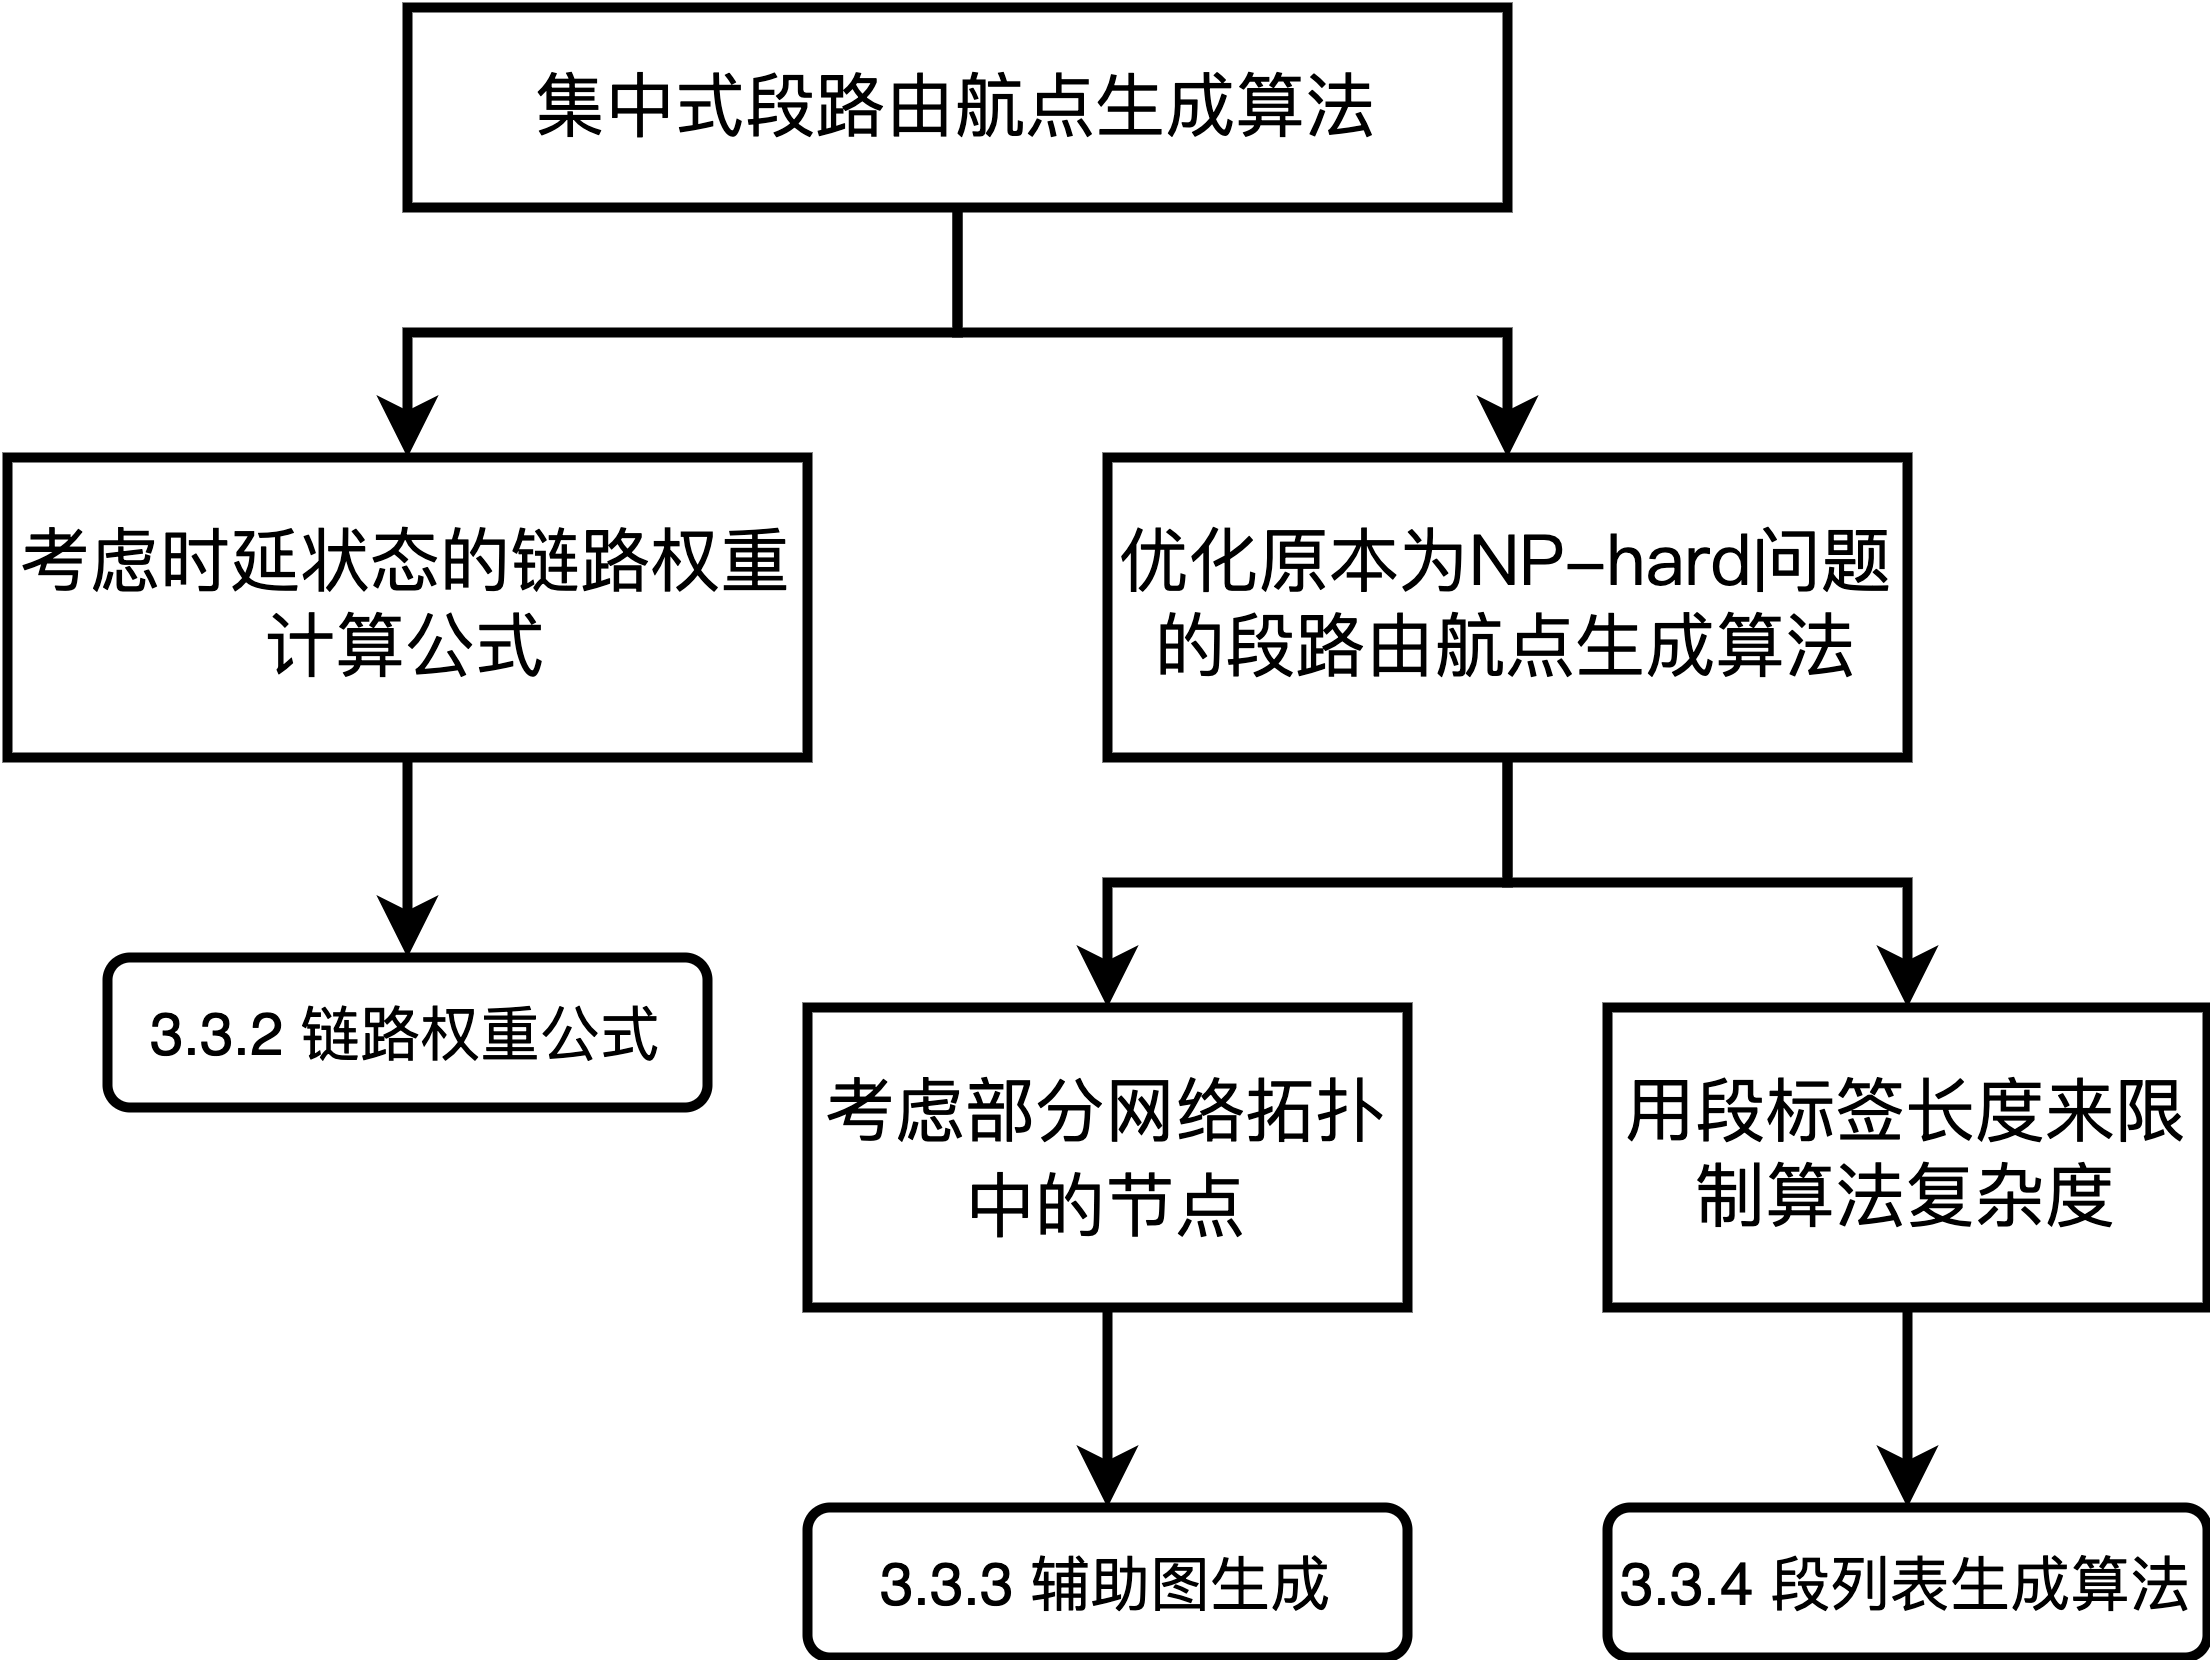
\includegraphics[width=0.8\textwidth]{./figures/ch3-ark.png}}
\caption{集中式段路由航点列表生成算法思路索引结构图}
\label{fig-ch3-ark}
\end{figure}

对于基于时延段路由的航点生成算法来说,主要步骤有三步:第一步是静态场景下计算链路权重,第二步是在原有拓扑上生成拓扑数目为了将时延更好地结合到节点选择的算法中,本文没有直接将通常用带宽进行估算和权重衡量的方案直接替换成采集到的时延参数,而是将时延信息和带宽进行综合分析并构建出权重公式。基于构建出的权重公式在较为静态的网络环境下计算各个链路的权重。并且在基于静态情况下对网络节点的权重进行计算,选择相对较为核心的节点构造辅助图,辅助图将是节点选择算法中选择节点对象的集合,这是因为选择中心度更高的节点在调流上会达到更好的效果。试想如果一个节点被各种情况下经过的概率更高,那么选择其他节点也都会有更大的概率达到这个节点,辅助图节点集合的确定就是为了缩小节点选择范围使得后期遍历的算法复杂度降低。最后我们通过贝尔曼-福特算法得出段路由需要的航点列表,选择贝尔曼-福特算法而非迪杰斯特拉等最短路径算法的原因主要是考虑到负权重路径的存在。

本节剩下的章节将对以上提到的三个算法点进行详细的解释。

\subsection{链路权重公式}

通常来说,网络流量图以及流量工程矩阵都是以带宽为度量数据的,因此在有向图$G(V, E)$中如何考虑时延制定有向边的的权重是第一个需要明确的问题。在本节中,本文考虑到拓扑因素、延迟效应和带宽限制,从这三个角度构建了一个通用衡量的链路权重的表达式。

1. 链路中心度

本文用链路中心度量化拓扑因素。已知$(s,d)$表示网络中可能产生通信需求的源节点和目的节点,则令$S_{sd}^k$表示这一对源节点和目的节点$(s,d)$之间前k条最短路线的集合。令$e$表示网络中的每条有向链路,领$f_{sd}^k(e)$表示链路$e$在源节点$s$到目的节点$d$的前$k$条最短路线路径中出现的频率。

基于上述定义,$f_{sd}^k(e)/k$可以被视为$(s,d)$之间前$k$条最短路径中链路$e$的出现率。因此,本文计算流量矩阵中可能产生通信的每一对节点之间的前k条最短路径,并将$e$出现的频率相加。这个频率的总和用于确定网络中链接$e$的中心度,它的含义是在链路$e$在各种网络层路由算法中被选中的可能性,因此链路$e$的链路中心度$c(e)$使用各个节点对的$f_{sd}^k(e)/k$的累积加和来计算。相对于流量变化的频率,网络拓扑从结构上来看基本是处于静态的。因此,本算法需要在静态阶段针对网络中所有可能的通信路径,用如迪杰斯特拉等最短路径算法计算出$(s,d)$的前$k$条最短路径,这个时间复杂度是$|V|\cdot O({|E|}^2)$。但是链路中心度并不是需要一直计算的,只有在网络拓扑出现变化的时候才需要更新,可以说这个参数是事件驱动的,并不会长时间占用控制器的计算资源。
$$c\left(e\right)=\sum_{\forall(s,\ d)\in T M}{f_{sd}^k\left(e\right)}/k$$

设计链接中心度$c(e)$的意图是表征等价多路径路由选择特定链接$e$的可能性,等价多路径路由常用于IP网络中作负载平衡,只要路径跳数相等即视为等价,就可以流量在这些路径上负载均衡。因此$c(e)$越大,任何两点产生通信时,数据流量通过$e$的概率也就越大。

2. 链路到达率

从本质上讲,交换机端口的排队延迟是由于数据包的到达但没有得到及时处理而造成的。根据排队理论中对任何到达和服务分布都成立的利特尔法则(Little's law):$W_q=L_q/\lambda$,可以得到以下推断。

在利特尔法则中$W_q$是排队问题的平均等待时间,$L_q$是平均队列长度,$\lambda$是到达率。到达率衡量的是顾客进入队列的速度。经过转换利特尔法则,就可以得到$\lambda$的计算公式。$\lambda=W_q/L_q$。此外,当到达率小于服务率时,排队系统可以得到平衡。

交换机模型中的平均队列长度$L_q$可以用单位时间内通过定向链路$e$的数据包数量来衡量,定向链路实际上就是交换机端口发送的 \gls*{PPS} ,用$p(e)$表示。平均等待时间$W_q$可以用交换机中消息元数据的时间戳来计算。例如,在 \gls*{PISA} 中,$standard_metadata.ingress_global_timestamp$在入口管道开始解析消息并将其添加到消息的原始头中之前使用。为了记录消息到达时间戳的元数据,$standard_metadata.egress_global_timestamp$是在出口管道开始解析消息之前添加在消息的原始头之前的元数据,用来记录消息通过流量管理器到达出口时的时间戳。由于排队的数据包几乎都发生在流量管理器中,这两个元数据的差异可以用来衡量数据包的排队延迟。在交换机中进行统计平均后,可以收集并计算出$W_q$,记录为$d(e)$。因此,交换机中的链路到达率$\lambda(e)$可以用以下公式计算。
$$\lambda(e)\ =\ p(e)/d(e)$$

链路到达率$\lambda(e)$背后的含义是表示未来短时间内是否有大量数据包会到达某条链路$e$上。由于网络中的预测信息是根据历史数据推断出来的,$\lambda(e)$越大,未来需要在链路$e$上服务的到达数据包就越多,排队的可能性也就越大。

3. 链路拥塞度

带宽是计算链路权重时必须考虑的一个问题。带宽和延迟不成比例的一个重要原因是,交换机中的队列只是数据包的头,而不是整个数据包。整个数据包的大小与数据包头的大小无关,这意味着一条链路可能被阻断。小数据包填满了缓冲区,但实际带宽并不反映高负荷。同样,一条链路可能被大数据包填满,缓冲区没有排队或延迟,但链路带宽可能真的有瓶颈。因此,有必要考虑链路e的当前负载是否会影响未来的路由性能。

让$f(e)$表示链路$e$的已用带宽,让$b(e)$表示链路$e$的总带宽,让$r(e)$表示链路$e$的剩余带宽,即,$r(e)=b(e)-f(e)$。

基于上述定义,构建的链路负载率$s(e)$表示链路$e$使用带宽的比例,计算公式如下。
$$s(e)\ =\ f(e)/r(e)$$

链接拥堵指数$s(e)$的定义是一个增加的凸函数。也就是说,$s(e)$越大的链路意味着流量很可能立即爆满,需要避开。

4. 链路权重

为了结合上述三个参数来计算与延迟有关的定向链路的权重,首先我们应该考虑这些参数的特点。
$c(e)$与拓扑状态和$k$的值有关。当$k=1$时,数值范围可以达到$(0,\ count(V_{Host})/2),count(V_{Host})$是网络中可能发起消息的主机节点数量;当$k>1$时,数值范围的上限应该小于$count(V_{Host})/2$。这意味着$c(e)$是一个幅度不太大的参数,它比$\lambda(e)$和$s(e)$的值更固定。

$\lambda(e)$是排队到达率,它与到达交换机的数据包大小有关。根据对数据中心网络情况的观察,$\lambda(e)$的大小在$({10}^5,{10}^8)$之间。为了反映排队到达的计算效果,该值需要接近$s(e)$,所以取$\lambda(e)$的对数,使其接近$s(e)$和$c(e)$。

$s(e)$是一个递增的凸函数,其数值范围为$\left(0,\infty\right)$。当$f(e)$极小时,$s(e)$接近0,$\lambda(e)$会比以前小一点。所以要平衡$s(e)$和$\lambda(e)$的变化。$\lambda(e)$取$10$的对数,得到$\left(5,\ 8\right)$的值,为了增加其影响力,用它作为$s(e)$的指数来参与计算。最后,考虑影响范围,将$c(e)$的权重考虑在内,最后得到有延时的有向链接$w(e)$的权重。

值得一提的是,在链路权重的设计过程中,本文考虑了两种情况。

第一种是当链路完全不拥塞的时候,着重考虑链路中心度,而当链路产生拥塞的时候,考虑链路拥塞度和链路到达率,这种设计方案,需要一个额外的参数来调和这几个参数相加时的比例,例如如下公式:
$$w(e)=\theta \cdot s(e)ln(λ(e)) +(1- \theta )/c(e) \ \  0 \le \theta \le 1$$

第二种利用链路拥塞度的凸函数激增特性,当链路不拥塞的时候,着重考虑链路中心度,而当链路产生拥塞的时候考虑链路到达率,在这其中用链路拥塞度来作为调和比重的参数,由于该参数需要用归一化的方式调和,因此将$s(e)/100$和$1-s(e)/100$作为调和$c(e)$和$\lambda(e)$的系数,如下公式所示:
$$w(e) = c(e) \cdot (e)/100 + \lambda(e) \cdot (1-s(e)/100)$$

下文将对这两种构造方法进行比较得出最终使用的链路权重公式。

当考虑第一种算法时,目的是当链路完全不拥塞的时候,着重考虑链路中心度,而当链路产生拥塞的时候,考虑链路拥塞度和链路到达率。所以将几个不重要的参数设置为常量,其中$e$是一个有向链接,$\theta$是调整链接属性和链接状态的系数。$\theta$是一个保留参数,在后面对此公式进行分析的实验计算中都取为$0.5$。如何为$\theta$取一个更合适的值,需要根据具体的网络进行调整,因为它对平衡链接属性和链接状态很有用。这个公式建议使用临界度较高的链路和具有更多可用带宽和较低链路到达率的链路。因此假定到达率$\lambda\left(e\right)$为$0.5$,$\theta$为$0.5$。对于一个给定的链路$c\left(e\right)$是一个常数,所以随着链路流量的逐渐增加,链路权重的增加趋势如图3-3所示。

\begin{figure}[htbp]
\setlength{\abovecaptionskip}{15pt plus 3pt minus 2pt}
\centerline{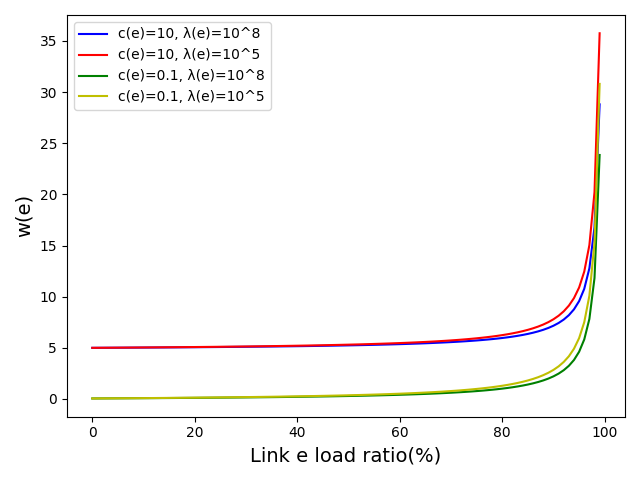
\includegraphics[width=0.8\textwidth]{./figures/ch3-link-weight-function-1.png}}
\caption{第一种链路权重算法下链路权重随链路负载增长变化示意图}
\label{fig-ch3-link-weight-function-1}
\end{figure}

当网络负载较轻时,链路可用带宽和链路到达率都很低,权重函数倾向于参考链路临界值$c\left(e\right)$;当网络负载较重时,链路可用带宽和链路到达率较高,链路权重函数会急剧增加,因此权重函数会倾向于参考链路拥塞指数$s\left(e\right)$和链路到达率$\lambda\left(e\right)$。当网络资源利用饱和时,通过链路拥塞指数$s\left(e\right)$和链路到达率$\lambda\left(e\right)$来确定链路权重是合理的,而不是在拓扑属性下确定链路临界度。

当考虑第二种算法时,目的是当链路几乎不拥塞的时候,着重考虑链路中心度,而当链路产生拥塞的时候,重点考虑链路到达率。这样做是考虑到当链路几乎不拥塞的时候,具有更高链路中心度的链路是可以提供更高联通度的链路,本身就更容易在IP层的哈希中被选中。而当链路产生拥塞的时候,该算法希望能选出那些未来数据包到达率更低的链路,避免竞争。链路权重的增加趋势如图3-4所示。选择链路中心度分别为$0.5$、$0.01$的链路,假设数据包到达率不变分别为$0.5$和$0.01$,将它们两两组合,则可以画出在这4种情况下,使用公式二的链路链路权重随链路负载增加的情况。

\begin{figure}[htbp]
\setlength{\abovecaptionskip}{15pt plus 3pt minus 2pt}
\centerline{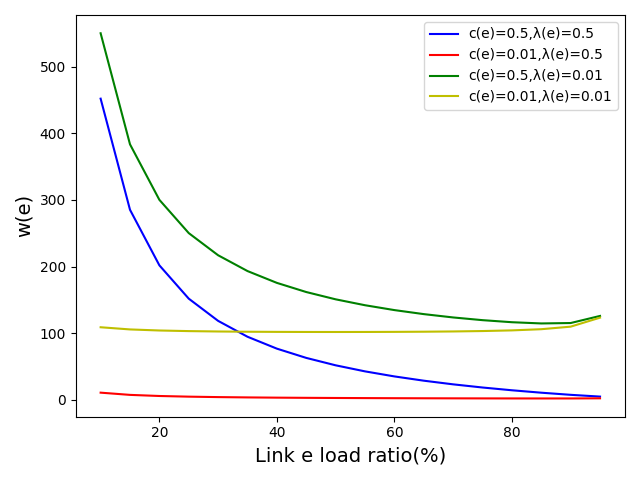
\includegraphics[width=0.8\textwidth]{./figures/ch3-link-weight-function-2.png}}
\caption{第二种链路权重算法下链路权重随链路负载增长变化示意图}
\label{fig-ch3-link-weight-function-2}
\end{figure}

只观察$c(e)=0.5,\ \lambda(e)=0.5$(蓝色折线),可以看出控制链路到达率不变,当网络负载较轻时,链路可用带宽较高,$c(e)=0.5$的链路具有较高的链路权重;当网络负载较重时,链路可用带宽低,链路拥塞度高,造成链路权重下降。

将$c(e)=0.5,\lambda(e)=0.5$(蓝色折线)和$c\left(e\right)=0.01,\lambda\left(e\right)=0.5$(红色折线)对比,控制链路到达率不变时,链路中心度较高的链路一直有较高的权重,而链路中心度较低的链路直到链路带宽基本占用满才和高链路中心度链路具有相同的链路权重。

将$c(e)=0.5,\lambda(e)=0.5$(蓝色折线)和$c\left(e\right)=0.01,\lambda\left(e\right)=0.01$(黄色折线)对比,当网络负载较轻时,权重函数倾向于选择链路中心度$c\left(e\right)$更高的链路,而当网络负载较重时,权重函数倾向于选择链路到达率$\lambda\left(e\right)$更低的链路。即当网络资源利用饱和时,链路拥塞指数$s\left(e\right)$已经很高了,此时通过链路到达率$\lambda\left(e\right)$来确定链路权重而不是用拓扑属性的链路中心度是合理的。

除此以外,方案一的权重函数,在链路中有中心度较高但到达率低的链路又可能不如链路中有中心度低但到达率高的链路权重,这也是不合理的地方,因此经过上问的分析,本算法使用方案二的链路权重函数作为考虑时延情况的链路权重函数。

在评估了链路权重$w\left(e\right)$后,在生成辅助图的边集过程中,权重$w\left(e\right)$小于$\beta$的链路将被删除。所以算法将设置一个阈值,表示为$\beta$,并在生成辅助图时设置$\beta=20$来限制一个链路权重的大小不能过小。

\subsection{辅助图生成}

由于段路由的节点集是整个节点集的一个子集,所以可以不把所有的链接和节点提到计算范畴,而是选择一些节点重建拓扑图,节点的选择主要考虑的是节点中心度,按原有拓扑节点总数的幂次比例的子集作为辅助图节点,进而通过链路属性的筛选来生成一个辅助图以降低拓扑复杂性和计算段标签列表生成的时间复杂度。

1. 节点中心度

本段将讨论基于具有多项式复杂度的替代中心度度量的实用中间点选择。值得注意的是,这些中心度是关于拓扑图本身结构的结构度量量,即主要通过各个节点之间的连接关系来评判中心度。因此这些节点中心度的计算方式一般没有考虑网络中存在流量的情况,也不会考虑网络流量守恒和容量约束等问题。这里将讨论三种节点中心度度量方式,分别是最短路径中心度、组最短路径中心度、度数中心度,评判三种常见中心度的侧重最终得出本文使用的节点中心度计算公式。

最短路径介数中心度根据随机选择的源-目的地址对,通过该节点v的最短路径的数量就是可以表征节点v的中心度的度量量。具体而言,假设在有向图$G=\left(V,E\right)$中,节点$v \in V$的最短路径介数中心度定义为:
$$\delta\left(v\right)=\sum_{s,t\in V|s\neq v\neq t}\frac{\sigma_{st}\left(v\right)}{\sigma_{st}}$$

其中$\sigma_{st}\left(v\right)$是从$s$到$t$通过$v$的最短路径数,$\sigma_{st}$是从$s$到$t$的最短路径总数。计算图中所有顶点的最短路径中心度需要$\Theta({|V|}^3)$时间和$\Theta({|V|}^2)$空间。这可以通过增加弗洛伊德算法解决所有对最短路径问题的路径计数来实现。而在未加权和加权网络上改进这些时间复杂度界限则可以通过中介中心性布兰德斯算法(Brandes算法),布兰德斯算法算法是计算中介中心性近似分数的最著名算法,它不计算每对节点之间的最短路径,而是只考虑所有节点的一个子集。布兰德斯算法可以通过仅使用$\Theta(|V|+|E|)$空间并在$\Theta(|V|+|E|)$和$\Theta(|V|\bullet|E|+{|V|}^2log|V|)$中运行来分别改进未加权和加权网络上计算最短路径数的时间复杂度。

组最短路径中心度与前面提到最短路径介数中心度的个体中心度相反,一组节点$C\subseteq V$的组最短路径中介中心度是指该组的组合中心度。它被定义为:
$$\delta_\mathcal{G}(C)\left(v\right)=\sum_{s,t\in V|s\neq v\neq t}\frac{\sigma_{st}\left(C\right)}{\sigma_{st}}$$

其中$\sigma_{st}\left(C\right)$是通过C中任何节点的最短路径的数量。使用贪婪增量算法[10],可以在因子$1-\frac{1}{e}$内将组介数中心度近似为最优值。布兰德斯算法计算所有顶点介数中心度的算法可以修改为计算具有相同渐近运行时间的一组节点的组介数中心度。

度数中心度是最短路径中心度的一个简单的替代方案。一个节点$v \in V$的度数中心度被定义为其出度和入度的平均值:
$$d(v)=\frac{|V^+|+|V^-|}{2}$$

度中心度通过其邻居的数量来捕捉节点的中心度能力;该数字越高,节点的连接性越好,其中心度就越大。尽管它很简单,但度中心度可以在很大程度上捕捉节点的结构重要性和加权中心属性。上述所有中心度仅使用图连通性信息,并平等对待所有链接。然而,在实践中,链路的进一步特征在于它们的容量。因此可以定义先前中心度的变体,这些变体还额外考虑了链路容量信息。一种简单的方法是将每条边与非负成本$c(e)$相关联。这是基于以下观察:容量越高,链路成本越低,因为它可以容纳更大的流量。最短路径中心度变量的定义很简单,如果我们注意到一条路径的成本是其组成链路的成本之和,而最短路径是指所有路径中成本最小的路径。本着类似的精神,我们可以将任何节点的加权度定义为与该节点相关的边的成本之和。直观地说,我们预计加权变体应该表现更好,因为它们同时考虑了连接性和容量信息。

这份研究对最短路径介数中心度、组最短路径中心度和度数中心度于随机选择的基线相对比,得出了如下结论:组最短路径中心度的主要优点是它选择了一组综合实力较强的中间点。而最短路径介数中心度只会选择单独看来中心度更高、节点更强大到几乎覆盖同一组最短路径的节点;因此,当这些通过最短路径介数中心度选择出来的节点组合在一起时,会导致性能不佳,因为它们共享相同的最短路径并且无法分散流量。而处于上述原因在测量阶段组最短路径中心度始终表现良好,而最短路径介数中心度的性能则会有非常强的波动,以至于有时表现比随机选择的基线还要差。另外给予随机选择的基线方案在各种类型和规模的拓扑中都表现得很差。这证明了基于中心度的中间点选择通常优于朴素的随机选择方案。此外,有时最短路径介数中心度的性能可能比随机选择的效果更差。这是因为最短路径介数中心度只是贪婪地选择了前k个最短路径中心节点,尽管实际上这些节点可能共享几条最短路径。在运行时间这一性能上随机始终具有最差的结果。最短路径介数中心度花费的时间最少,但实际上最短路径介数中心度、组最短路径介数中心度和度数中心度的差异很小。即使有2000个流,所有方案都可以在100秒内完成,这表明基于中心度的分段路由可以在大规模网络中得到实际应用。

通过上述研究的一些结论,可以得到组最短路径介数中心度是一种更好的选择,本文在这里采用组最短路径介数中心度来评估节点的中心度,即:
$$C_B\left(v\right)=\sum_{s,t\in V}\frac{\sigma\left(s,t\middle| v\right)}{\sigma(s,t)}$$

其中$V$是节点集,$\sigma\left(s,t\right)$是最短$\left(s,t\right)$路径的数量,但$\left(s,t\right)$不是组的成员,$\sigma(s,t|C)$是通过组$C$中某个节点的那些路径的数量。

但是组最短路径介数中心度首先需要对网络中的节点进行分组,$C$是包含属于$G$的节点的组或组列表,要为这个组计算组介数中心性。这就带来了额外的计算开销。对于数据中心规则的树形拓扑来说,分组是一件很容易的事,这在数据中心的规划期就已经安排完毕,但是在运营商网络中,节点的分组就需要额外的数据,因此在本文中,对于后期仿真使用的运营商随机网络,将每一个单独节点都视为一个组,即$C=v$。

根据节点的中心度对网络中的$|V|$节点进行排序,$|V|$是节点的数量。让$\alpha$表示 选择第一个${|V|}^\alpha(1<\alpha<1)$的中心节点作为段路由节点候选,并基于这些节点构建一个辅助图。

2. 辅助图生成算法

辅助图的目的是降低原有网络拓扑的复杂度,将一些节点和链路进行聚合来确定更稀疏层面上的所有可能存在的转发路径,这些路径可以通过适当的段路由标签列表来实现优化调度的网络流量传输路径。辅助图被定义为$G_\alpha\left(V_\alpha,E_\alpha\right)$,其中$V_\alpha$是顶点的集合,它是原拓扑顶点集合V的子集,$E_\alpha$是有向边的集合,是通过计算生成的$V_\alpha$间的有向通路。

算法1显示了构建$G_\alpha\left(V_\alpha,E_\alpha\right)$辅助图的过程的伪代码。

\begin{algorithm}[h]
\setlength{\abovedisplayskip}{8pt}
\setlength{\belowdisplayskip}{2pt}
\caption{Generate auxiliary graph  $G_\alpha(V_\alpha,E_\alpha)$}  
\hspace*{0.02in} {\bf Input:} 
    Original graph $G(V,E)$
    
\hspace*{0.02in} {\bf Output:}
Auxiliary graph  $G_\alpha(V_\alpha,E_\alpha)$
 
\begin{algorithmic}[1]
\STATE {$V_\alpha = |V|^\alpha\cdot V$}
\STATE {$E_\alpha\ = \emptyset$ and matrix $G_\alpha = null$}
\FOR{each $(i,j) \in V_\alpha\times\ V_\alpha$} 
\FOR{each $p \in P_(i,j)$} 
\FOR{each $l \in p$} 
\IF{$w(l) \ge \beta = 20$}
\STATE remove $p$ from $P_{i,j}$;
\STATE break;
\ENDIF
\ENDFOR
\ENDFOR
\STATE{$Size_{original} = Size(P_{i,j})$}
\IF{$P_{i,j} \neq \emptyset$}
\STATE{generate edge $e_{i,j}$ and put it in $E_\alpha$}
\STATE{$W_{i,j} = Size(P_{i,j})\ /\ Size_{original}$}
\ELSE
\STATE{continue;}
\ENDIF
\ENDFOR
\end{algorithmic}

\end{algorithm}

该算法将网络原始图$G(V, E)$作为输入,将辅助图$G_\alpha\left(V_\alpha,E_\alpha\right)$作为输出。$\alpha$是一个可调参数,在第5节的实验验证中,可以为不同的拓扑结构选择$\alpha$的具体数值。

第一步是定义辅助图的顶点(第1行)。集合$V_\alpha$包含原始网络中的节点集合V中具有更大中心度的节点集合。然后,辅助图的边集$E_\alpha$和矩阵$G_\alpha$被初始化为空。

在确认了辅助图的节点集信息后,算法将添加空边集$E_\alpha$的信息。第4-11行遍历辅助图中每一对节点$\left(i,j\right)$的所有路径,并检查连接它们的整个转发路径。在每个完整的路径中,每一跳的链路权重被再次筛选。第6行中的$w\left(l\right)$是链接$l$的权重。权重的计算方法如上节所述。$w\left(l\right)>\beta$表示该链路的资源占用和时延都很高,需要淘汰,该链路所属的路径也需要从所有路径集$P_{i,j}$中删除(第7行)。让$p$表示$\left(i,j\right)$之间的路径,让$P_{i,j}$表示路径的集合。

在遍历了$\left(i,j\right)$之间的路径后,如果$P_{i,j}$不是空的,说明在两个候选段路由节点$\left(i,j\right)$之间至少有一条可达路径。 而且该路径状况良好,于是生成链接$e_{i,j}$并添加到辅助图的链接集$E_\alpha$中,并将保留的路径数与原网络图中的路径数之比作为$\left(i,j\right)$之间的可用性,命名为$W_{i,j}$,计算后用于后续选择,选出分段路由段路由标签列表。但如果$P_{i,j}$是空的,就意味着没有可达路径。那么在两个段路由节点$\left(i,j\right)$之间就不会产生边,$i$到$j$在一个网段内无法到达。所以算法将继续分析下一对段路由节点。

\subsection{段列表生成算法}

1. 贝尔曼-福特算法

贝尔曼-福特算法的目的是在一个加权图中找到从一个顶点到这个图的所有其他顶点的最短路径,并且支持负权重路径。负权重边缘起初可能看起来毫无用处,但它们可以解释很多现象,如现金流、化学反应中释放/吸收的热量等。例如,如果从一种化学物质A到达另一种化学物质B有不同的方式,则每种方法都会有涉及散热和吸收的子反应。如果我们想找到需要最小能量的反应集,那么我们需要能够将吸热作为负权重,将散热作为正权重。

贝尔曼-福特算法类似于迪杰斯特拉算法,但它可以处理边可以具有负权重的图。负权重边可以创建负权重循环,即通过回到同一点来减少总路径距离的循环。贝尔曼-福特算法的工作原理是高估从起始顶点到所有其他顶点的路径长度。然后它通过寻找比先前高估的路径更短的新路径来迭代地放宽这些估计。通过对所有顶点重复执行此操作,贝尔曼-福特算法可以保证优化结果。

贝尔曼-福特算法的执行步骤如下:图3-5(a)显示了图$G$的初始状态。最初,除了选定的源顶点$d(a)$设置为$0$之外,所有$d(v)$都设置为$\infty$。图3-5(b)显示了第一个松弛步骤后的结果,$d(b)$更新为$5$,$d(c)$更新为$3$,因为我们可以找到一个链路加权较小的路径,即通过$d(a)+w(a,b)<d(b)$的顶点$a$到达顶点$b$。等式$p(b,1)=a$意味着在第一松弛步骤中顶点$b$从顶点$a$被松弛。第二次松弛的结果如图3-5(c)所示。我们可以确定从$a$到$e$的当前最小权重路径为${a-b-e}$,权重$d(e)=7$。从$a$到$b$的最小权重路径被更新为为${a-c-b}$,权重$d(b)=4$。类似地,第三次松弛的结果如图3-5(d)所示。经过四次松弛步骤,我们可以得到从$a$到$d$的最小权重路径${a-c-b-e-d}$,如图3-5(e)所示。换句话说,$d(d)$是使用最多四跳之后从源$a$到目标$d$的最小权重。我们可以使用目标顶点$d$的$p(d)$追溯最终路径。$p(d,4)=e$表示顶点$d$的上一级在第四次松弛步骤中为$e$。因此,我们可以通过使用图3-5(d)中的$p(e,3)=b$来以减少的跳数继续从顶点$e$进行跟踪工作。同样,我们在图3-5(c)中检查$p(b,2)=c$。重复此过程,直到我们通过应用$p(c,1)=a$追溯到源顶点$a$,如图3-5(b)所示。然后我们可以在${MAX}_{ae}=5$跳约束下获得权重为10的${a-c-b-e-d}$的最终路径。没有跳数限制的情况下,源$a$和目标$d$之间的最小权重路径为${a-c-b-e-f-d}$,权重为9.5,如图3-5(f)所示。

\begin{figure}[htbp]
\setlength{\abovecaptionskip}{15pt plus 3pt minus 2pt}
\centerline{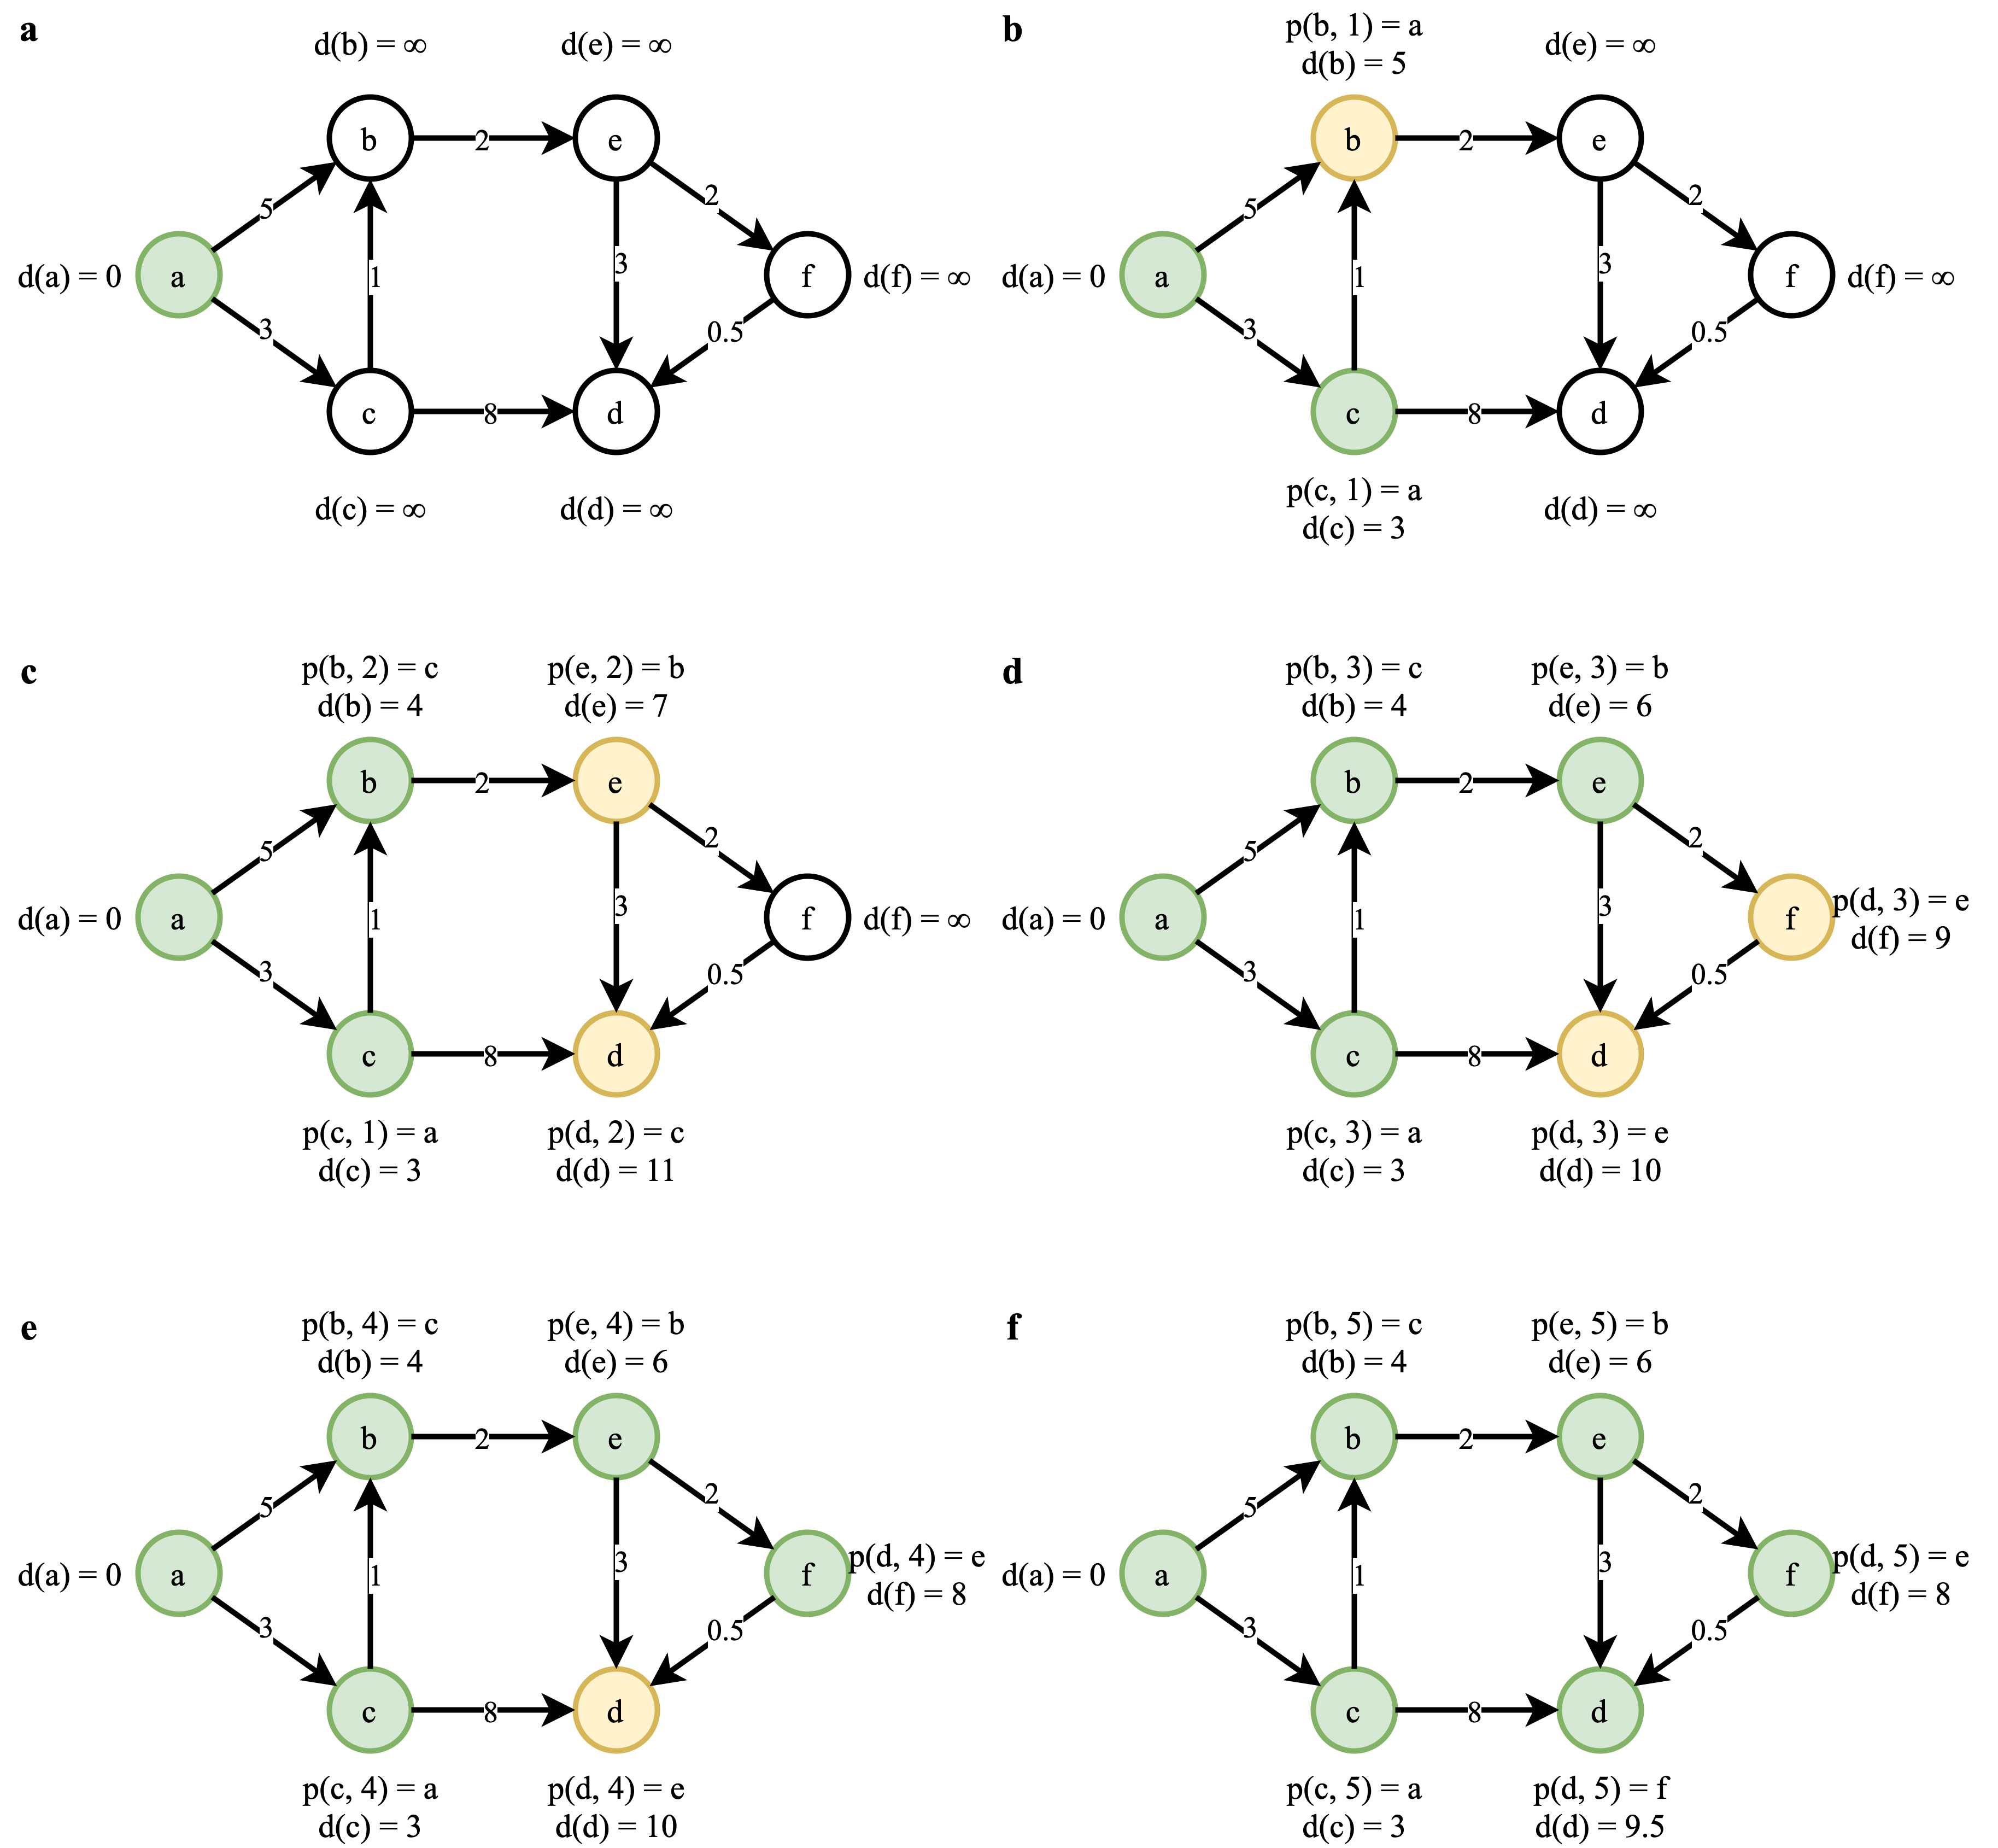
\includegraphics[width=1\textwidth]{./figures/ch3-bf.png}}
\caption{贝尔曼-福特算法示意图}
\label{fig-ch3-bf}
\end{figure}

贝尔曼-福特算法和迪杰斯特拉算法在结构上非常相似。迪杰斯特拉算法只查看每个节点的直连邻居节点,而贝尔曼-福特算法在每次迭代中都会遍历每条边。贝尔曼-福特算法的时间复杂度为:最佳情况下复杂度为$O(E)$;平均情况下复杂度$O(|V||E|)$;最坏情况下复杂度也是$O(|V||E|)$。空间复杂度为$O(V)$。贝尔曼-福特算法经常应用用于计算路由算法中的最短路径或者寻找最短路径,因此是非常适合用于本文对段路由航点计算的场景的。

2. 段列表生成算法

在计算了辅助图中每条链路的权重后,段列表生成算法将计算出尽力满足请求流量延迟要求的完整段路由标签列表。首先描述一下问题,假设网络中的所有节点都是段路由节点,并可能成为请求流量到达的段路由域的第一节点$s$或目的节点$t$。当前有一条流量的源节点和目的节点分别为$s$和$t$,并且需要有一个小于$d_{target}$的延迟。段列表生成算需要在网络存在动态流量的场景下构建段路由标签列表,使得通过这组段列表进行调度的流量有较大的可能实现端到端的时延尽量小,以至于时延小于目标值$d_{target}$。

贝尔曼-福特算法是基于松弛原理的。在每一步的计算中,最优权重路径逐渐被一个较小的新值所取代,直到最后达到最优解。从源节点到目的节点的非环形可达路径在图中最多有$|V|-1$边。贝尔曼-福特算法松弛了所有的链接,所以这个过程需要重复$|V|-1$次。该算法允许通过限制跳数来确定贝尔曼-福特算法是否需要继续。在每次迭代中,该算法将从源节点到目的节点的长度为$x+1$的路径的权重与上一次迭代中长度为$x$的路径的权重进行比较,并记录权重小于两者的路径。并更新最优路径。逐渐放宽路径长度,将得到从给定的源节点到目的节点的最优加权路径。

\subsection{算法时间复杂度分析}

在上述算法中,计算链路中心度的时间复杂度为$O(|V|log|V|+|E|)$,其中$k$为考虑的前$k$路径,$|V|$为节点数,$|E|$为边的数量。链接到达率和链接拥塞度可以直接采集或者通过时间复杂度为$O(1)$的方法计算得到,因此推导链接权重的时间复杂度可视为$O(|V|log|V|+|E|)$。计算辅助图的时间复杂度为$O({|V|}^{3/\alpha})$。然而,这两者都是由网络变化事件或定时器驱动的,因此在考虑段列表生成的时间复杂度时可以忽略。

基于贝尔曼-福特算法计算段路由列表的算法的时间复杂度为$O({|V|}^{3/\alpha})$,由于存在仅由${|V|}^\alpha$的节点组成的辅助图,因此时间复杂度降低。

\section{实验验证}

本小节将对上文提出的算法作出实验验证,实验将分别构建基于树形拓扑的数据中心网络拓扑和基于随机生成的运营商网络拓扑,并在这些拓扑中验证本节的算法和通过带宽选择航点的算法之间的的差异性。

\subsection{实验环境}

本实验使用第二代编程独立于协议的数据包处理器行为模型作为软件交换机。使用基于IPv6的段路由作为段路由标准而不是基于标签预留协议的段路由,因为IPv6是未来IP网络的趋势。而且基于IPv6的段路由使用128位的SID,更具有可扩展性。本实验使用Linux命名空间来隔离网络堆栈,使用虚拟以太网(Virtual Ethernet, veth)来模拟交换机之间的接口。基于IPv6的段路由程序用P4语言开发,在BMv2上加载实现,控制器的功能则由一个python进程来实现,整体实验架构如下图所示。

\begin{figure}[htbp]
\setlength{\abovecaptionskip}{15pt plus 3pt minus 2pt}
\centerline{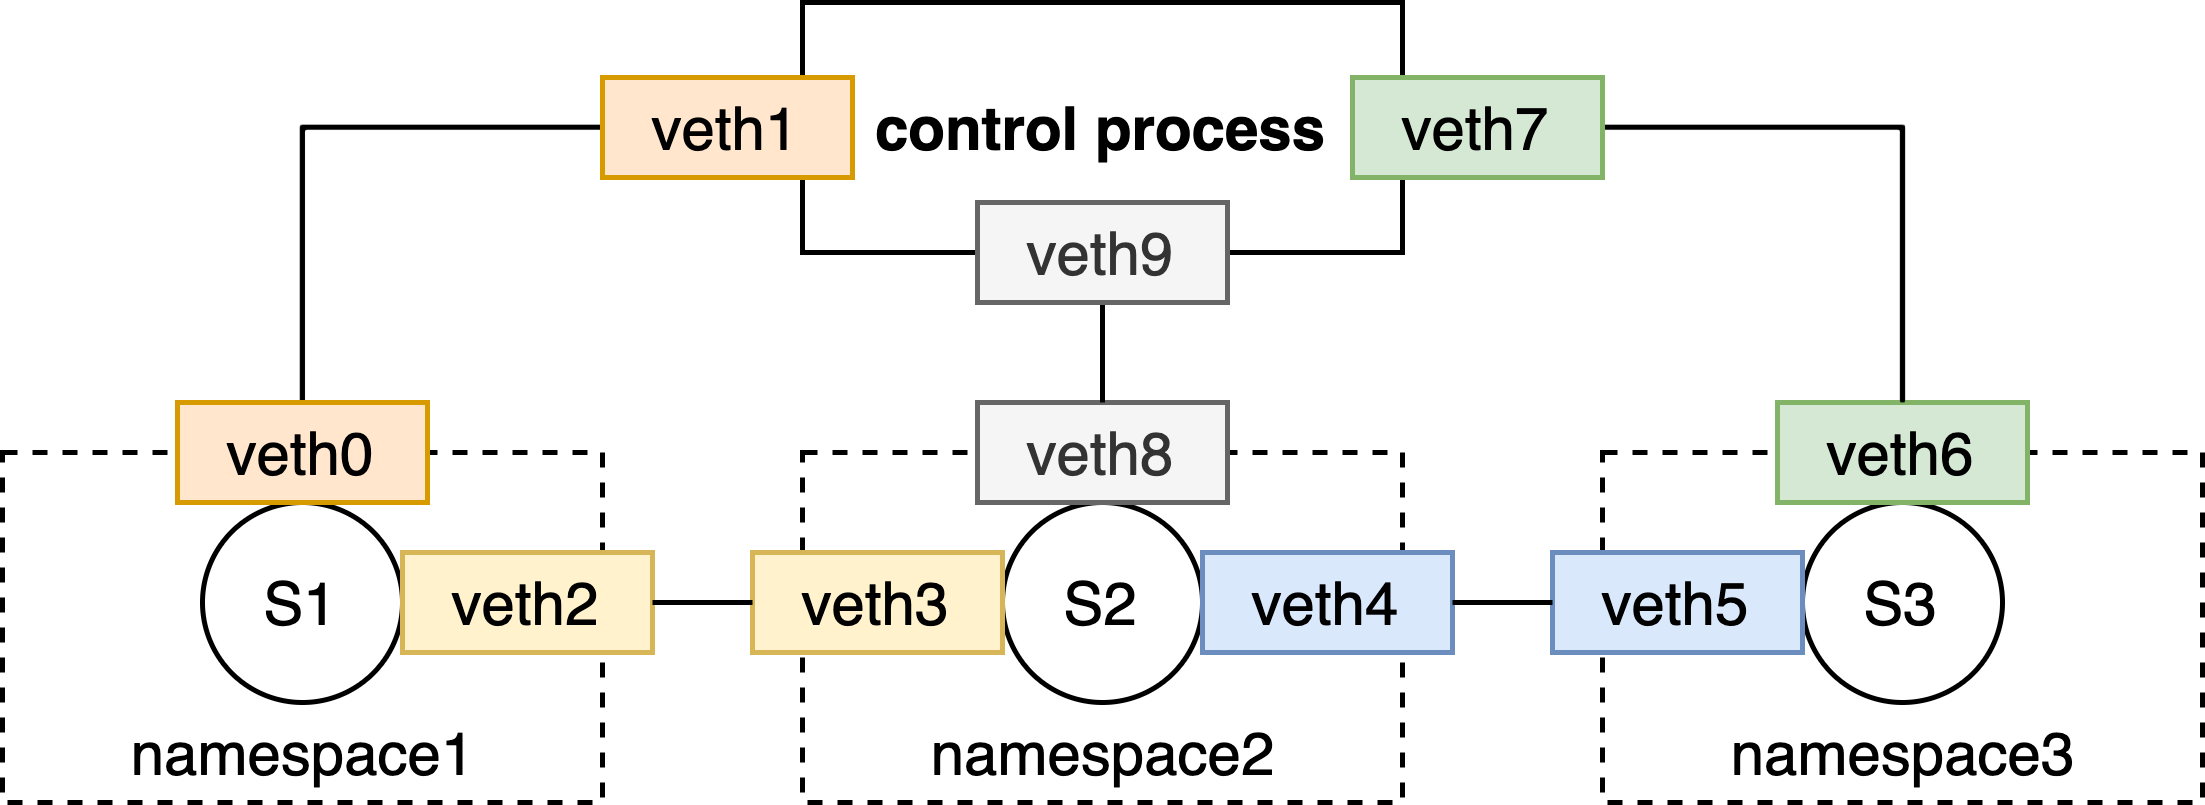
\includegraphics[width=0.8\textwidth]{./figures/ch3-test-env.png}}
\caption{实验环境示意图}
\label{fig-ch3-test-env}
\end{figure}

\subsection{实验步骤}

第一步启动网络拓扑,新建若干个网络命名空间,每一个网络命名空间相当于一个子网。将每对虚拟以太网绑定到对应的网络命名空间上并分配IPv4和IPv6地址。将设计好的拓扑中的每个虚拟交换机启动,加载编译的编程独立于协议的数据包处理器二进制文件,并的各个端口绑定到虚拟以太网上,这样在每对虚拟以太网间就形成连接两个虚拟交换机的链路。

第二步启动控制器,控制器将通过thrift接口和虚拟交换机BMv2建立带外通路进行控制流量传输。控制器将给所有虚拟交换机下发基础转发表项,包括二层广播表,等价多路径路由哈希组表,三层IPv6的路由器广告、邻居通告等代答表和三层IPv6路由表,使得全网拓扑中的节点可以用IPv6地址互通。

第三步在网络中选择两组相隔较远的节点,开始用流量生成软件Iperf持续性打流,保证在实验阶段网络处于有流量的动态状态。Iperf是一个用于网络性能测量和调优的工具。它是一种跨平台工具,可以为任何网络生成标准化的性能测量。Iperf具有客户端和服务器功能,并且可以创建数据流来测量两端之间的一个或两个方向的吞吐量。典型的 iperf 输出包含传输的数据量和测量的吞吐量的时间戳报告,本研究对时延结果数据的采集就是通过时间戳来获取。

第四步调整段路由航点选择算法参数,并启动段路由航点选择算法应用。

第五步选择一组源节点和目的节点开始从小流量开始打流,直到开始发生大规模的丢包,记录每次增加流量后控制器算法应用计算分配出的航点和端到端的时延情况。

第六步分析整理数据,得出结论。

\subsection{实验结果}

\begin{figure}[htbp]
\setlength{\abovecaptionskip}{15pt plus 3pt minus 2pt}
\centerline{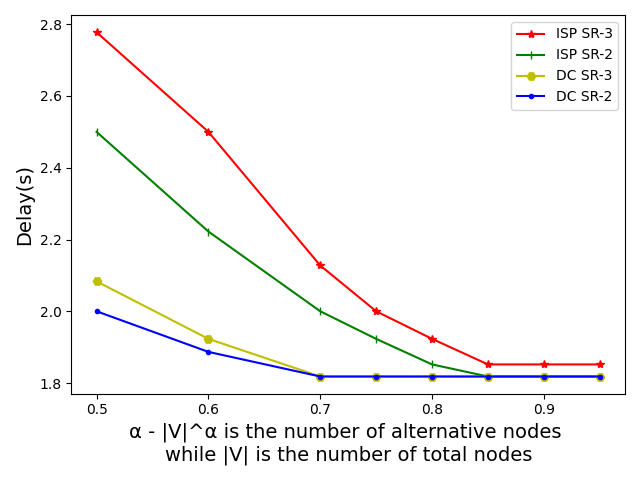
\includegraphics[width=0.8\textwidth]{./figures/ch3-test-1.png}}
\caption{$\alpha$取值测试结果图}
\label{fig-ch3-test-1}
\end{figure}

\begin{figure}[htbp]
\setlength{\abovecaptionskip}{15pt plus 3pt minus 2pt}
\centerline{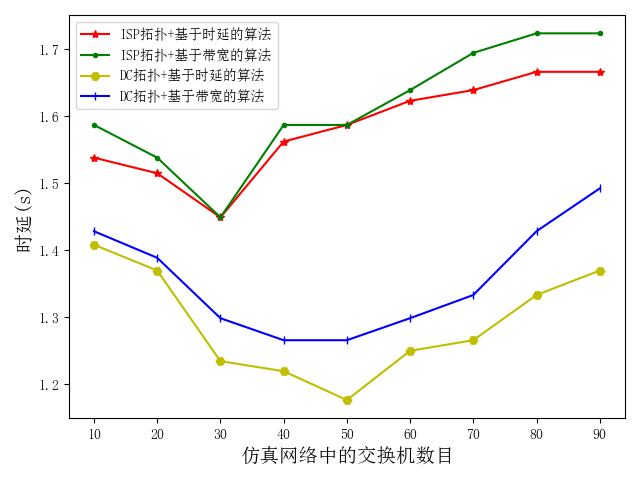
\includegraphics[width=0.8\textwidth]{./figures/ch3-test-2.png}}
\caption{平均延迟实验结果图}
\label{fig-ch3-test-2}
\end{figure}

\begin{figure}[htbp]
\setlength{\abovecaptionskip}{15pt plus 3pt minus 2pt}
\centerline{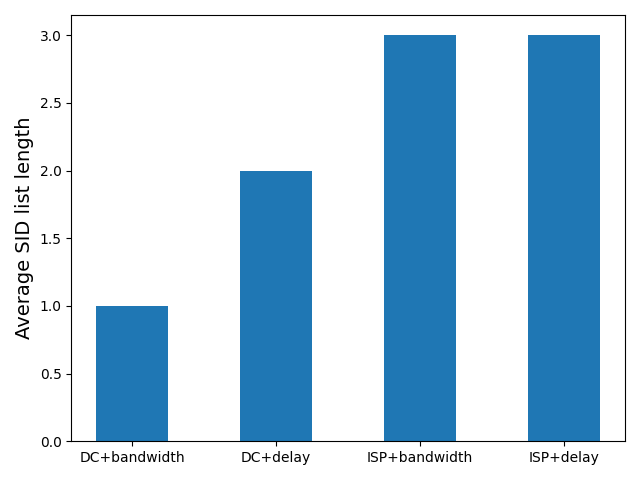
\includegraphics[width=0.8\textwidth]{./figures/ch3-test-3.png}}
\caption{标签列表长度实验结果图}
\label{fig-ch3-test-3}
\end{figure}

\begin{figure}[htbp]
\setlength{\abovecaptionskip}{15pt plus 3pt minus 2pt}
\centerline{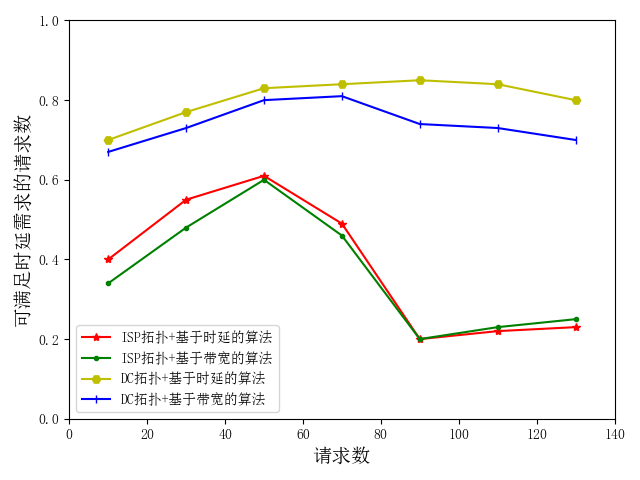
\includegraphics[width=0.8\textwidth]{./figures/ch3-test-4.png}}
\caption{保证请求延迟要求比例测试结果图}
\label{fig-ch3-test-4}
\end{figure}

1. $\alpha$取值测试

图3-a是为了验证候选节点占原拓扑全部节点的比率$\alpha$的取值。该试验将选择两个拓扑,一个是数据中心的树状拓扑结构,一个是随机生成的互联网服务提供商(ISP)拓扑。两个拓扑都具有40个节点;另外分别将段路由标签列表限制为2跳或3跳,即$SR-2$和$SR-3$。每一次确定参数$\alpha$的取值后后按照实验步骤3开始打流,记录iperf打流的时延结果。图中横轴是$\alpha$的大小,纵轴是延迟。

在数据中心的树状拓扑结构中,根据$SR-2$、$SR-3$进行比较,同时调整$\alpha$的值。可以看出,当选择$\alpha=0.7$时,在数据中心场景中SR-2和SR-3的情况下可以达到最佳值。其含义是:当节点集中有节点中心度在前${|V|}^{0.7}$的节点时。需要在计算中考虑时,已经可以得到效果最优的分段路由路径。而在互联网服务提供商拓扑中,使用随机拓扑进行模拟,在$SR-2$和$SR-3$的情况下,$\alpha=0.85$可以达到最优值。

2. 平均延迟实验

图3-b是为了验证在同样使用贝尔曼-福特算法作为标签列表选择核心算法的前提下,采用本文提出的链路权重以及生成辅助图的方案和直接用链路带宽作为权重的方案进行比较。实验的对照组同样是数据中心的树状拓扑结构和随机生成的互联网服务提供商拓扑。本实验的自变量是网络的大小,用网络拓扑中的交换机数目,即节点数目做为横坐标,因变量是打流的时延结果,并将其在纵坐标上描点,进而分析得出结论。如图3-b表明,当使用考虑时延的链路权重进行段路由标签列表计算时,无论使用树状拓扑结构还是随机拓扑结构,相对于直接使用带宽信息来计算来段列表,都能获得更低的平均延迟。

3. 标签列表长度实验

图3-c是为了验证3.3.1中提到的用段路由标签列表的长度被用来限制段列表生成算法,在数据中心的树状拓扑结构和互联网服务提供商随机拓扑结构中,分别使用了本文提出的基于带宽的贝尔曼-福特算法,以及本文提出的参考延迟的贝尔曼-福特算法。对四种场景下生成的段路由标签列表的平均列表长度进行比较。横坐标是四种测试场景,纵坐标是段标签列表的长度。本文提出的算法倾向于使用稍大的段列表长度,但考虑到贝尔曼-福特算法在生成段列表长度的时候会对长度进行限制,所以可以通过约束条件来保障段标签列表长度不会太长。本文使用的段标签列表都是2个或3个,因此可以认为没有产生额外的段列表标签开销。

4. 保证请求延迟要求比例测试

图3-d是为了验证使用本文提出的参考时延属性的段路由标签列表生成算法是否可以对时延需求进行保障。本实验的对比拓扑还是树状拓扑和互联网服务提供商拓扑,分别使用本文提出的参考延迟的贝尔曼-福特算法和基于带宽的贝尔曼-福特算法来计算给定服务请求数在10、50、90、130的情况下,可以分别保证请求延迟要求的比例。横坐标自变量是发起请求的数目,在实验中是从不同的源地址到目的地址进行打流,查看该流量被调度后的时延是否符合目标时延的需求,即实际时延小与目标时延,对满足时延需求的请求进行计数,与总请求数的比例就是纵坐标的数据。到可以看出,无论在树状拓扑结构还是互联网服务提供商拓扑中,本研究提出的算法都具有更好的延迟保证效果。

\section{算法结论}

在本章节中设计了一种参考链路时延构建链路权重选择段路由段列表的算法。该算法从多个角度测量并分析数据特性和研究的模型需求构成链路权重计算公式,通过对集中网络节点介数中心度进行分析得出用更少节点构建辅助图的拓扑降维方案,并使用贝尔曼-福特算法来推导计算出段列表。3.4的实验部分证明了该算法在时延保障上具有一定的有效性。

本文的算法仍有一些不足之处,例如,链路到达率是一个相当理想的值,在现实的网络中可能很难使用。此外,带内遥测的准确性会影响算法的结果,目前在商业交换机中,带内遥测数据是每3秒或10秒收集一次。因此,未来的工作是研究如何在算法中有效地收集和计算每个参数,并在物理网络中验证该算法。

\chapter{基于差分时延的分布式路径选择算法}

\section{引言}

在上一章提出的算法中,集中式的段路由路径选择算法具有全局调优,资源协调整合的优点,但是在面对网络流量动态变化频繁,对服务质量的实效性要求较强的的时候,集中式的控制计算方式就会产生较大的处理延迟,因此本章将从分布式的角度对段路由的时延需求进行保障。

除了计算时延需求的段路由航点的分布式优化外,上一章提出的算法只能尽力保障业务流量的时延更低,但是对于业务提出的明确时延需求并没有针对地进行资源分配,这主要是因为时延的资源计算更为复杂,无法像计算剩余带宽一样直接减去使用带宽,并且先到先服务的尽力而为架构在一定程度上也是可以保障互联网的公平性。但是对于需要差分服务质量的网络,这种方案就不太可行。因此为了对时延服务质量需求进行更有针对性的资源分配,本章将用对时延进行差分分组的方式设计分布式保障时延需求的算法。

本章将对基于时延的路径选择算法进行建模分析、算法阐释,并给出实验验证结果。本文参考边界网关协议的实现逻辑,考虑在航点之间如何进行数据交互以及使用怎样的分布式算法可以计算得到具有最好的时延保障效果的段路由航点列表。与第三章侧重点的不同主要在于,第三章的算法是控制器运行的算法,而第四章的算法主要是数据面分布式的协议和算法。

\section{问题模型}

在广域网的路由系统中,按照规划或地域原因往往被分为很多的自治域(Autonomous system, AS),自治域内部使用内部网关协议进行内部通信,自治域之间使用边界网关协议进行跨域通信,整个网络中的网元节点要运行内部网关协议、边界网关协议等路由协议来保证网络内部节点的互相连通性,这些协议也会随着网络动态变化实时更新网络交换机的路由信息表,多种类型的路由表信息经过一定的算法整合就将生成转发信息库 (FIB),当交换机收到一个新的数据包时,它会直接通过查找转发信息库将数据包转发到正确的端口,最终实现全网路由可达。当段路由运行在广域网中时,广域网的路由系统会被类似地划分为很多的分段路由域用于对标签进行管理,通常也不要求所有网元节点都支持段路由功能,而是部分节点具有封装、传递、弹出段路由报文头的功能即可,如图4-1所示。因此这些具有段路由功能的网元节点实际上组成了一张节点数和链路数更少的段路由网络。

\begin{figure}[htbp]
\setlength{\abovecaptionskip}{15pt plus 3pt minus 2pt}
\centerline{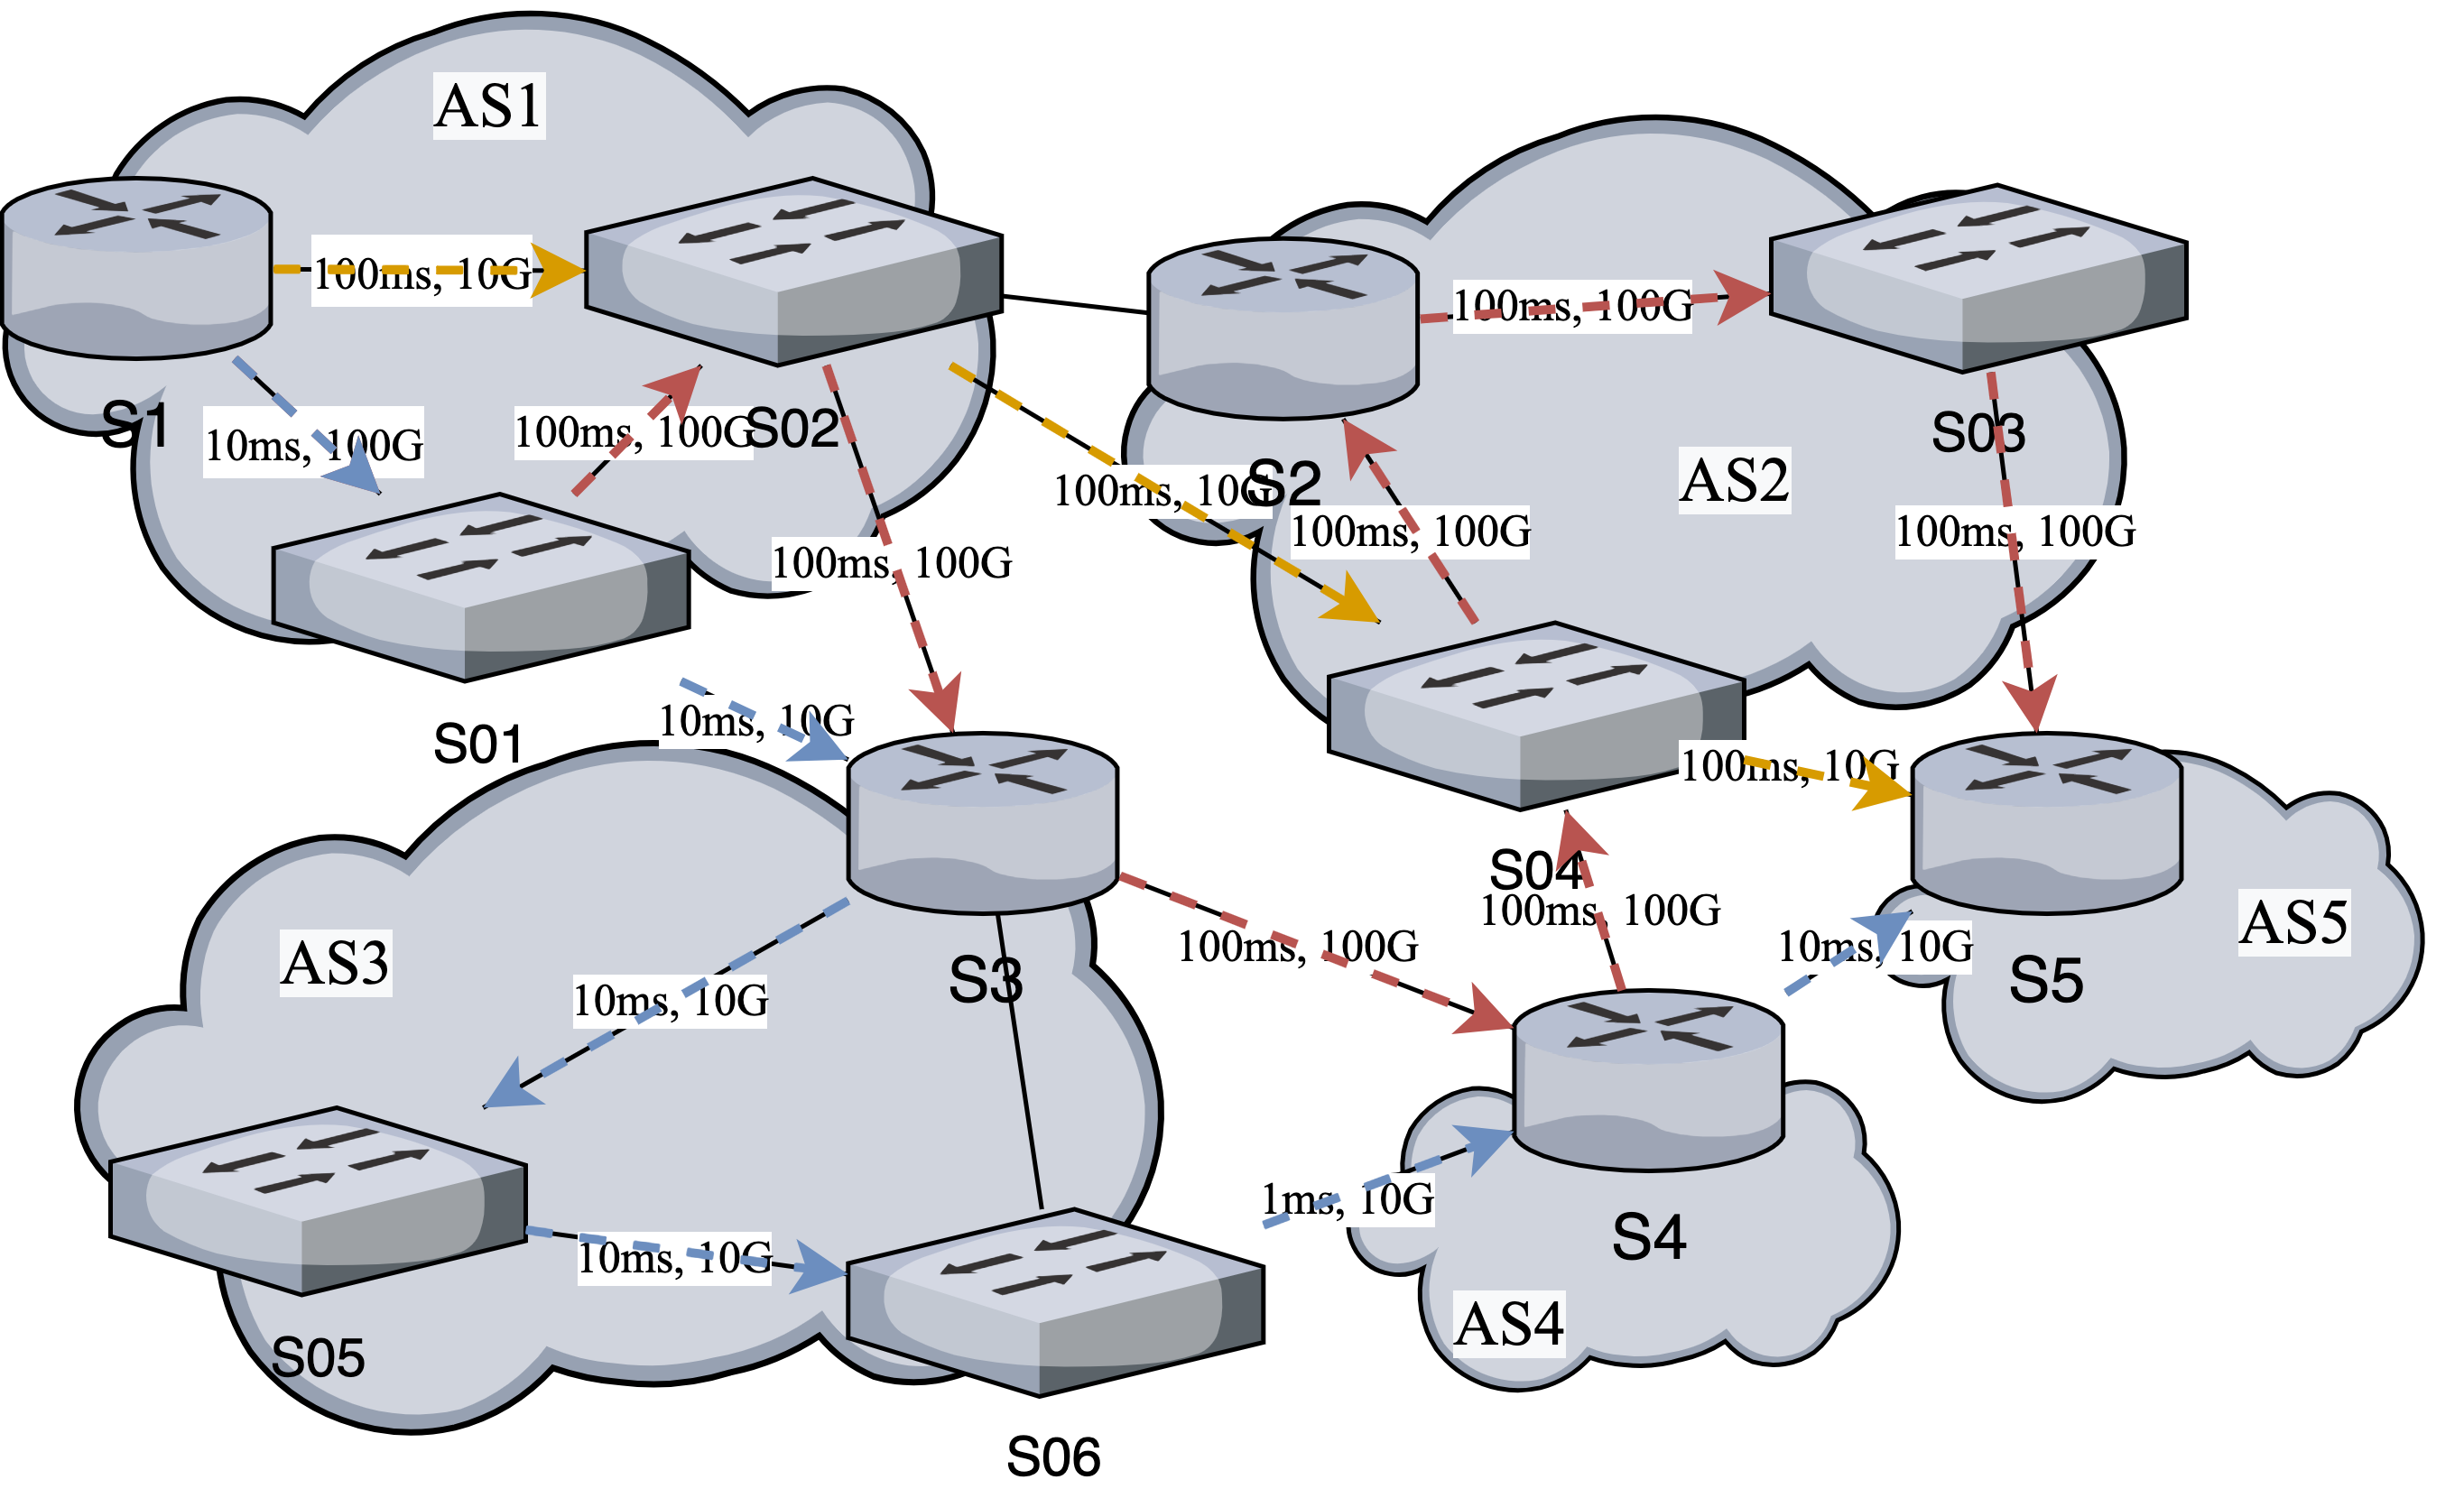
\includegraphics[width=1\textwidth]{./figures/ch4-problem-model.png}}
\caption{分布式段路由选路方案示意图}
\label{fig-ch4-problem-model}
\end{figure}    

端到端报文在到达某个段路由交换机时是从一个段路由域内去往另一个段路由域,并且携带一个目标时延,入口段路由节点就会按照本地的段路由策略选择合适的段路由标签列表,并封装到报文头部指导转发路径。假设段路由策略被配置为按照最短跳数选择路径。如图4-1所示,则在AS1中,目的地址在AS5中的数据包都将沿着图中黄色路径(AS1(S1 -> S02) -> AS2(S04) -> AS5(S5))转发;如果按照带宽选择路径,目的地址在AS5中的数据包都将沿着图中红色路径(AS1(S1 -> S01 -> S02) -> AS3(S3) -> AS4(S4) -> AS2(S04 -> S2 -> S03) -> AS5(S5))转发;而如果按照时延选择路径,目的地址在AS5中的数据包都将沿着图中蓝色路径(AS1(S1 -> S01) -> AS3(S3 -> S05 -> S06) -> AS4(S4) -> AS5(S5))转发。

因此将网络拓扑图抽象为以全部网络节点为点集合,以全部链路为双向有向链路边集合的有向图,将适配流量所需时延作为优化目标构建数学模型,待求解对象为段路由节点内对其他节点进行时延表达的数据结构以及匹配目标时延的方法。用公式表达如下:
$$min(\frac{|D_{target}-D_{redult}|}{D_{target}})$$

\section{差分时延多路径路由算法}

\subsection{算法概述}

差分时延的路径选择算法是一个分布式算法,任何段路由节点都需要参与其中。在差分时延的路径选择算法中,每个段路由节点内部维护一个差分时延段路由策略表,并通过ICMP协议获取本段路由节点到其余段路由节点的由传统路由系统计算得出的的默认路径的时延,记录这个时延是有意义的,因为当数据包从一个航点到下一个航点,一定是通过传统的基础分布式路由算法得到的选路结果。这些段路由节点间的时延将被类似边界网关协议宣告的方式传达给其他段路由节点,每个段路由节点将收到的消息更新在自己的差分时延段路由策略表。这部分算法和差分时延段路由策略表的数据结构将在4.3.4进行详细梳理。当这些测量结果在全网的段路由节点处整合收敛,网络中就形成了分布式的段路由节点优选差分时延矩阵。矩阵的规划和数据属性将在4.3.2进行分析。因此各个段路由节点就可以利用这些测量结果找到一对段路由节点之间的多条可达路径,且具有段路由节点之间路径的时延信息,即差分时延矩阵。在多条可达路径中,存在各种差分分组的时延,如1ms-10ms级、10ms-100ms级、100ms-1s级、1s-10s级等,这些时延信息将被段路由节点以时延矩阵的方式进行分类。当服务流量到达一个段路由节点的时候,就将对待服务流量的需求时延落入分级的差分分组中,并使用组内的段路由实现方案进行递归路径选择,并最终生成段路由航点列表,选择的结果将基于流量的五元组哈希和段路由方案的惩罚值,这部分内容将在4.3.5段路由航点列表生成算法中进行分析,本节算法思路的结构索引如图4-2所示。

\begin{figure}[htbp]
\setlength{\abovecaptionskip}{15pt plus 3pt minus 2pt}
\centerline{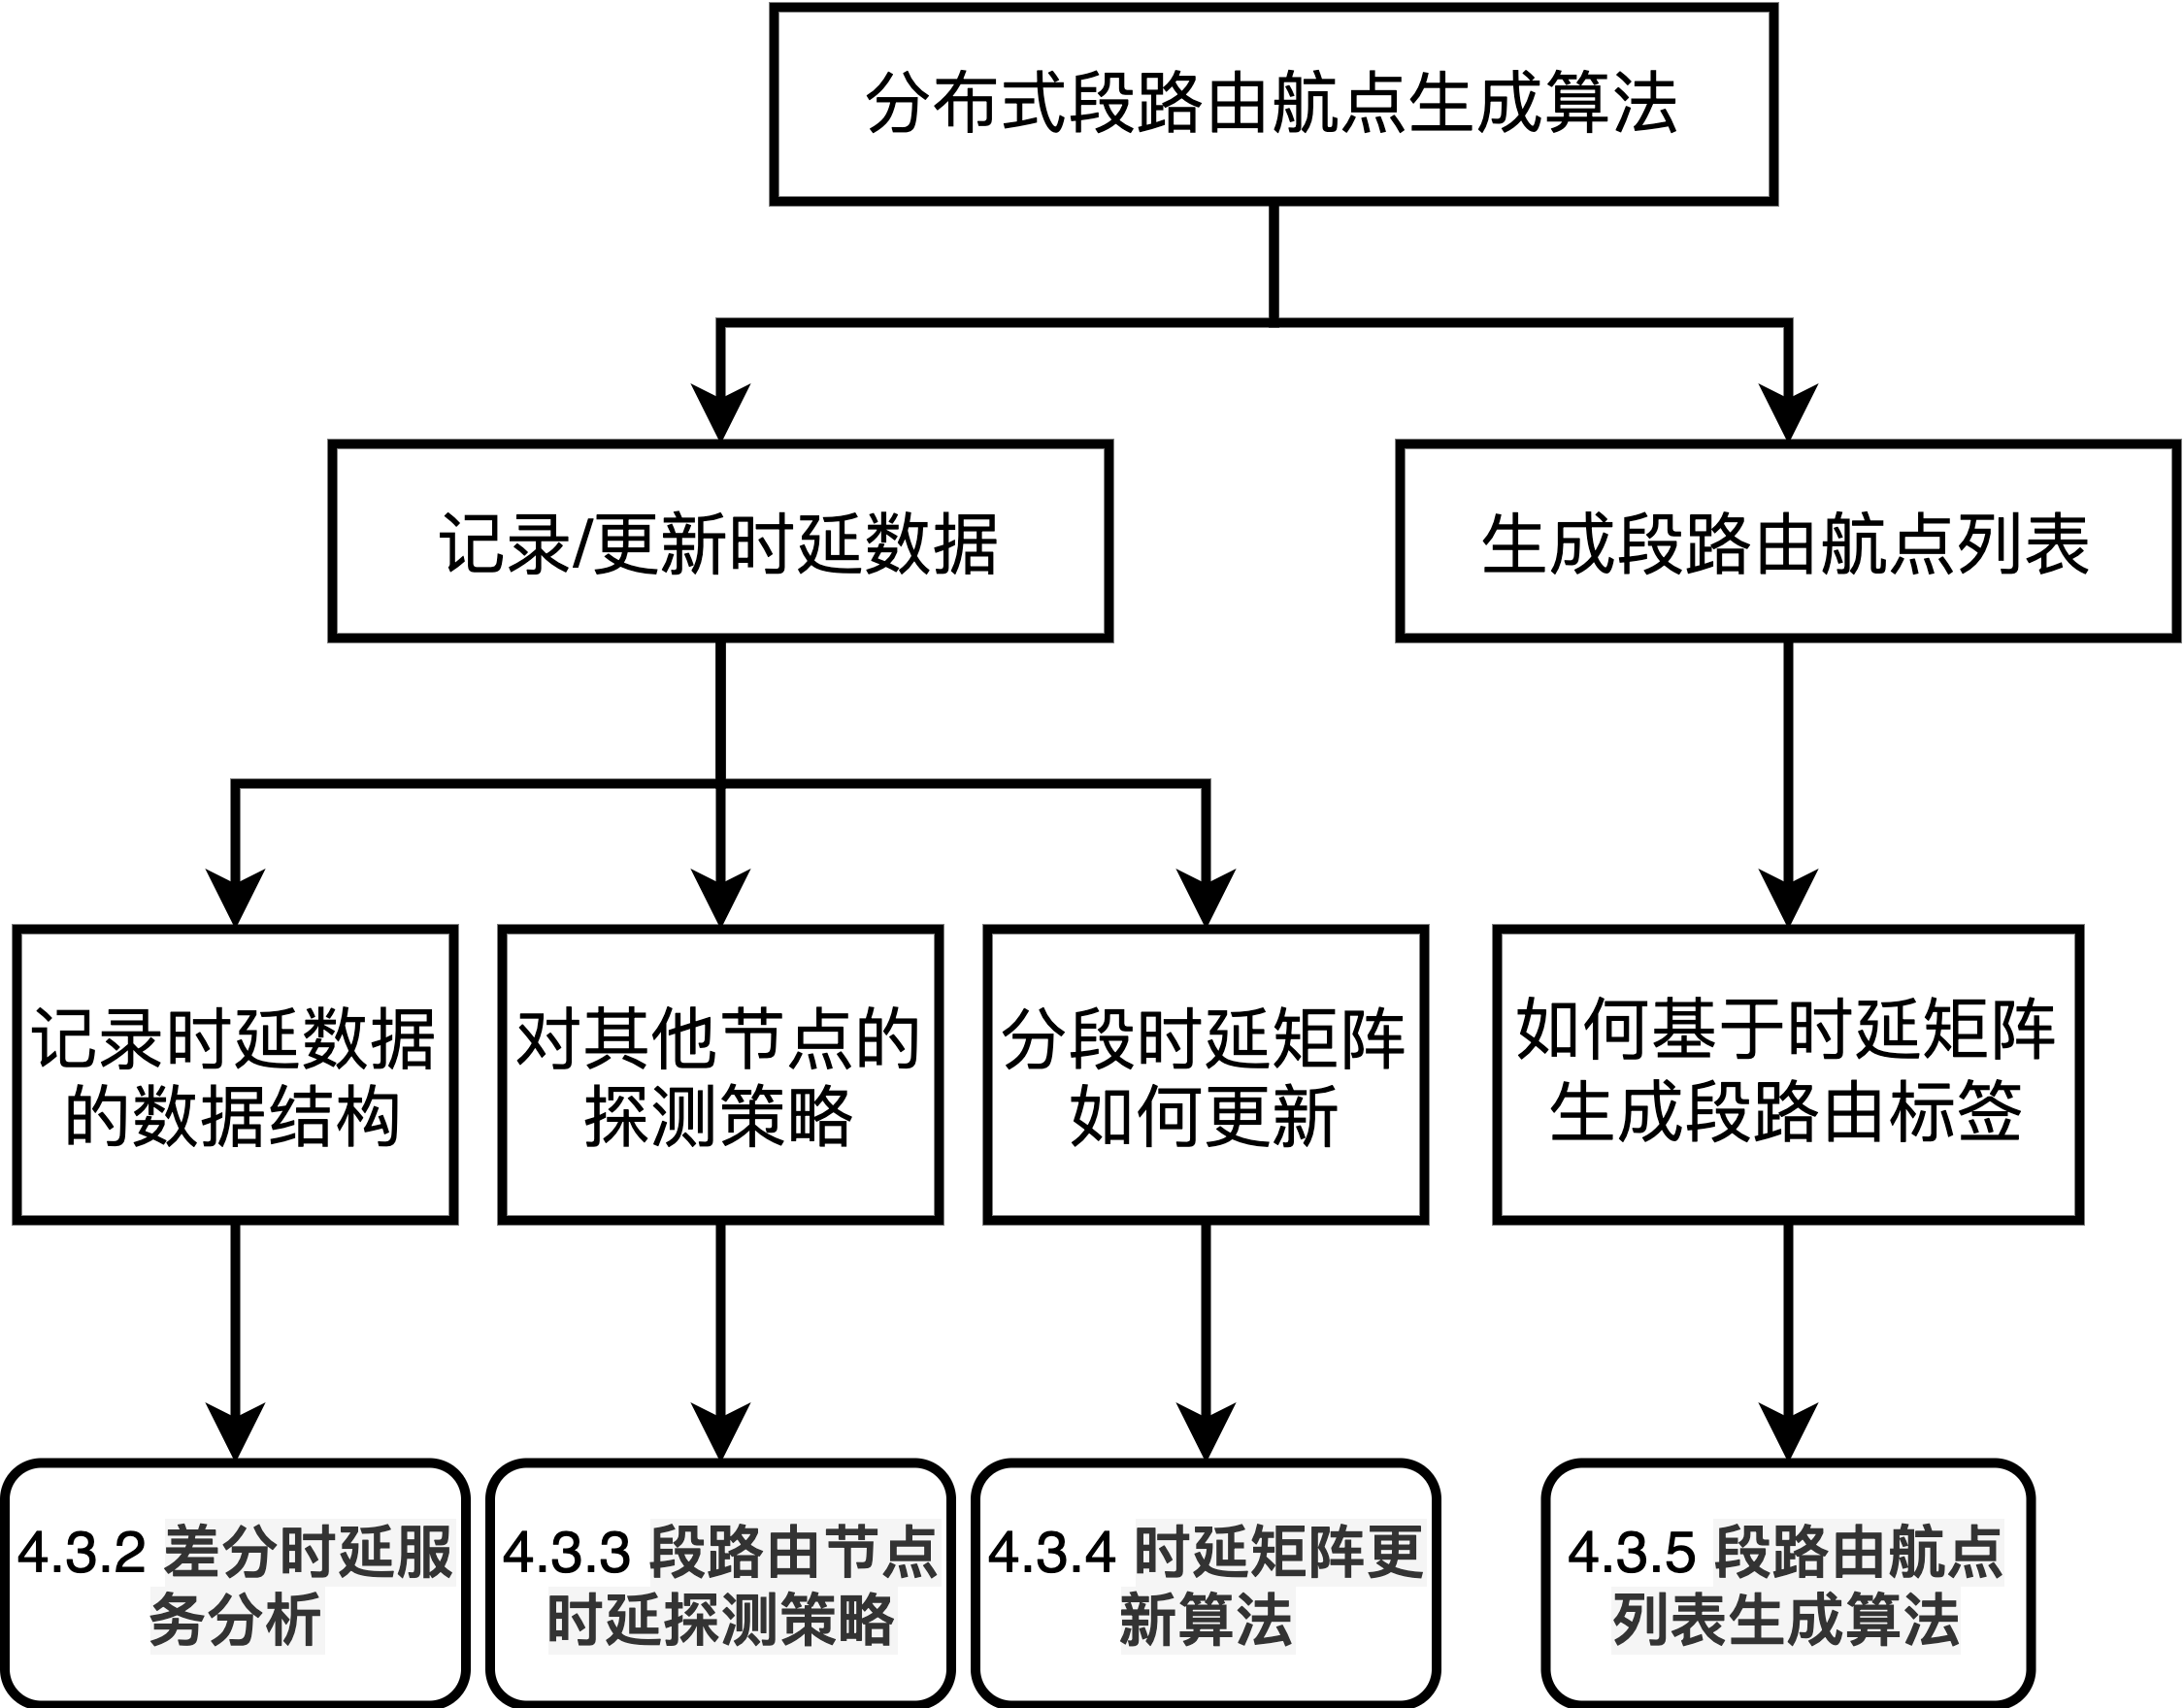
\includegraphics[width=0.8\textwidth]{./figures/ch4-ark.png}}
\caption{分布式段路由航点列表生成算法思路索引结构图}
\label{fig-ch4-ark}
\end{figure}

本章的算法主要有以下几个挑战:

\begin{itemize}
\item 挑战1:对于每一台交换机,时延探测的对象有谁?该挑战需要明确时延探测对象是因为如果选择探测全体其他段路由节点会造成过大的探测流量影响网络的吞吐,而过小的探测对象数目可能导致探测结果的不全面,无法得到时延最短的路径。
\item 挑战2:每个交换机需要以怎样的数据结构存储与其他段路由之间的时延信息可以做到占用较少的资源实现较高的效率?这是由于对于每一台运行路径选择算法的交换机都需要维护一张与其他组交换机间时延的表,段路由节点过多和时延分组的过多会导致表格以乘法关系的增长,这会造成比较大的数据冗余,因此需要设计更为合理的存储段路由节点间时延信息的数据结构。
\item 挑战3:怎样的时延矩阵更新方式可以更好得保障时延信息的及时性并且破坏稳定性?这个挑战的存在是由于类似路由翻滚的情况也有可能发生在段路由航点列表的算法结果选择上,本章希望可以得到一个抑制无效段路由航点列表计算结果翻滚的方案来降低相同时延需求和源、目的地址流量计算出的段路由列表方案来回切换的可能。
\end{itemize}

\subsection{差分时延服务分析}

段路由节点之间的时延根据段路由节点的地理位置会出现很大的差异,例如从国内一个可用区的数据中心中的两个段路由节点之间测量时延,大概仅有1毫秒的时延,这是因为同一数据中心由于其风和水电统一规划、地理位置比较接近,光线行程较短,因此时延很低,一般对时延需求很高的业务也会部署在同一个可用区测数据中心中;如果测量国内两个可用区之间的不同段路由节点之间时延,其时延大致在10毫秒的量级;而如果从国内到国外的两个段路由节点之间测量时延,大概会到100毫秒左右。这是因为[XX]研究认为互联网的往返时延即RTT随着互联网上数据分组从源节点到目的端经过的中转路由器的个数增加而增加,即往返时延与本文所定义的段路由通信跳数成正比。研究[XX]得出链路两端距离小于5000千米的主要发生时延主要由排队时延组成,而链路两端距离大于5000千米的主要发生时延主要由传播时延组成的结论,综上所述,段路由节点之间的地理位置差异造成了彼此间通信的时延差异。

段路由节点会按照4.3.3描述的规则对其他段路由节点进行时延探测,时延探测结果被分成几类,每个段路由节点维护一个本节点到所有备选段路由节点组的时延记录数据结构,首先按照差分时延分段的机制,将目标时延分成几个区间,1毫秒到10毫秒,10毫秒到100毫秒,100毫秒到1秒…,在段路由节点中存储的数据结构如下表所示:

\begin{table}[]
\begin{tabular}{|p{0.2\textwidth}|p{0.7\textwidth}|}
\hline
1毫秒到10毫秒 & {[}SR目的节点1:\{下一跳SR节点组1, 总时延1\}, SR目的节点2:\{下一跳SR节点组2, 总时延2\}, ...{]} \\ \hline
10毫秒到100毫秒 & {[}SR目的节点3:\{下一跳SR节点组3, 总时延3\}, ...{]} \\ \hline
100毫秒到1秒 & {[}SR目的节点4:\{下一跳SR节点组4, 总时延4\}, ...{]} \\ \hline
... &  \\ \hline
\end{tabular}
\caption{节点时延矩阵结构图}
\label{table-delay-metric}
\end{table}

其中SR目的节点以哈希集合方式存储,目的节点对应的段路由方案列表用优先级队列存储,即队首时延最低,逐次递增。

\begin{figure}[htbp]
\setlength{\abovecaptionskip}{15pt plus 3pt minus 2pt}
\centerline{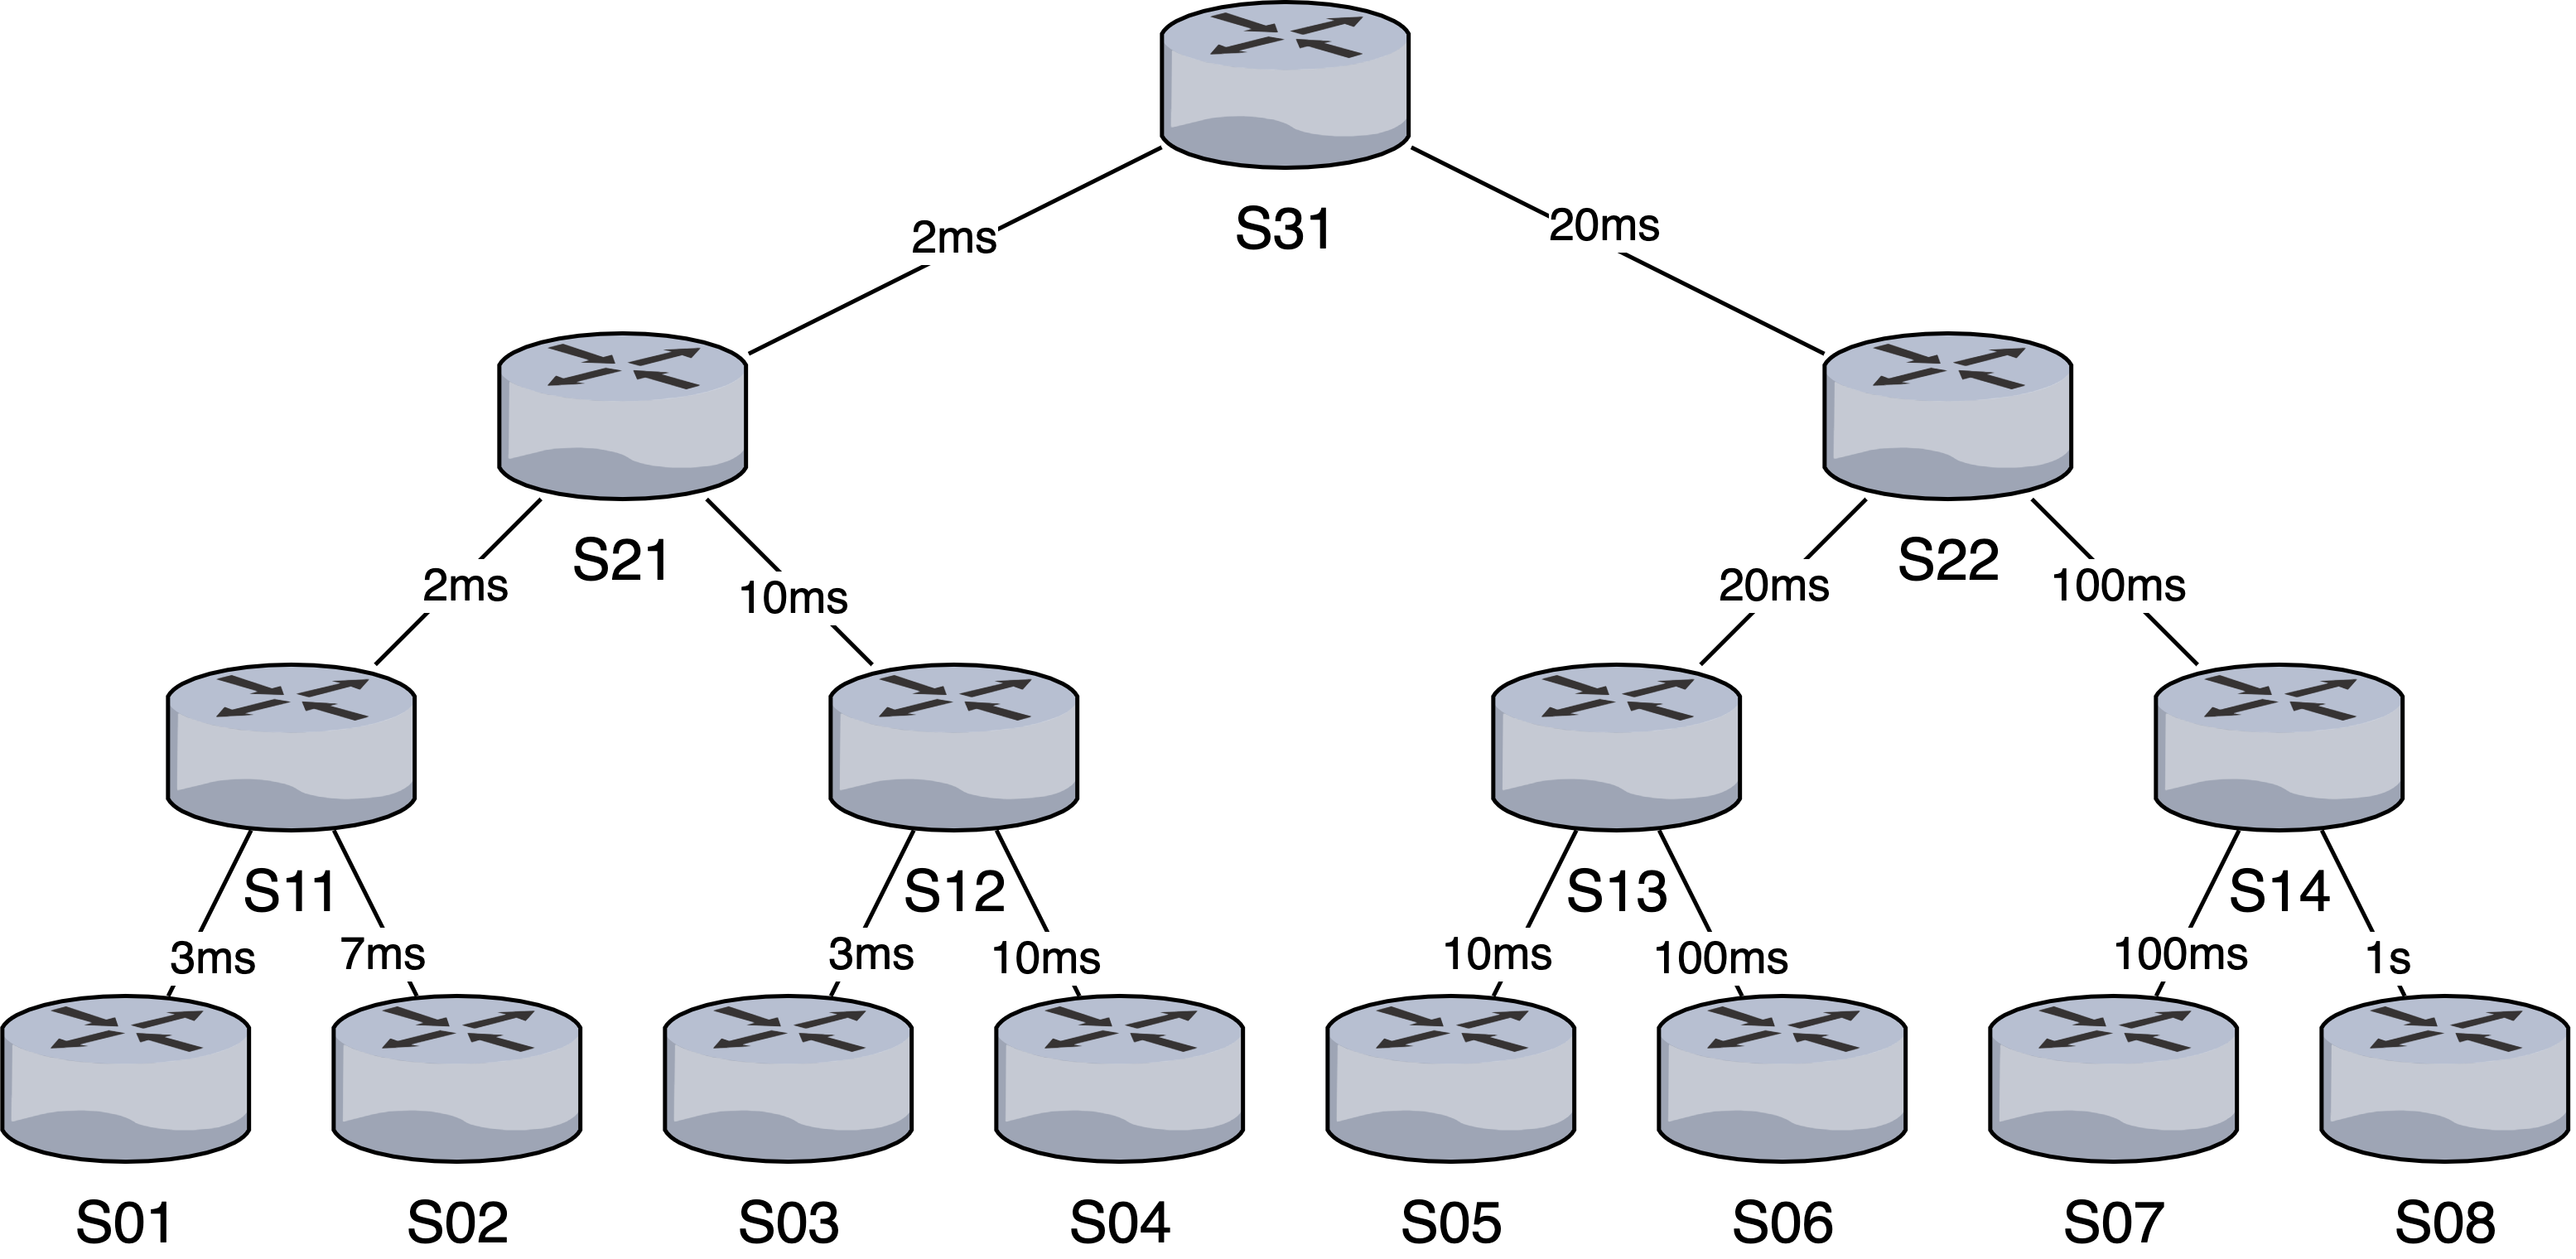
\includegraphics[width=0.8\textwidth]{./figures/ch4-tree-topo.png}}
\caption{段路由差分分组时延矩阵示意拓扑图}
\label{fig-ch4-tree-topo}
\end{figure}

以10毫秒到100毫秒的时延区间为例,如上图所示,$S_{31}$的段路由节点可以得到如下表的时延采集记录。

\begin{table}[htbp]
\begin{tabular}{|p{0.2\textwidth}|p{0.7\textwidth}|}
\hline
1毫秒到10毫秒 & {[}S21:\{nil, 2ms\}, S11:\{S21, 4ms\}{]} \\ \hline
10毫秒到100毫秒 & {[}S22:\{nil, 20ms\}, S12:\{S21, 12ms\}, S13:\{nil, 40ms\}{]} \\ \hline
100毫秒到1秒 & {[}S14:\{S22, 120ms\}{]} \\ \hline
\end{tabular}
\caption{节点时延矩阵填写示意图}
\label{table-fullin-delay-metric}
\end{table}

\subsection{段路由节点时延探测策略}

每个段路由节点在选择需要探测的节点列表时有一些潜在的问题。如果让每个节点探测所有其他节点就会造成高带宽开销的代价;而如果让每个节点随机探测一组节点就无法保证任何节点对的两个探测集的交集是非空的,即不能保证每个节点都被探测到。因此本节会提出一种可以较为公平探测段路由节点的算法,并且造成较小的带宽费用。

\begin{figure}[htbp]
\setlength{\abovecaptionskip}{15pt plus 3pt minus 2pt}
\centerline{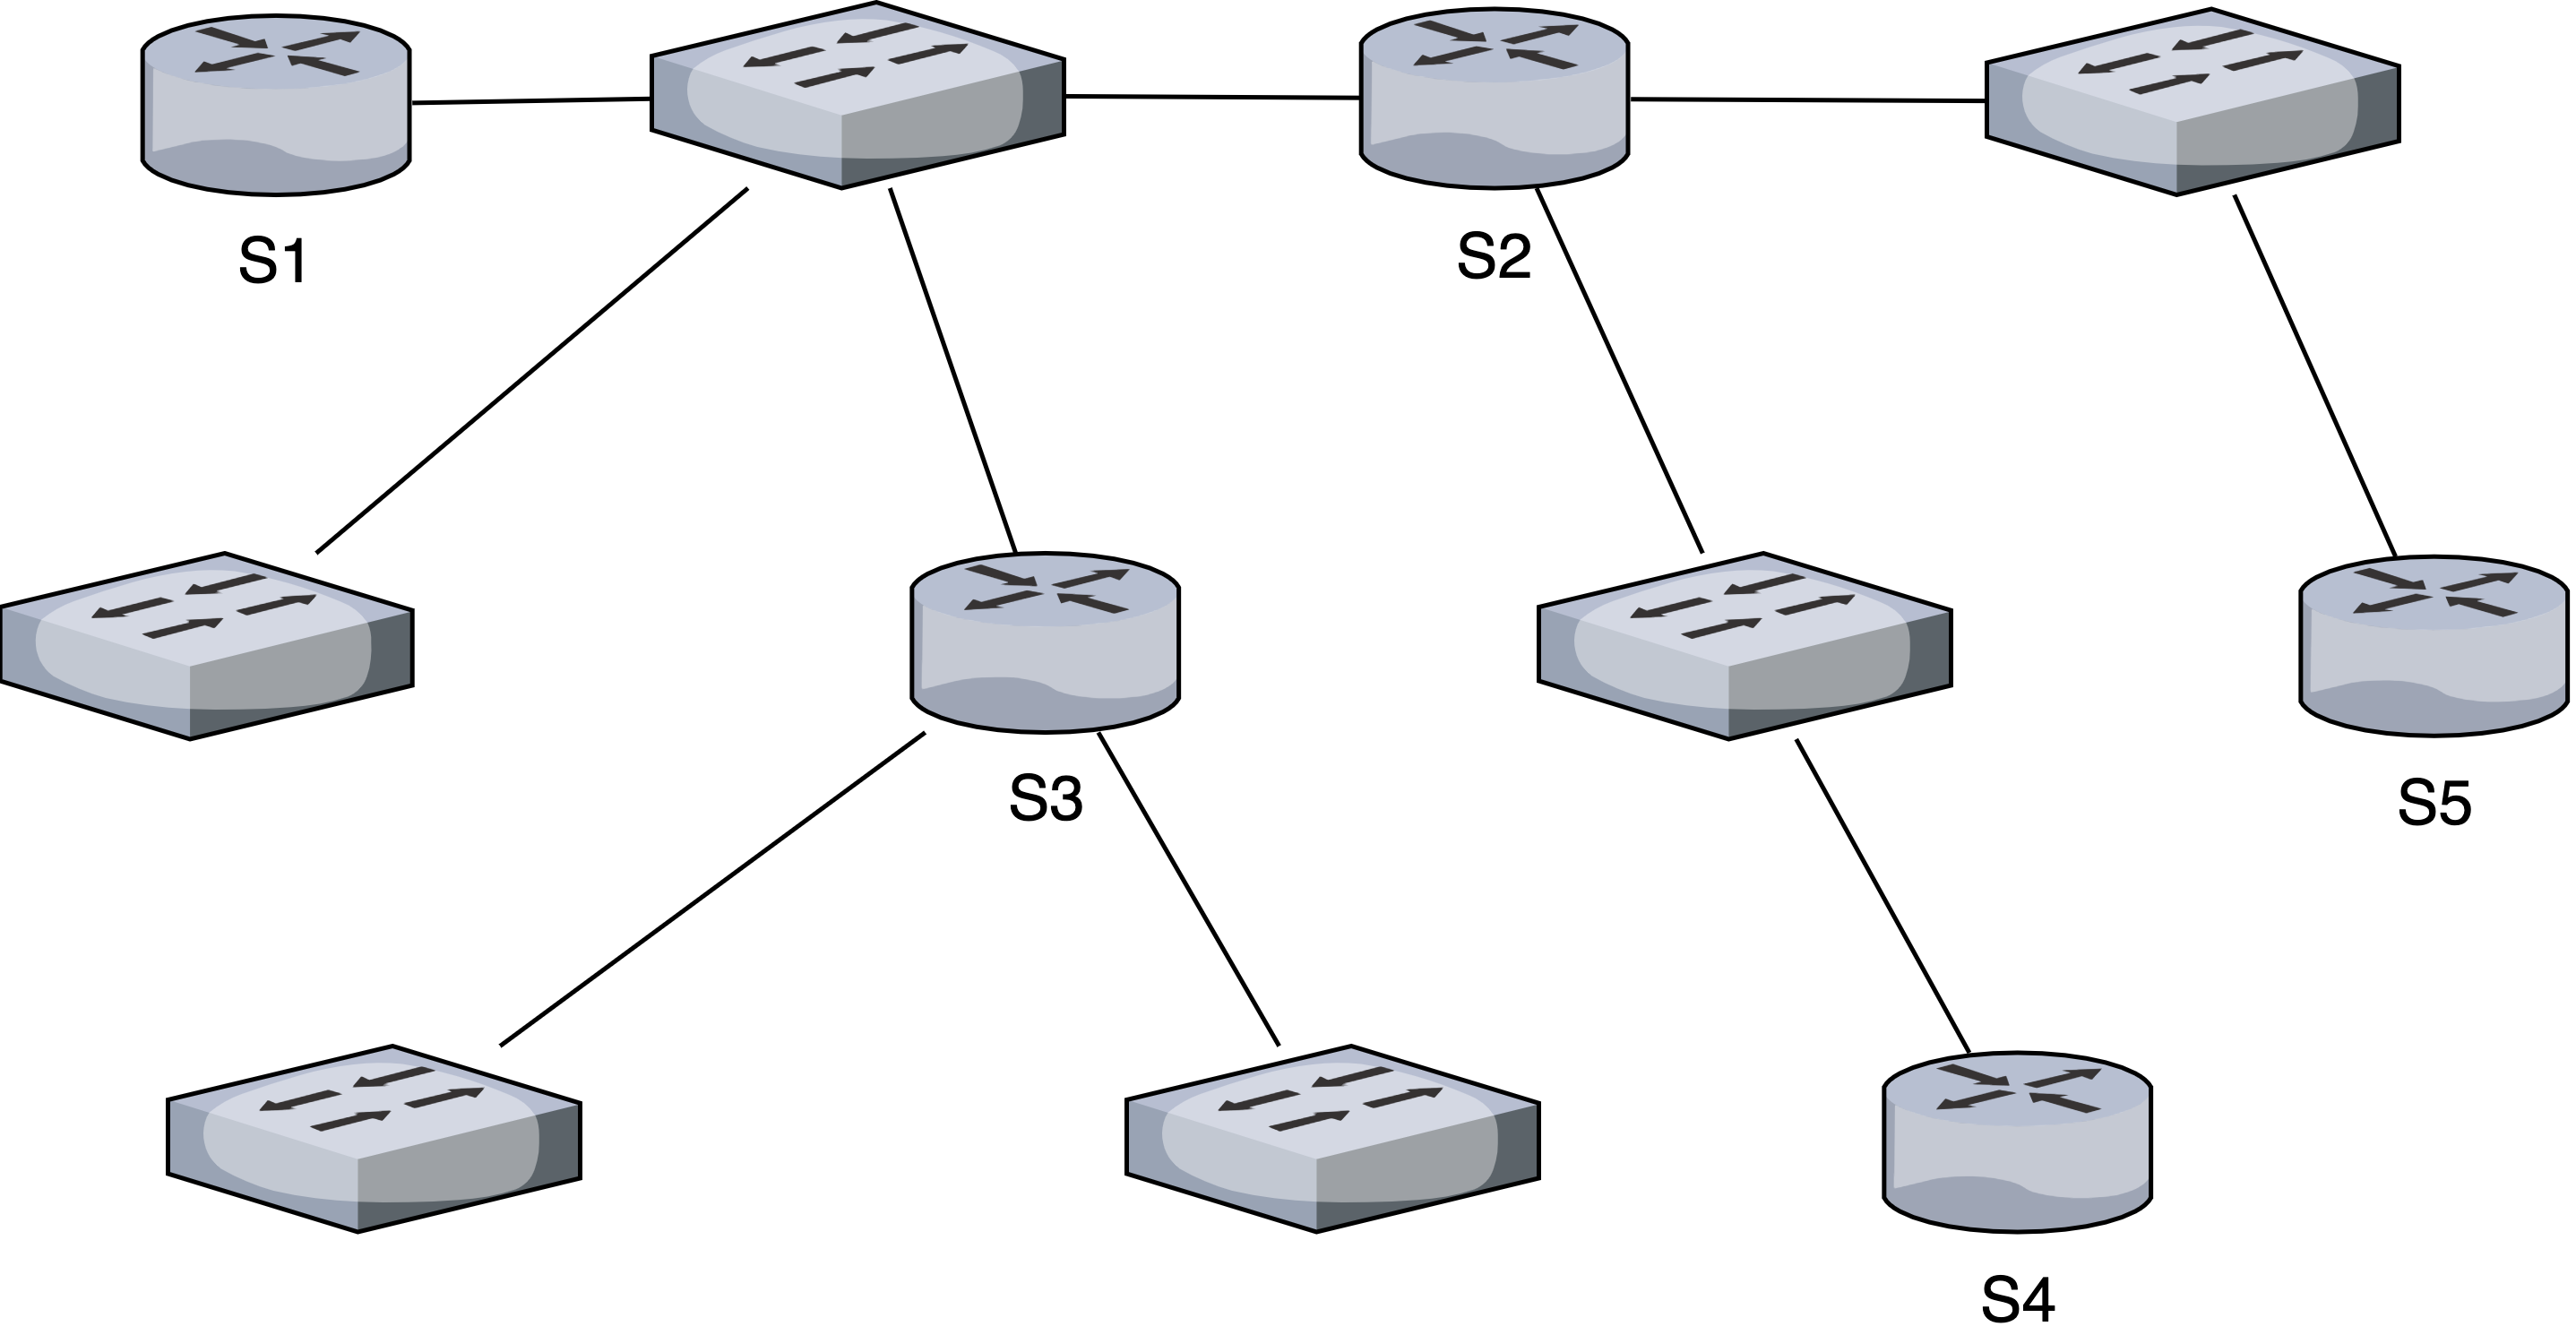
\includegraphics[width=0.8\textwidth]{./figures/ch4-random-topo.png}}
\caption{段路由节点探测列表生成策略拓扑示意图}
\label{fig-ch4-random-topo}
\end{figure}

首先从基于每个节点探测所有其他节点的方案开始展开,如果源段路由节点的报文被发送到另一个段路由节点,那么这个节点会返回一个回复报文来帮助源节点记录时延,由此可以得出一个判断,任何一个节点收到一个探测报文都会认为自己是源节点可达的段路由节点。但是为了降低段路由探测流量的成本,本节不希望源节点探测所有段路由节点,而是探测与自己只有一个段距离的节点。基于这样的目的,所有段路由节点在收到时延探测报文的时候,可以直接返回回复报文并且将该探测报文丢弃。这就使得源段路由节点发出去的探测报文只会被距离自己一个段距离的节点(后文将称为相邻段路由节点)收到,其他距离超过一个段的段路由节点是无法收到该源节点的探测报文的。如图4-4所示,${S_1, S_2, S_3, S_4, S_5}$是具有段路由功能的段路由节点,其他节点为普通交换机,对于$S_1$来说,它发出的探测报文可以到达$S_2$和$S_3$,而发给$S_4$和$S_5$的报文会被$S_2$丢弃;对于$S_2$来说,$S_1, S_3, S_4, S_5$都可以被探测到而不会经过其他段路由节点造成丢包。

基于以上的讨论,本节将段路由节点的探测列表生成流程算法表达如下:

第一步:段路由节点$S_1$在上线的时候从控制器配置文件中获得整个网络中的全部段路由节点列表$S_{all}$;

第二步:段路由节点$S_1$对$S_{all}$中的全部节点发送探测报文;

第三步:记录回复报文的节点列表$S_{neighbor}$,将这些节点作为未来探测列表的成员。

如果有拓扑更新的事件,就会由控制器来触发更新节点的$S_{all}$列表,一旦$S_{all}$列表被更新就需要由该段路由节点对全部节点进行重新探测,进而更新本节点的$S_{neighbor}$。

上述的探测策略是一种确定性方法,可以为每个节点对找到一段之内的全部段路由节点。另外本节还需要提出的一个约束就是需要确保任何一个段路由节点都可以接受到其他任何节点的探测结果,这种探测结果可以是本节点自己探测的结果也可以是获取到其他相邻段路由节点通告的探测结果。虽然举例中是需要对每一个节点$S_i$保留和$S_{neighbor}$之间探测结果,但是实际上在去中心化的分布式算法中,无论接收探测结果的节点还是$S_i$或$S_j$实际上都是等价的,这意味着在考虑$S_i$或$S_j$的情况下指定接收节点的接收策略,实际上是可以将这个策略扩展到全部分布式节点的。有一种方案就是可以让一个中心节点来接收所有的探测结果,但是类似用一个全局控制的控制器节点,它很有可能会遇到性能瓶颈和单点故障,并且在网络扩展的情况下,不过需要扩大控制器的数量,还需要类似控制器东西向控制协议来保证控制节点中数据的一致性,这与本章基于分布式研究算法为了去中心化和提高可扩展性的初衷不符。因此在本章需要找到一种分布式的方法可以为每组段路由节点对找到公共集合节点。即对于每个节点$S_i$来说,都会被$S_{neighbor}$中的节点探测到,这正好与$S_i$的探测列表相同,这就保证了网络中链路的双向时延都会被采集到。

段路由节点收到相邻段路由节点返回报文的时延记录后,会在存储空间中开辟一块内存用作记录4.3.2提到的差分时延矩阵,并将相邻路由节点的时延信息填写在其中,初步构建出时延矩阵。

\begin{figure}[htbp]
\setlength{\abovecaptionskip}{15pt plus 3pt minus 2pt}
\centerline{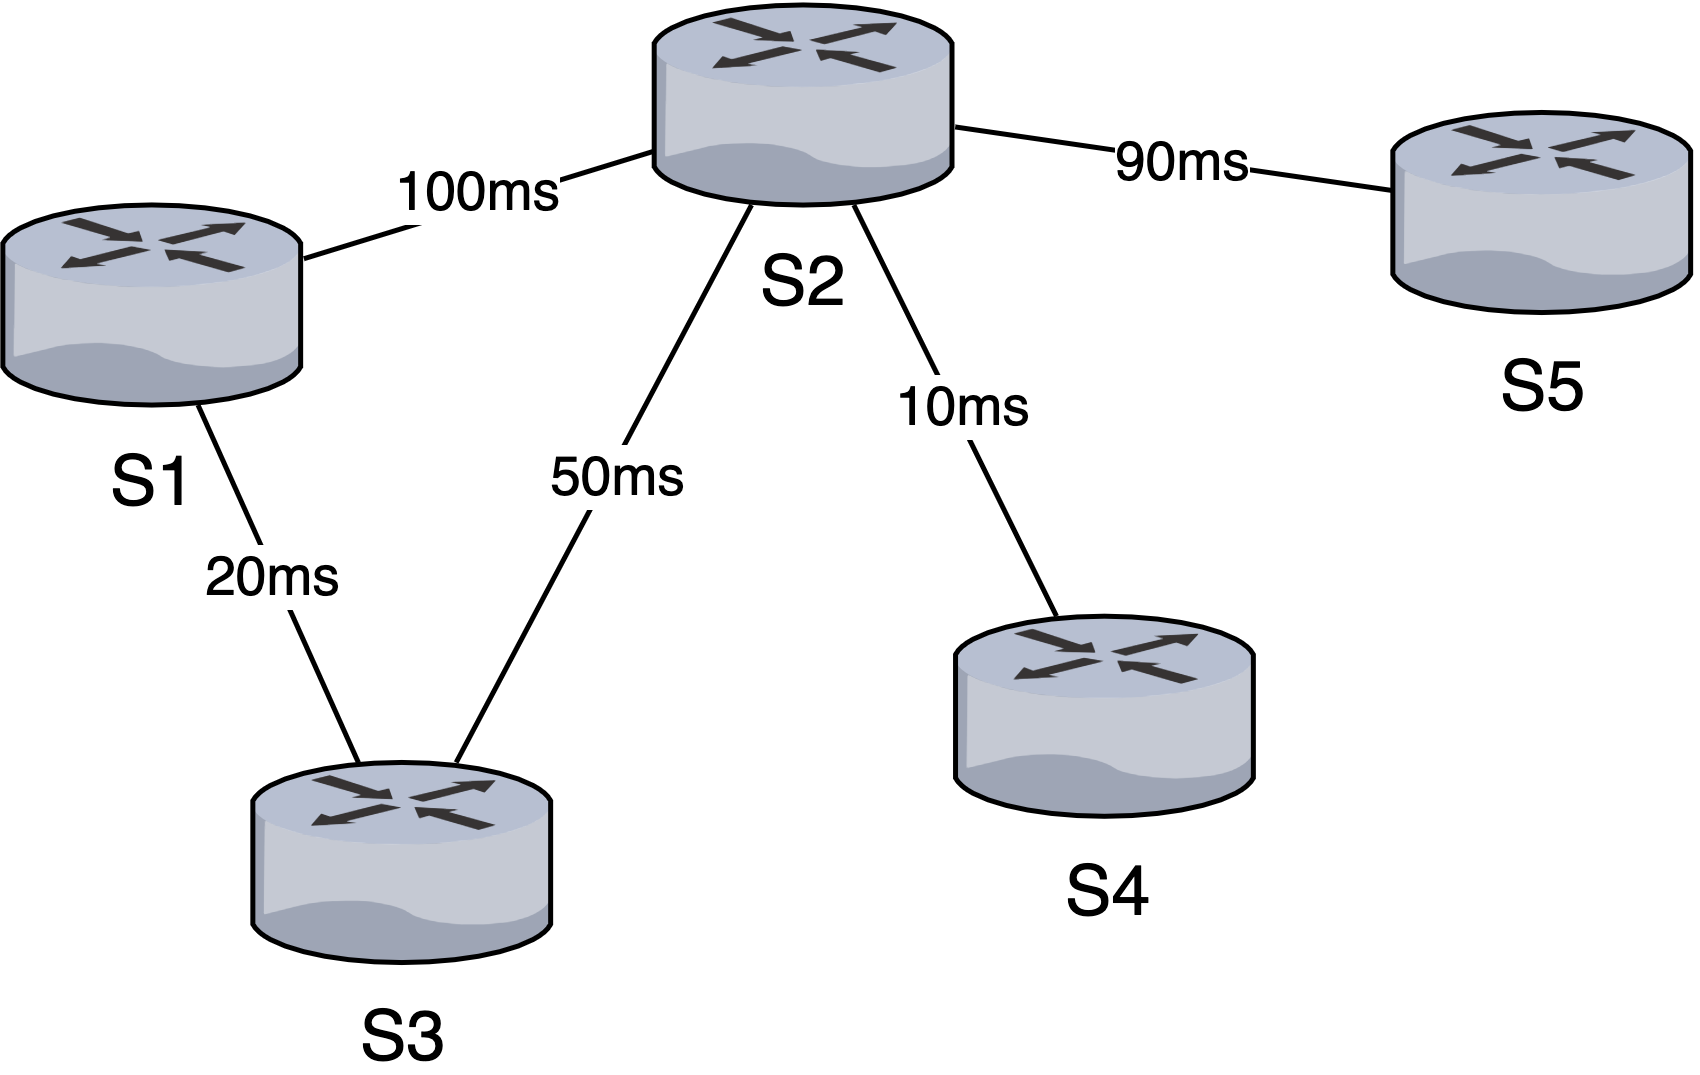
\includegraphics[width=0.6\textwidth]{./figures/ch4-simple-topo.png}}
\caption{简化后段路由节点相邻属性示意图}
\label{fig-ch4-simple-topo}
\end{figure}

\subsection{时延矩阵更新算法}

时延矩阵生成后,最重要的步骤是对时延矩阵进行更新,更新源数据的来源是本段路由节点对外部采集的时延结果和其他段路由节点组播通告结果。结果以键值对的方式存储,索引键为目的节点,值是探测节点到该目的节点的时延。

例如在图中,$S_1$主动探测可以获得$S_2$和$S_3$的时延信息,$S_2$可以获得$S_1, S_3, S_4, S_5$的时延信息,如下表所示:

\begin{table}[htbp]
\begin{tabular}{|p{0.2\textwidth}|p{0.7\textwidth}|}
\hline
1毫秒到10毫秒 & {[}{]} \\ \hline
10毫秒到100毫秒 & {[}S3:\{nil, 20ms\}{]} \\ \hline
100毫秒到1秒 & {[}S2:\{nil, 100ms\}{]} \\ \hline
\end{tabular}
\caption{S1主动探测获得的时延矩阵}
\label{table-S1-get}
\end{table}

$S_2$会将这几条时延信息通告给全网:

\begin{table}[htbp]
\begin{tabular}{|p{0.2\textwidth}|p{0.7\textwidth}|}\hline
1毫秒到10毫秒 & {[}{]} \\ \hline
10毫秒到100毫秒 & {[}S3:\{nil, 50ms\}, S4:\{nil, 10ms\}, S5:\{nil, 90ms\}{]} \\ \hline
100毫秒到1秒 & {[}S1:\{nil, 100ms\}{]} \\ \hline
\end{tabular}
\caption{S2通告的时延矩阵}
\label{table-S2-adverse}
\end{table}

$S_1$接收到这些信息后会将其更新在自己的时延矩阵中:

\begin{table}[htbp]
\begin{tabular}{|p{0.2\textwidth}|p{0.7\textwidth}|}\hline
1毫秒到10毫秒 & {[}{]} \\ \hline
10毫秒到100毫秒 & {[}S3:\{nil, 20ms\}{]} \\ \hline
100毫秒到1秒 & {[}S2:\{nil, 100ms\}, S4:\{S2, 110ms\}, S5:\{S2, 190ms\}{]} \\ \hline
\end{tabular}
\caption{S1接收S2公告后的时延矩阵}
\label{table-S1-after-S2}
\end{table}

在每组新的数据收到后,将执行时延矩阵更新算法,具体算法如下:

对每组数据进行可达性判断并加上沿途的时延,例如$S_1$收到$S_2$到$S_4$的时延是10毫秒时,检查自己没有$S_1$到$S_4$的时延记录,就讲$S_1$到$S_2$的时延和$S_2$到$S_4$的时延加在一起作为$S_1$到$S_4$的时延,并更新到100毫秒到1秒的时延矩阵中。需要注意的是如果本节点本身就对另一个节点可达,那么需要比较原本的方案和新生成的方案的时延,在时延矩阵中保留时延较短的方案。这样使得整个时延矩阵只会保留较小的时延方案,并不是所有的时延方案。

本节点将迭代相加直到更新本段路由节点到其他所有可达节点的时延,如果时延有降低则需要在算法的差分数据结构中进行遍历并对可以降级的时延和对应下一跳节点进行更新;如果时延有增高则需要在算法的差分数据结构中进行遍历并对需要升级的时延和对应的下一跳节点进行更新。当所有更新结束之后,就将新的时延矩阵组播或者广播通告出去。

\begin{figure}[htbp]
\setlength{\abovecaptionskip}{15pt plus 3pt minus 2pt}
\centerline{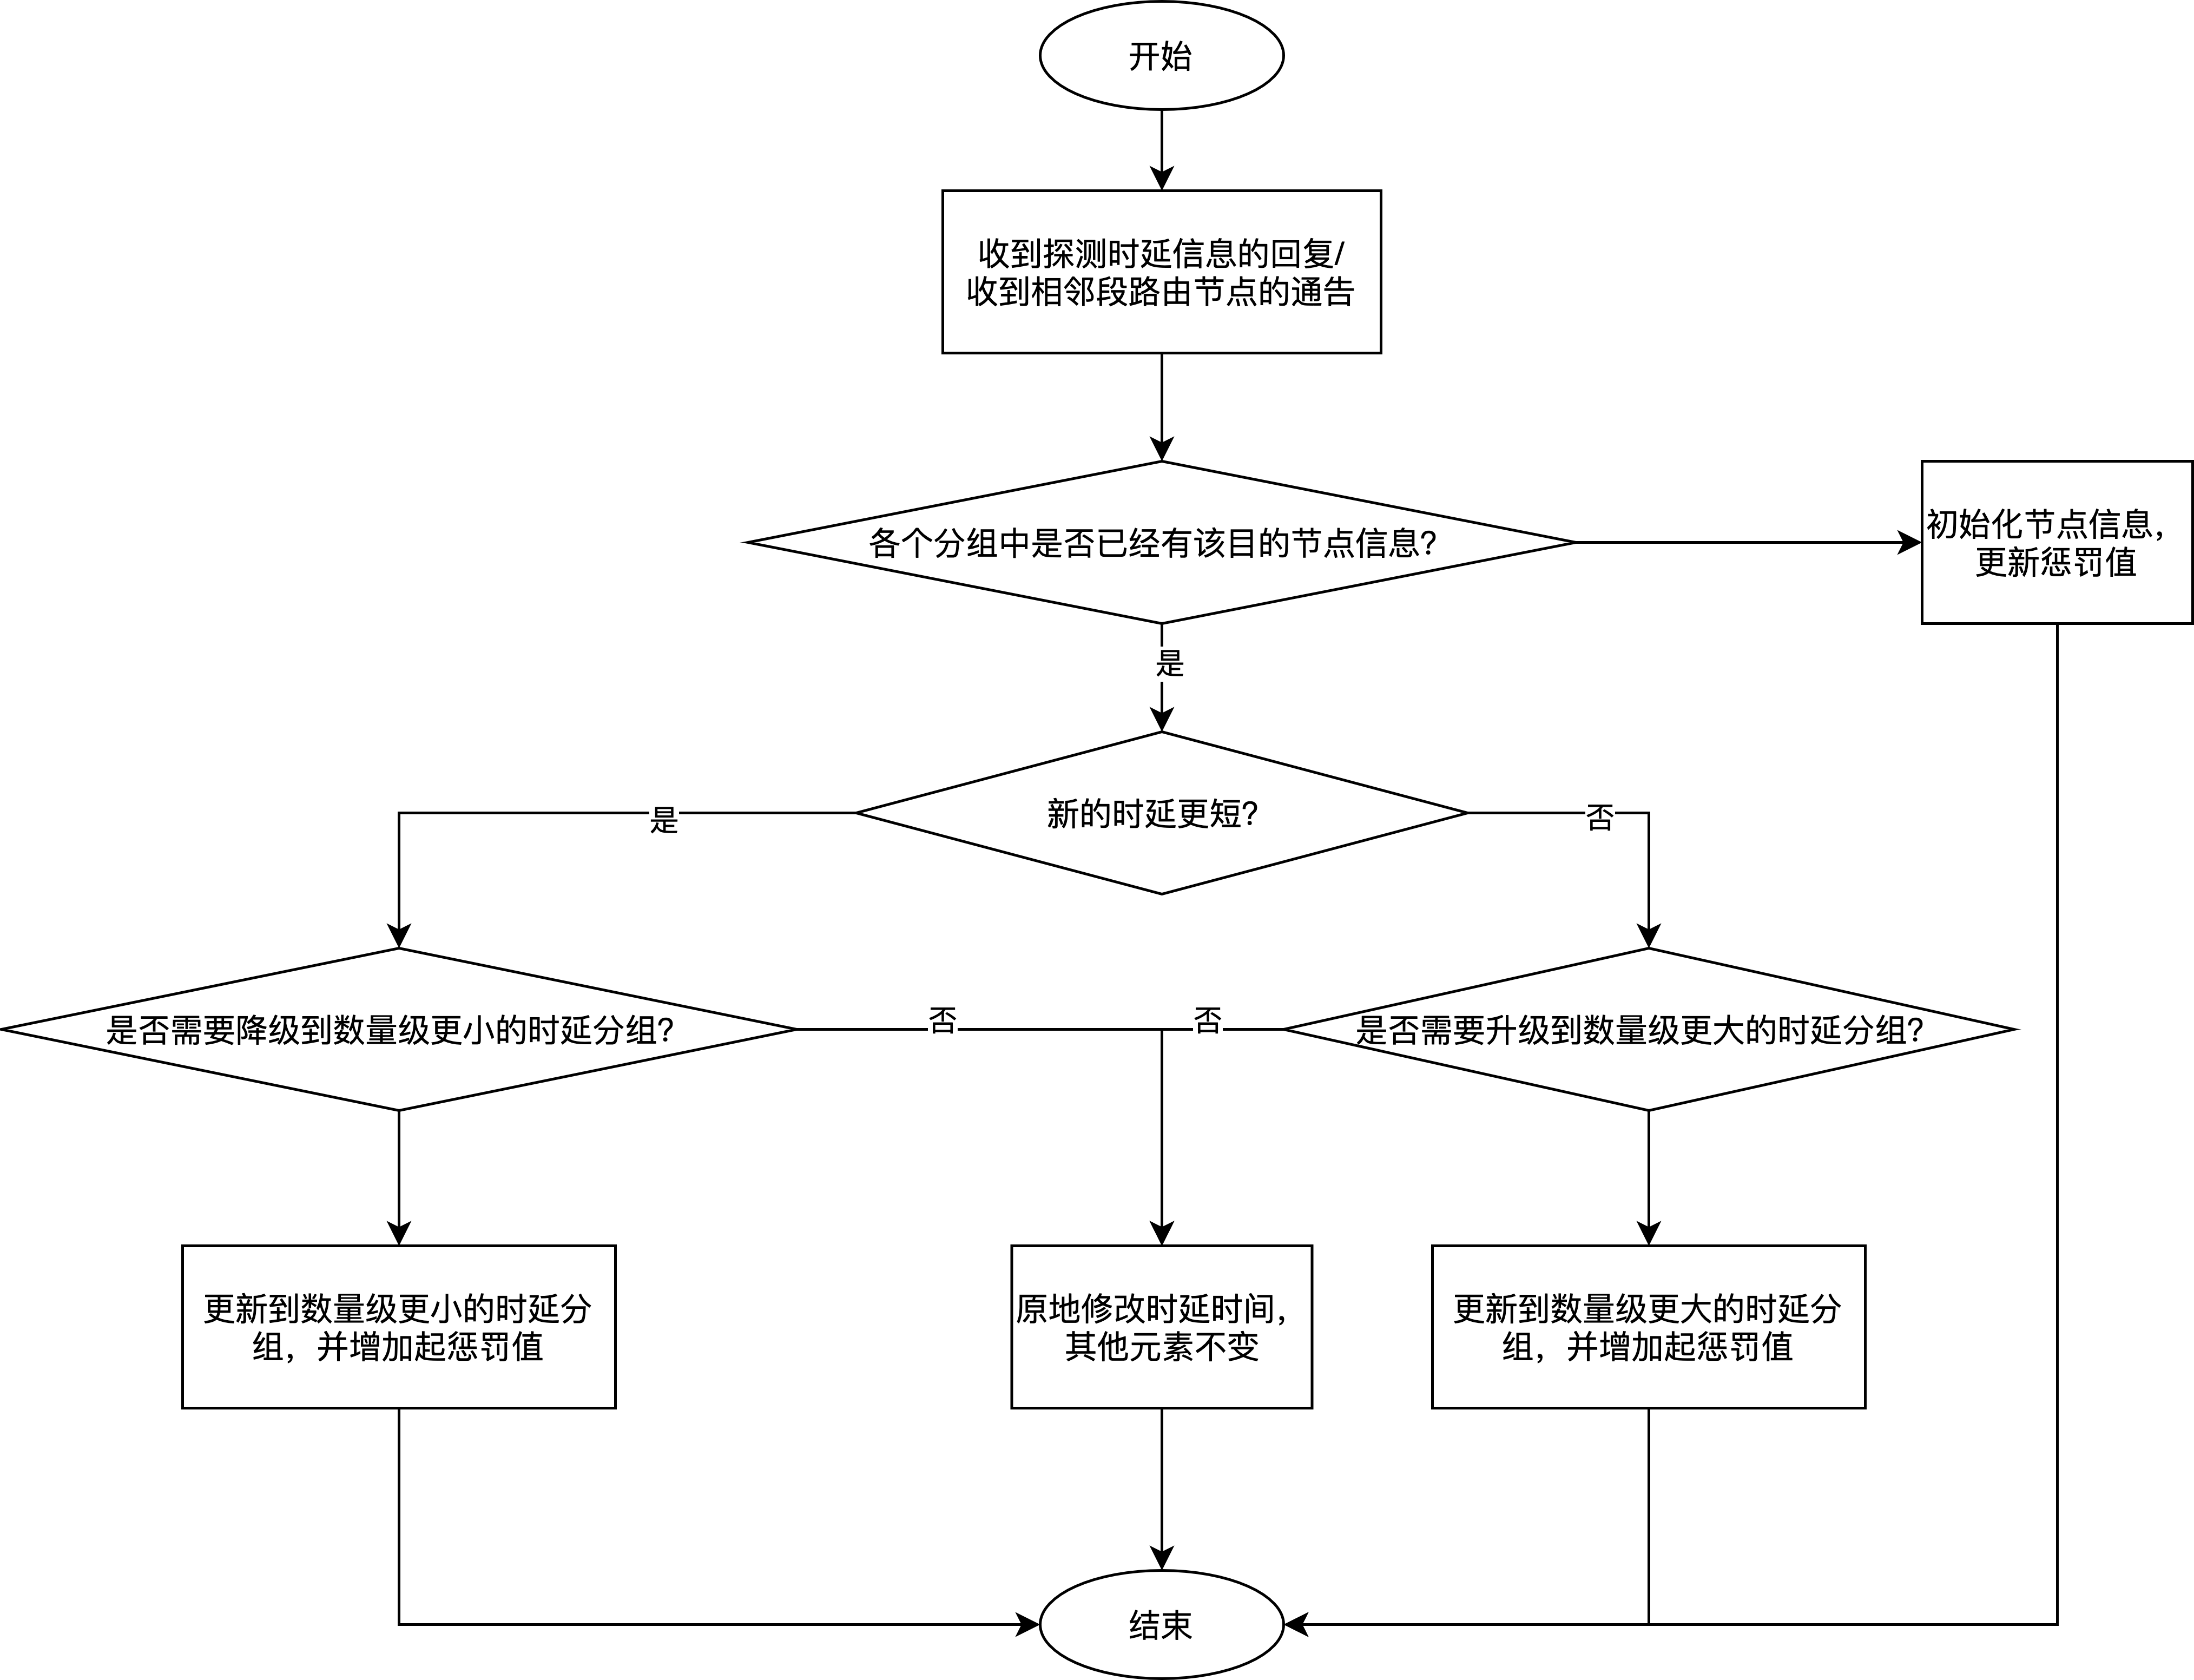
\includegraphics[width=1\textwidth]{./figures/ch4-sr-update.png}}
\caption{时延矩阵更新算法示意图}
\label{fig-ch4-sr-update}
\end{figure}

在使用段路有的较大规模网络中,由于段路由节点数目增多,段路由时延矩阵可能会变得变得十分庞大,这不光会使得存储时延矩阵将会占有大量的交换机内存资源,而且还会使得传输和处理段路由节点探测的时延信息所必需的带宽以及处理这些时延信息都需要大量的资源。因此考虑使用类似路由聚合(Routes Aggregation)的方式再时延矩阵更新算法中使用段路由节点聚合来减小段路由时延矩阵的规模,这是由于段路有节点其实是具有一定聚合的特性的,在第三章中使用的节点组中心度就是一个体现。另外通过对段路由节点的目的条目进行聚合,也可以隐藏一些过于详细的段路由节点时延信息,从而减少选路结果震荡对段路由网络带来的影响。

关于时延矩阵的更新有一个需要关注的挑战点,就是如何防止选路结果来回震荡。这是因为当一组段路由节点被选中的时候,这一组对应的时延就会增高,如果这个时候采集到了数据就很有可能对这个段路由节点的时延进行降级,而一旦这股流量结束了,采集到的时延就会降低,这个时候这个节点所属的差分时延组就会升级,而这样的变动可以看作是一种不稳定的体现,它这种在某组时延路由表中反复出现和消失就像是路由不稳定时表现出来的路由震荡,在网络中发生路由振荡时,路由器就会向邻居发布路由更新,收到路由更新报文的路由器需要重新计算路由并修改路由表。所以频繁的路由振荡会消耗大量的带宽资源和路由器CPU资源,严重时会影响到网络的正常工作。面对这样的情况,边界网关协议中有一个解决路由不稳定的思路,即路由衰减(Route Dampening)。多数情况下,边界网关协议都应用于复杂的网络环境中,路由变化十分频繁。为了防止持续的路由振荡带来的不利影响,边界网关协议使用路由衰减来抑制不稳定的路由。边界网关协议中使用惩罚值(Penalty Value)来衡量一条路由的稳定性,惩罚值的计算是当路由每发生一次振荡,边界网关协议便会给此路由增加一定的惩罚值(一般的做法是路由从激活状态变为未激活状态,惩罚值需要增加1000,路由在激活状态,收到新的路由更新,惩罚值加500),惩罚值越高就说明路由越不稳定。当惩罚值超过抑制阈值(Suppress Value)时,此路由被抑制,不加入到路由表中,也不再向其他边界网关协议对等体发布路由更新报文。而被抑制的路由每经过一段时间,惩罚值便会减少一半,这个时间称为半衰期(Half-life)。当惩罚值降到再使用阈值(Reuse Value)时,此路由变为可用并被加入到路由表中,同时向其他边界网关协议对等体发布路由更新报文。

参考边界网关协议的路由衰减机制,本章设计了对时延矩阵进行震荡抑制的方案,即有节点从不可达被加入时延矩阵时,惩罚值需要增加1000;每次有节点需要被升级或者降级的时候,就会给其惩罚值加500。并同样为其设置一个半衰期使得这个惩罚值可以随稳定时间增长而逐渐降低,本算法中的半衰期设置为往返时延与计算路由收敛时长和的两倍,实验中取1秒。与此同时当惩罚值到达800的抑制阈值时不可使用该段路由方案,直到降到200的重用阈值时可以开始使用,整个惩罚值随时间长度增长的变化趋势如图4-7所示,第2秒时新的段路由方案加入因此该方案当前惩罚值是1000,1秒的半衰期后降为500,第5秒和第7秒分别产生了该段路由方案在时延分组中的迁移,因此都增加了500的惩罚值,之后该段路由方案稳定,在第10秒的时候降低到重用阈值200以下开始可以被使用。

\begin{figure}[htbp]
\setlength{\abovecaptionskip}{15pt plus 3pt minus 2pt}
\centerline{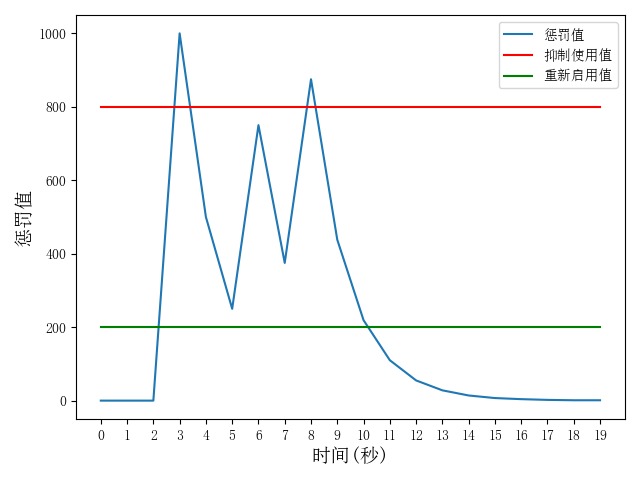
\includegraphics[width=0.8\textwidth]{./figures/ch4-penalty-value.png}}
\caption{惩罚值和半衰期随时间变化示意图}
\label{fig-ch4-penalty-value}
\end{figure}

而对于需要选择段路由航点列表方案的算法来说,在段路由节点列表的选择上则需要参考惩罚值,相同差分区域内进行段路由节点列表的选择时,会更倾向于选择惩罚值更低的段路由节点。

\subsection{段路由航点列表生成算法}

每个段路由节点将探测到的时延信息通告出去,并且所有节点的时延矩阵都趋近于收敛的时候,可以开始对服务流量开始执行选路算法。为简化问题,假设服务流量的源地址和目的地址都是段路由节点,这种假设实际上和真实网络中的情况有所出入,实际网络中源地址和目的地址一定都是主机的地址,但由于网络中的路由是按照网段进行最长前缀匹配路由的,所以可以按照交换机节点的位置选择流量调度的终点。因此段路由航点列表生成算法问题可以简化表达为对于一对段路由节点$S_i$和$S_j$,如何选择符合时延需求的段路由航点标签列表。

当带有时延请求的报文到达$S_i$时,$S_i$将在对应的差分段$[D_n^{start},D_n^{end}]$内寻找可行的方案,$D_n^{start}{<D}_{target}<D_n^{end}$,由于差分段内使用优先级队列进行存储,因此可以认为所有时延方案的排列是有序的,因此可以用二分法在$O\left(\sqrt n\right)$的时间内找到符合要求的方案。但是正好符合时延需求的方案大概率是不存在的,这里存在几种情况:第一种$[D_n^{start},D_n^{end}]$存在可行方案但是都比$D_{target}$大,这种情况下可以视网络具体情况而定,如果QPS较大,可以选择同一差分等级中当前时延最小的方案;如果QPS还比较小,也可以选择更短时延分段组内时延最大的方案,这意味着建立因此需要向上兼容选择时延较低的相邻方案,而且如果该业务的优先级很低也可以选择拒绝。第二种$[D_n^{start},D_n^{end}]$存在可行方案但是都比$D_{target}$小,那么直接选择这组内时延组大的方案即可。第三种是$\left[D_n^{start},D_n^{end}\right]$内不存在方案,那么处理方式和第一种一样。第四种就是最符合预期的方案$\left[D_n^{start},D_n^{end}\right]$内存在合适方案,且有比目标时延大的,也有比目标时延小的,此时按照二分法获取符合目标时延需求的方案即可。第五种则是每种分组时延的方案中都没有目的地址是$S_j$的方案,即$S_j$对于$S_i$来说不可达,可以直接拒绝服务请求。流程总结如图4-8所示。

\begin{figure}[htbp]
\setlength{\abovecaptionskip}{15pt plus 3pt minus 2pt}
\centerline{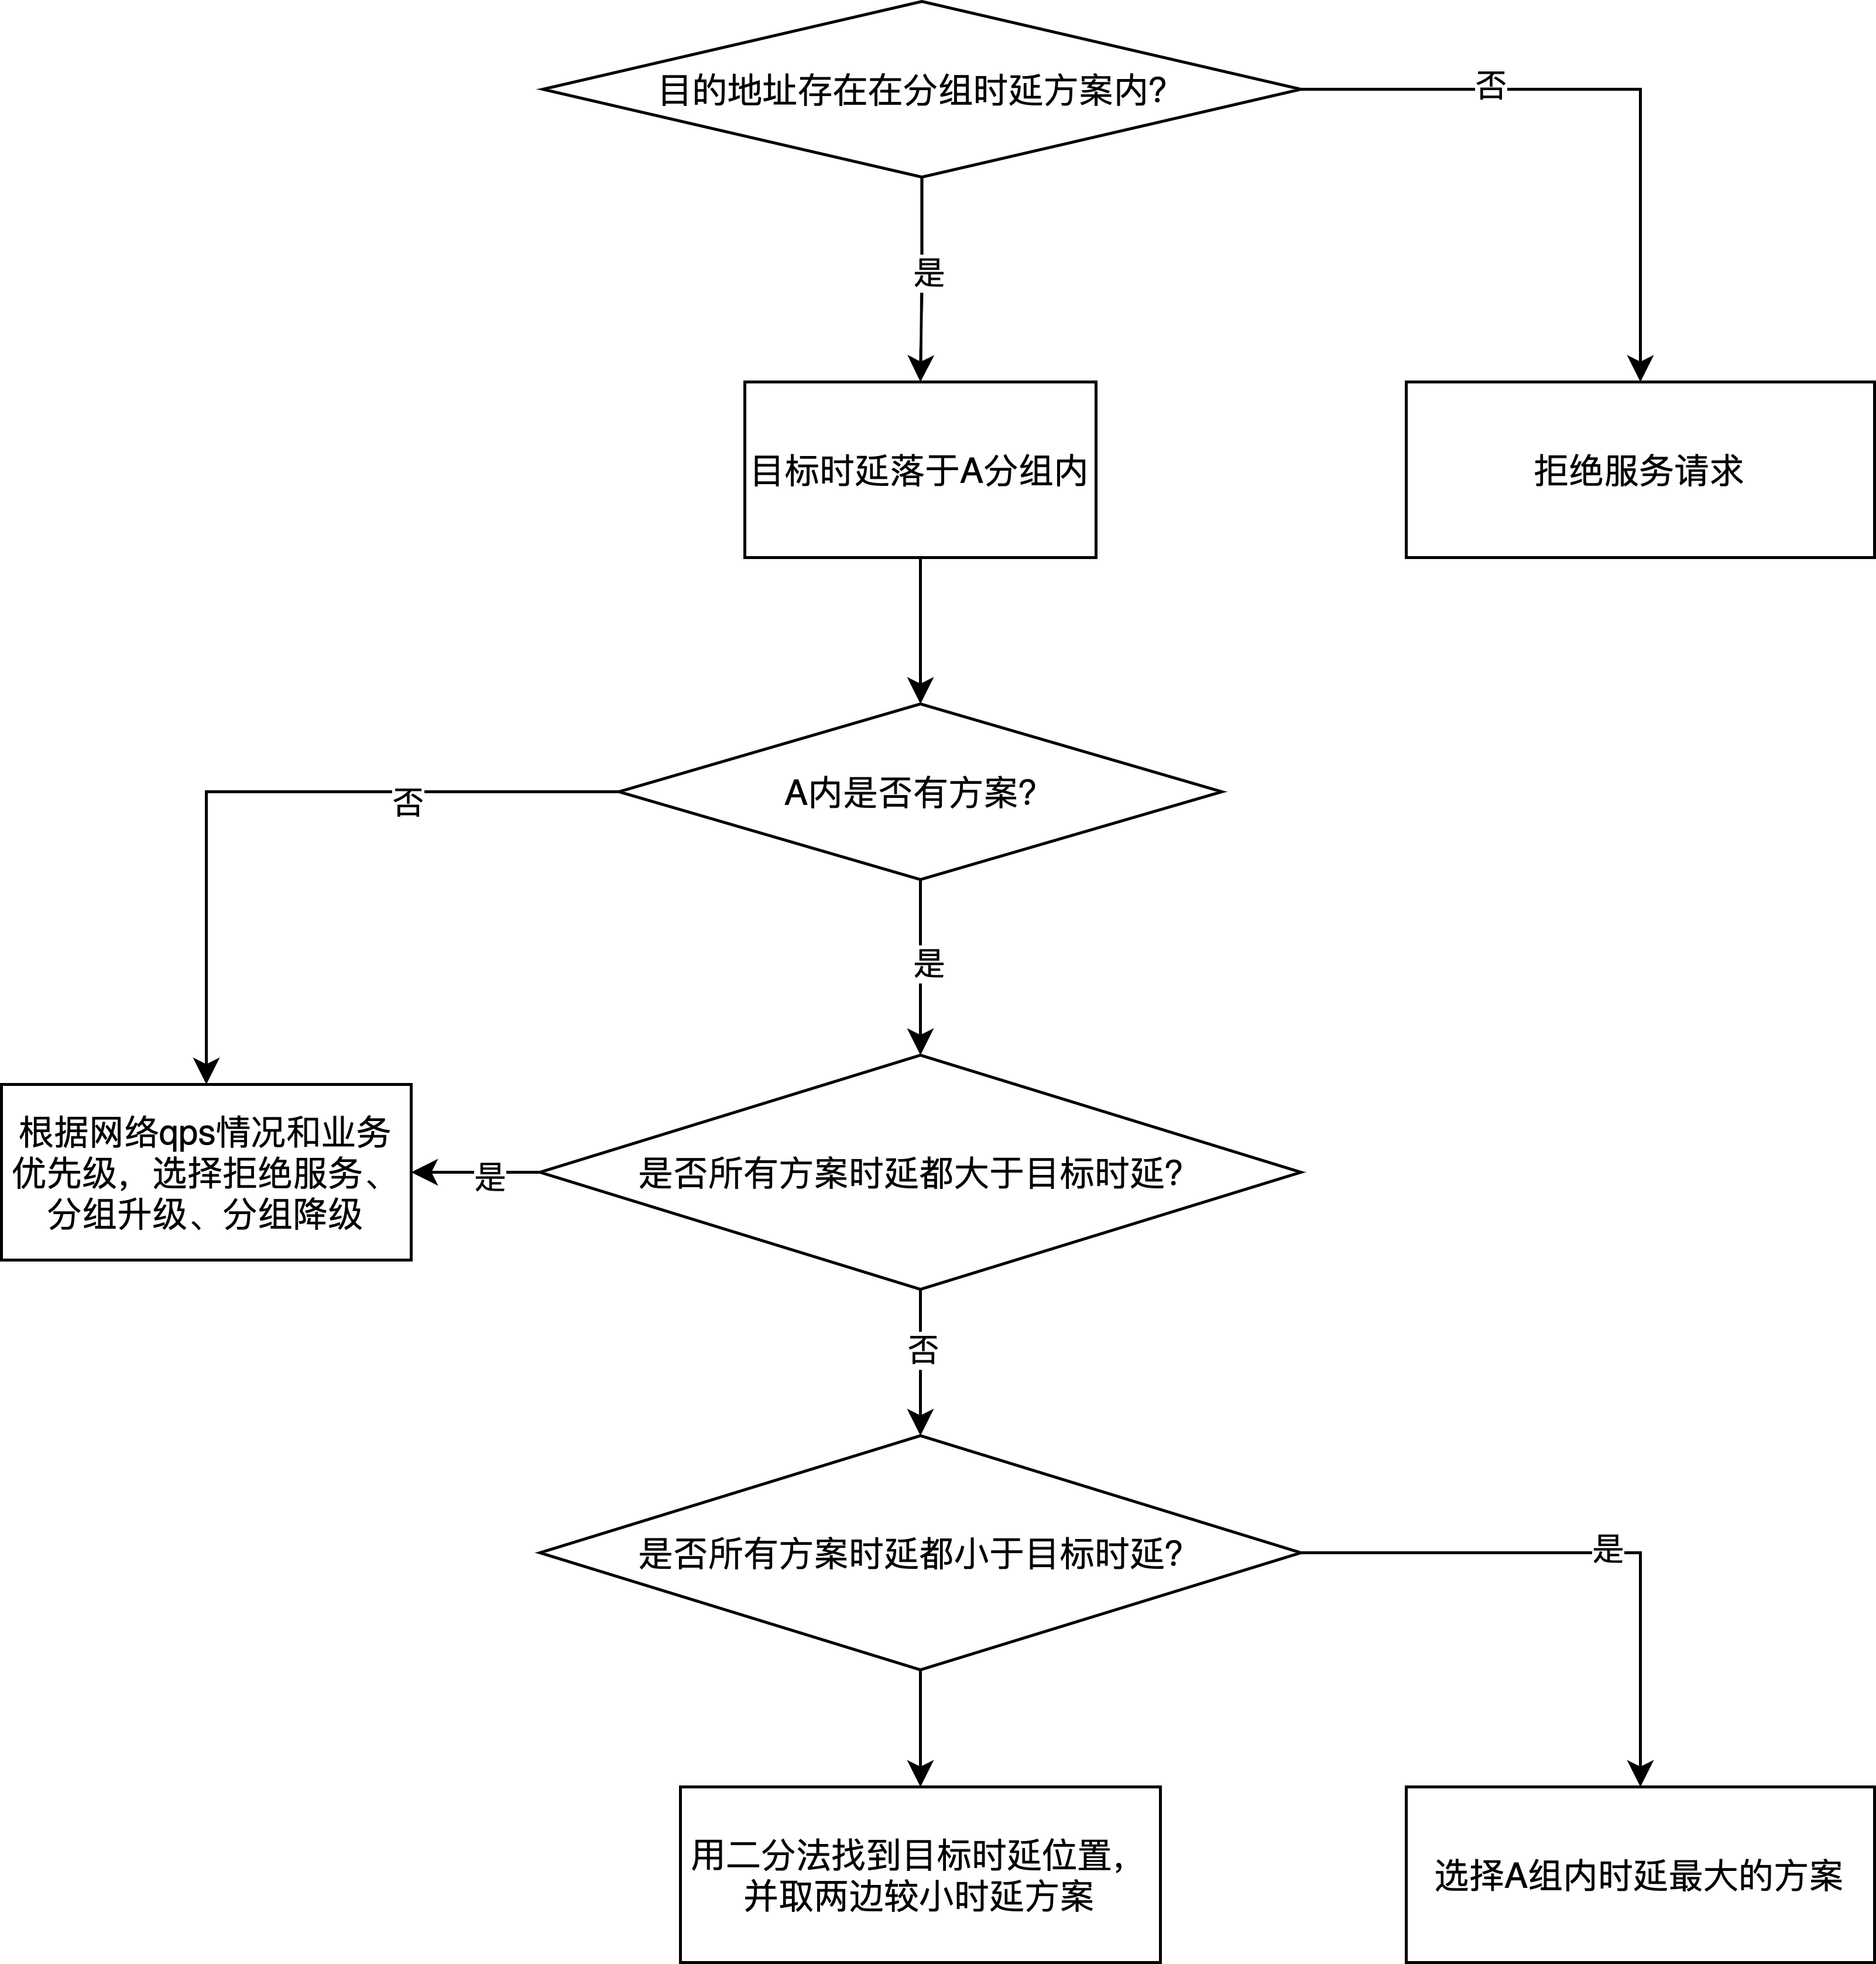
\includegraphics[width=0.9\textwidth]{./figures/ch4-find-sr-ans.png}}
\caption{段路由方案生成算法示意图}
\label{fig-ch4-find-sr-ans}
\end{figure}
    
确定选择的时延的方案后,就需要用递归的方式寻找整个段路由路径,例如$S_1$收到目的地知识$S_4$的报文,并且时延需求是150毫秒,那么在经过复杂化的下表中,首先定位到100毫秒到1秒的分组中,先通过哈希获取$S_4$方案的子列表头端点,最后通过二分法找到符合时延需求的段路由方案。在找到段路由方案之后,通过每组方案第一个元素代表的上一跳信息,逐步用递归的方式找到整个段路由列表。例如在下表中找到$S_4$之后,通过$S_4$的第一个元素$S_2$找到目的地址是$S_2$的方案,发现目的地址为$S_2$时下一跳时空,这说明已经递归完毕,可以返回整个段路由方案$S_1->S_2->S_4$。

\begin{table}[htbp]
\begin{tabular}{|p{0.2\textwidth}|p{0.7\textwidth}|}
\hline
1毫秒到10毫秒 & {[}{]} \\ \hline
10毫秒到100毫秒 & {[}S3:\{nil, 20ms\}{]} \\ \hline
100毫秒到1秒 & {[}S2:\{nil, 100ms\}, S4:\{S2, 110ms\}, S5:\{S2, 190ms\}{]} \\ \hline
\end{tabular}
\caption{S1时延矩阵}
\label{table-S1-delay-metric}
\end{table}

将上述算法总结为算法流程图如图4-9所示:

\begin{figure}[htbp]
\setlength{\abovecaptionskip}{15pt plus 3pt minus 2pt}
\centerline{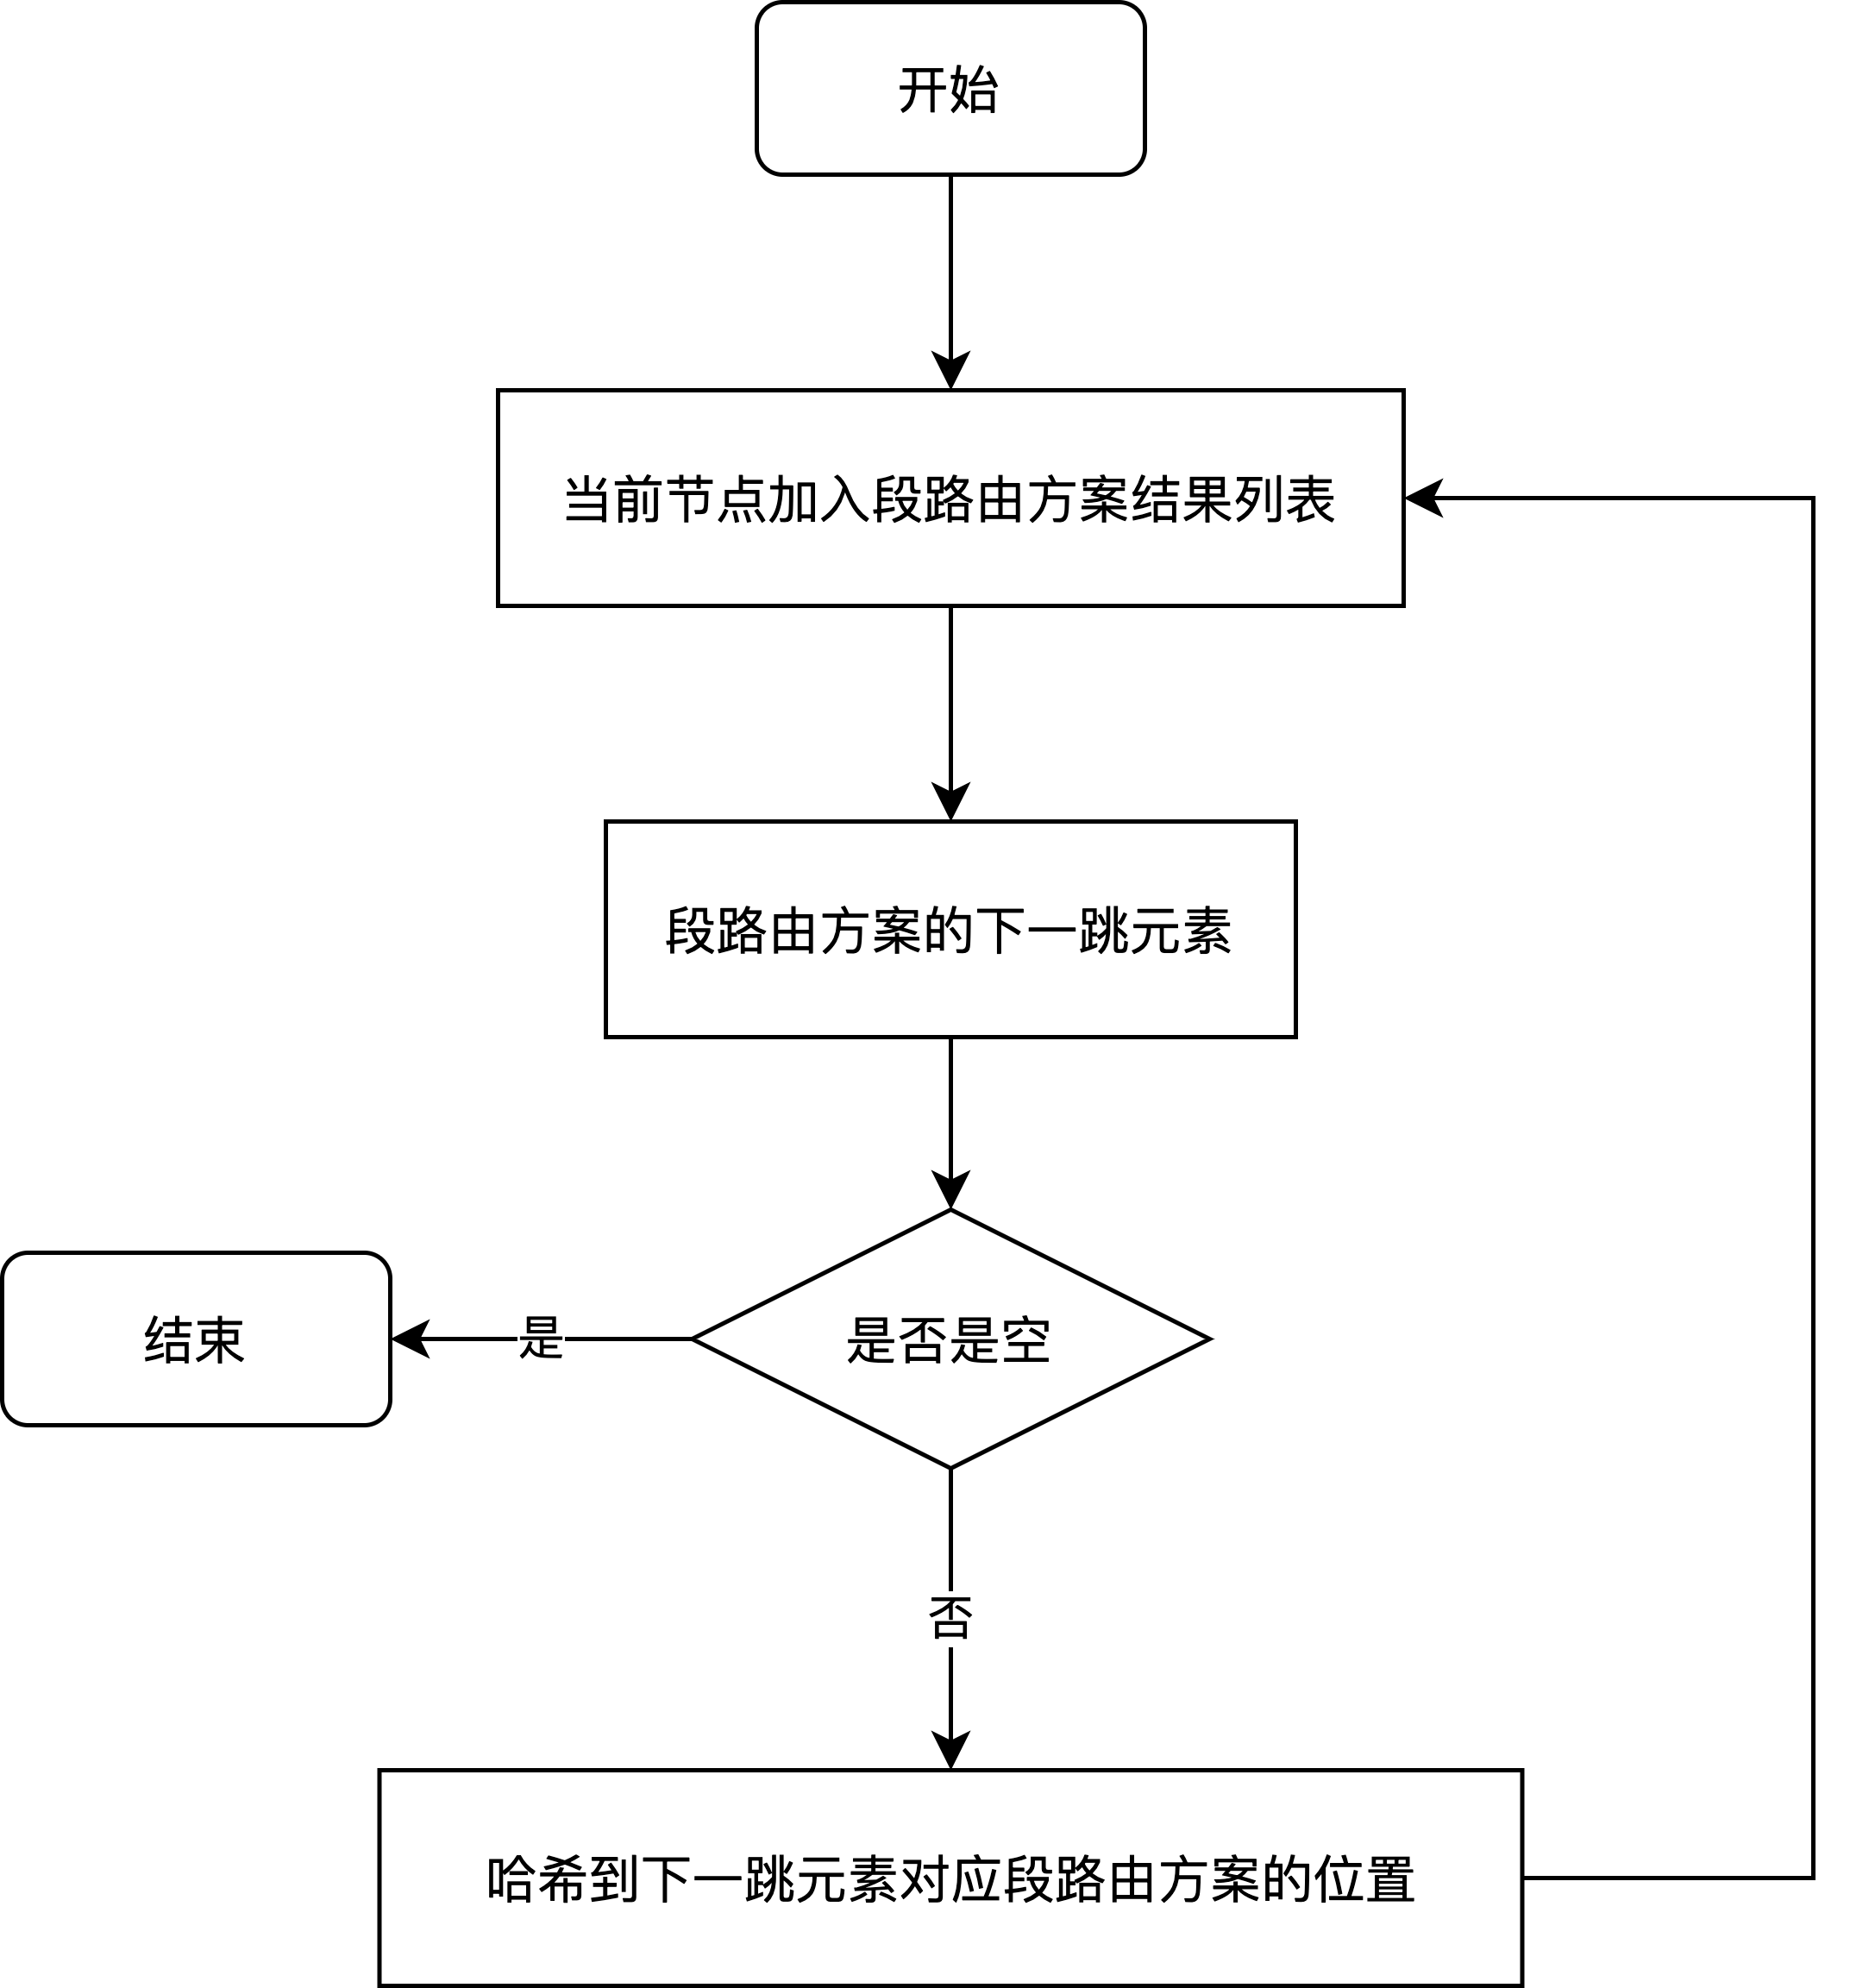
\includegraphics[width=0.8\textwidth]{./figures/ch4-sr-init.png}}
\caption{段路由标签列表生成算法示意图}
\label{fig-ch4-sr-init}
\end{figure}

\subsection{算法时间复杂度分析}

本章提出算法的时延复杂度如下:

时延矩阵更新算法需要遍历所有的方案,最好情况$O\left(1\right)$的时间复杂度,最差情况下具有$O\left(n\right)$的时间复杂度,因此平均时间复杂度为$O\left(n\right)$;段路由航点列表生成算法需要首先找到节点位置,最好情况下$O\left(1\right)$的时间复杂度,最差情况下$O\left(\sqrt n\right)$,平均时间复杂度为$O\left(\sqrt n\right)$;第二步生成整个段列表,只需要递归即可,最好情况下时间复杂度为$O\left(1\right)$,最差情况下需要递归到全部节点即$O\left(n\right)$,平均为$O\left(n\right)$。综上所述由于本章使用较多的哈希数据结构,使得整体时间复杂度较低。

\section{实验验证}

本章的实验是对分布式算法进行验证,因此除了对算法对时延效果的保障外,也会考虑算法的时间空间复杂度和时间复杂度。对比组主要有边界网关协议和开放最短路径优先的分布式协议,比较计算资源占用的情况、时延保障的效果和对网络吞吐量的影响,最终得出本章分布式段路由航点选择算法在时延保障上的有效性。本节将首先介绍实验设置,然后在数值和仿真实验中评估基于差分时延路径选择算法的性能和效果。

\subsection{实验环境}

1. 实验装置

本章提出的分布式段路由航点选择算法在实验验证中由C++实现。段路由节点主进程内有三个主要线程,第一个是用于对探测列表内段路由节点进行时延探测并更新时延矩阵的线程,第二个是接收其他段路由节点通告时延矩阵结论并更新时延矩阵的线程,第三个是对服务流量进行航点列表生成算法的进程。段路由节点的探测目标节点列表由控制器生成,通过管理配置的方式下发给段路由节点。

\begin{figure}[htbp]
\setlength{\abovecaptionskip}{15pt plus 3pt minus 2pt}
\centerline{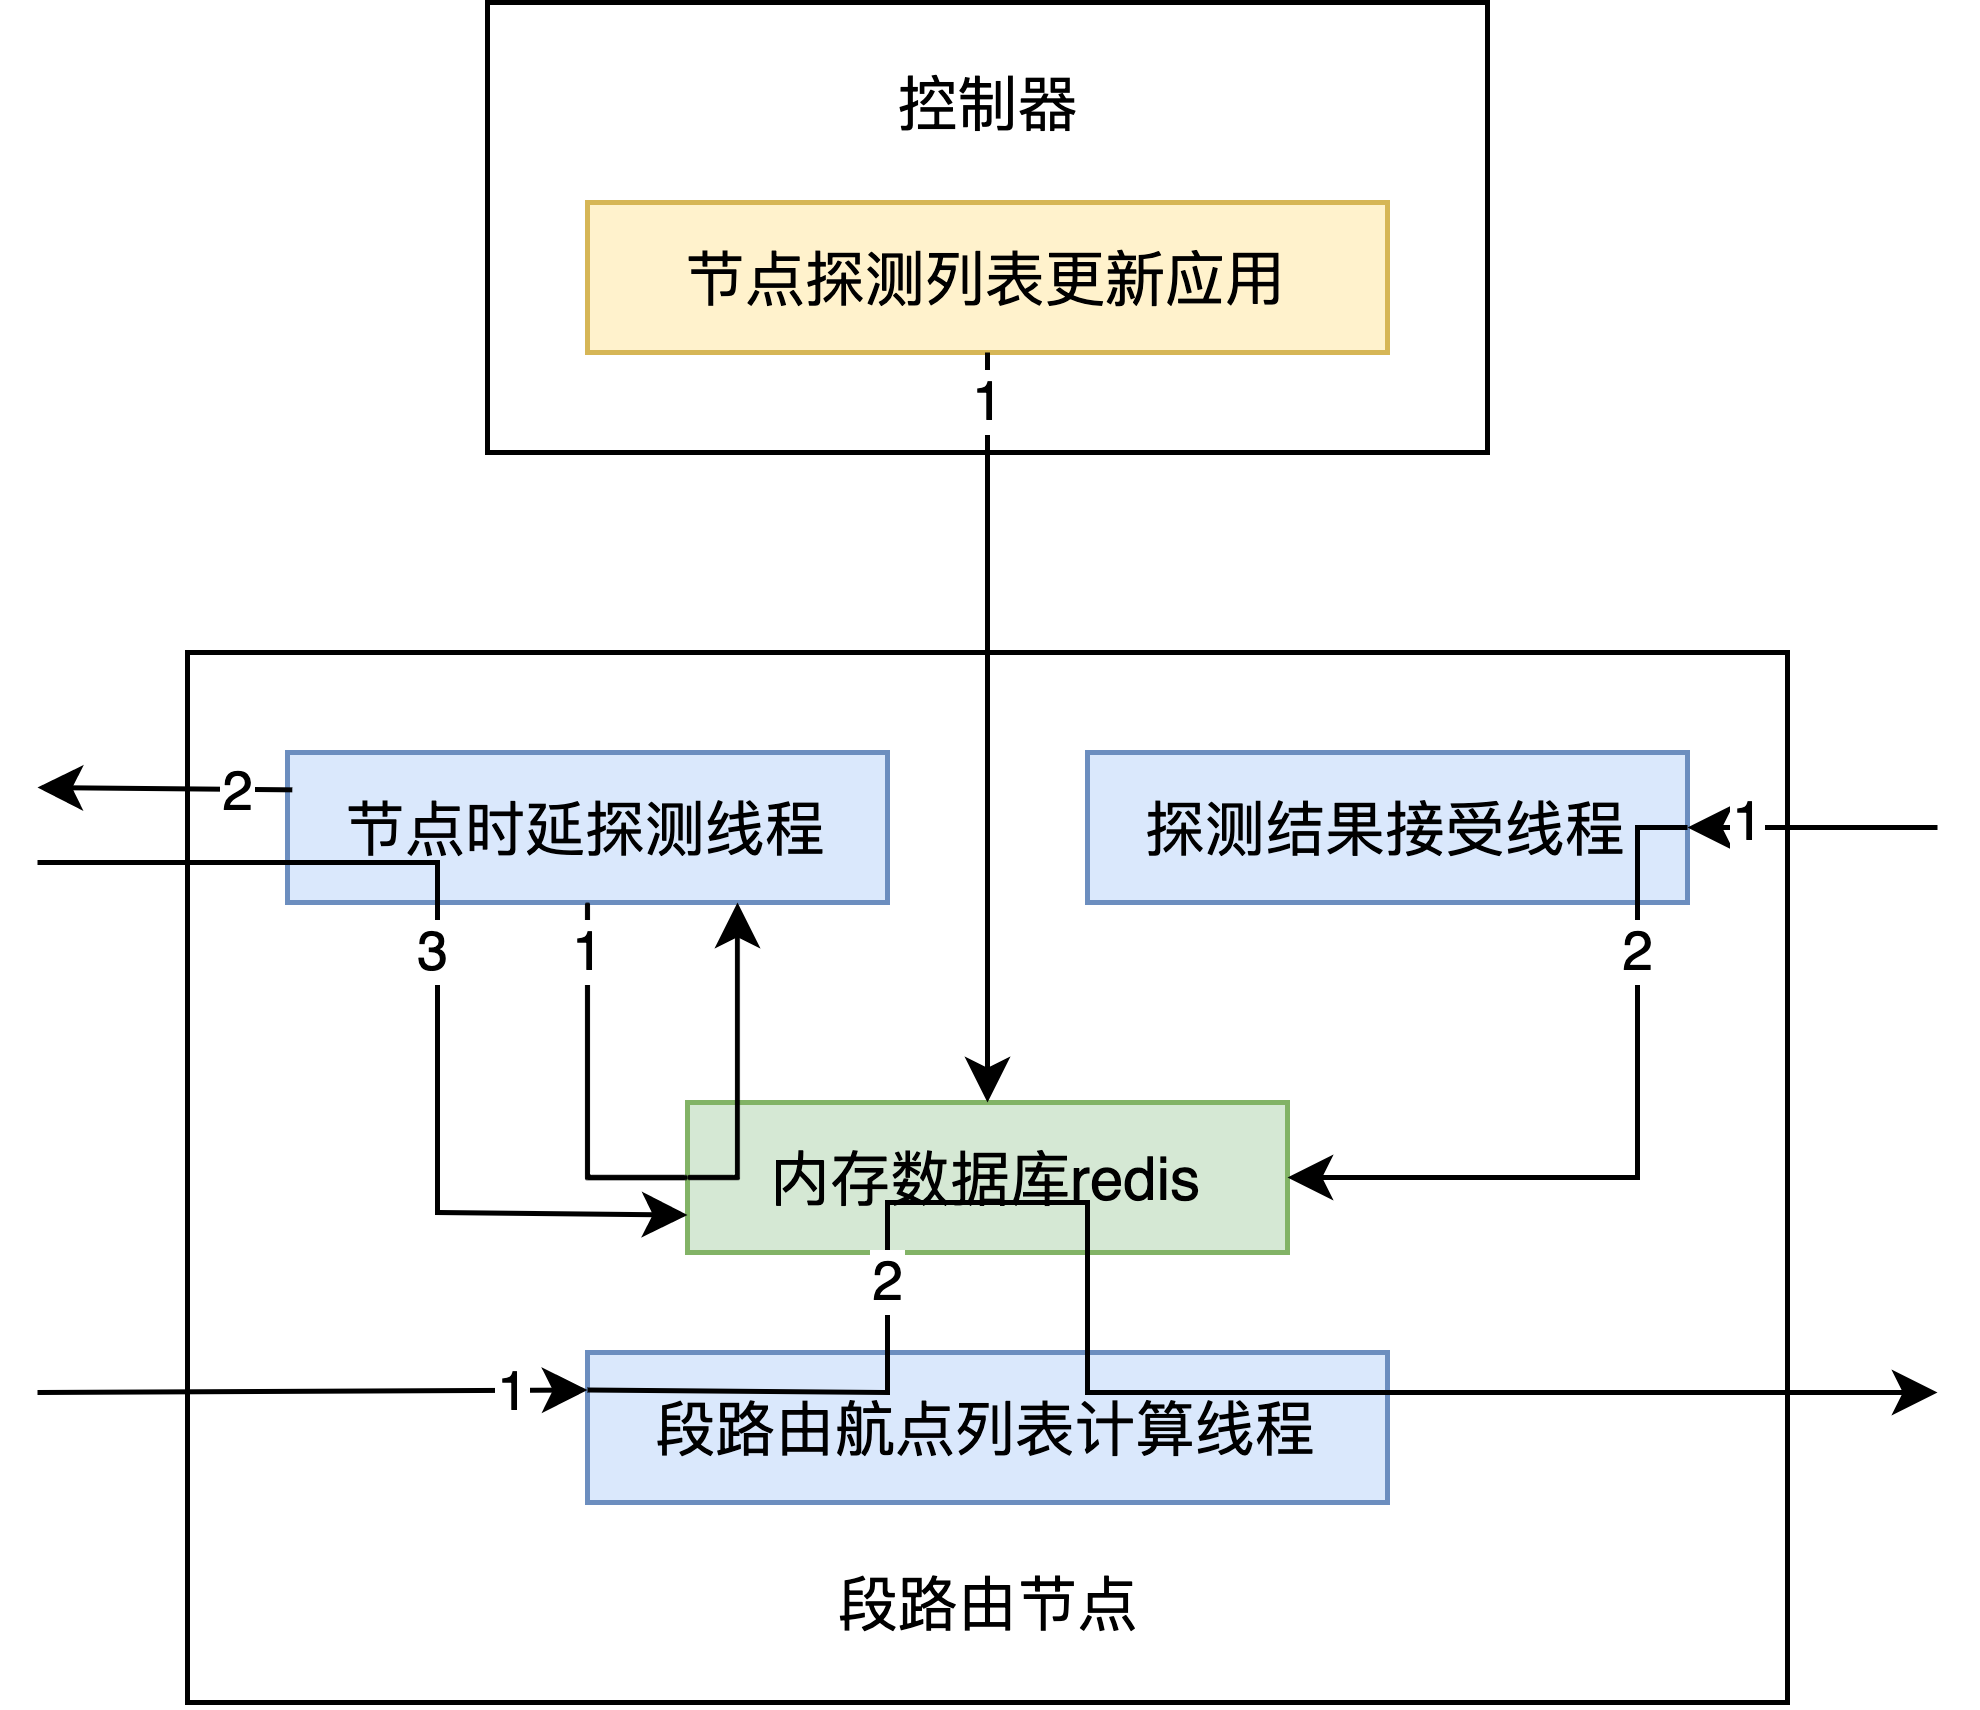
\includegraphics[width=0.8\textwidth]{./figures/ch4-test-code.png}}
\caption{实验代码结构示意图}
\label{fig-ch4-test-code}
\end{figure}
    
整个实验实现架构如图4-10所示:节点时延探测线程由计时器触发,第一步从内存数据库中获取需要进行时延探测的节点列表,第二步对外进行时延探测并记录结果,第三步将采集的结果与内存数据库中的差分时延矩阵数据进行比较并按照更新算法进行更新。探测结果接收线程由本节点的公告报文嗅探机制接收到其他段路由节点发送来的报文这一事件触发,第一步接收公告报文并处理报文内容,第二步将发布节点公告的时延的信息按照实验矩阵更新算法在内存数据库中进行更新。段路由航点列表计算线程由本节点的业务报文嗅探机制接收到带有目标时延请求的报文这一事件触发,第一步接受业务报文并提取目标地址和目标时延,第二步通过段路由航点列表生成算法生成段路由航点列表。

本文使用两种不同的段路由节点拓扑结构来评估基于差分时延的路径选择算法。数据中心拓扑由树状拓扑通过调惨生成,运营商网络通过随机网络生成,本文将通过调节拓扑的节点数来逐步验证本章提出的分布式段路由航点生成算法。

2. 实验流量

本章同第三章一样,仍然采用流量生成软件Iperf进行流量生成。主要发送TCP流量,这是为了获取报文中详细信息的时间戳,来对算法的时延保障效果进行比对。

3. 对比方案

本章算法实验的对比方案主要有自我对比和与其他路由算法进行对比,自我对比的对照组是是否选择对段路由航点列表长度进行限制以及限制的长度;其他路由算法主要是基于最短路径原理的开放最短路径优先协议和边界网关协议,实验主要利用开放最短路径优先对比本章提出算法的实际使用下端到端的总跳数,主要利用边界网关协议比较本章提出算法对时延需求的保障效果。

\subsection{实验步骤}

实验步骤分为单点算法资源消耗对比实验步骤和网络时延保障实验步骤。

第一步启动网络拓扑,新建容器,每一个容器相当于一个段路由节点,每个容器中运行模拟边界网关协议的自由范围路由进程或者运行本章提出的算法实现进程。将虚拟以太网的两端分别绑定到对应的容器分配的端口上并分配IPv6地址,启动开放最短路径优先应用生成基本路由表,这样在每对虚拟以太网间就形成连接两个虚拟交换机的链路。

第二步将设计好的拓扑中的每个段路由节点中的算法进程启动,控制应用将初始化内存数据库中每个节点的时延探测列表,段路由节点中的探测结果接收线程和段路由航点列表计算线程将开始监听各个绑定虚拟以太网的端口嗅探公告时延数据包和服务请求数据包。

第三步在网络中选择两组相隔较远的段路由节点容器,开始用流量生成软件Iperf持续性打流,保证网络运行在有基础流量的动态环境下。

第四步调整分布式段路由航点选择算法参数,例如选择限制段路由列表长度还是不限制段路由列表长度,调整惩罚值半衰期的时间等参数。

第五步选择一个源节点和目的节点开始从小流量开始打流,直到开始发生大规模的丢包,记录每次增加流量后两端航点端到端的时延情况。

第六步分析整理数据,得出结论。

\subsection{实验结果}

\begin{figure}[htbp]
\setlength{\abovecaptionskip}{15pt plus 3pt minus 2pt}
\centerline{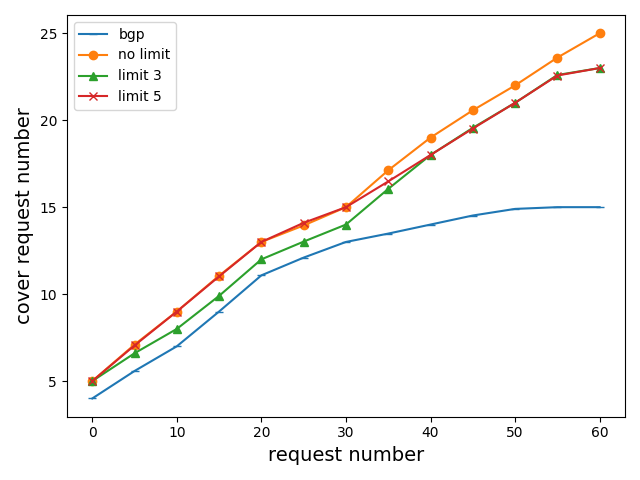
\includegraphics[width=0.8\textwidth]{./figures/ch4-test-tree-topo.png}}
\caption{树状拓扑下与边界网关协议对时延需求保障的比较结果图}
\label{fig-ch4-test-tree-topo}
\end{figure}

\begin{figure}[htbp]
\setlength{\abovecaptionskip}{15pt plus 3pt minus 2pt}
\centerline{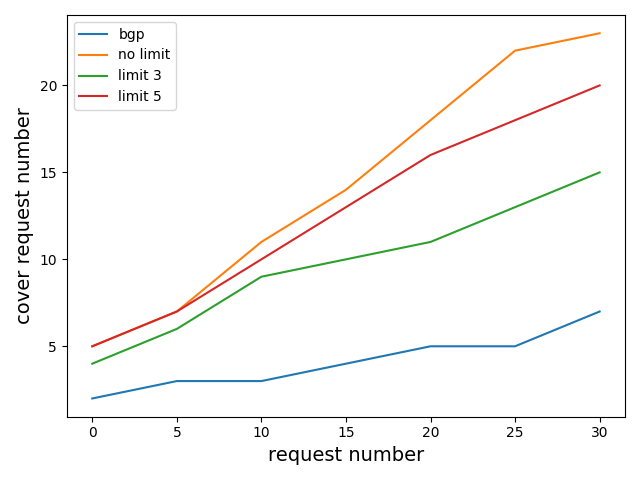
\includegraphics[width=0.8\textwidth]{./figures/ch4-test-random-topo.png}}
\caption{随机拓扑下与边界网关协议对时延需求保障的比较结果图}
\label{fig-ch4-test-random-topo}
\end{figure}

\begin{figure}[htbp]
\setlength{\abovecaptionskip}{15pt plus 3pt minus 2pt}
\centerline{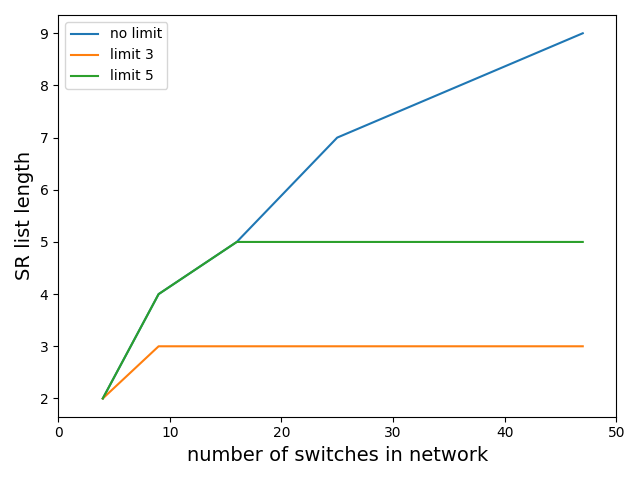
\includegraphics[width=0.8\textwidth]{./figures/ch4-sl-length.png}}
\caption{段路由标签列表长度分布结果图}
\label{fig-ch4-sl-length}
\end{figure}

\begin{figure}[htbp]
\setlength{\abovecaptionskip}{15pt plus 3pt minus 2pt}
\centerline{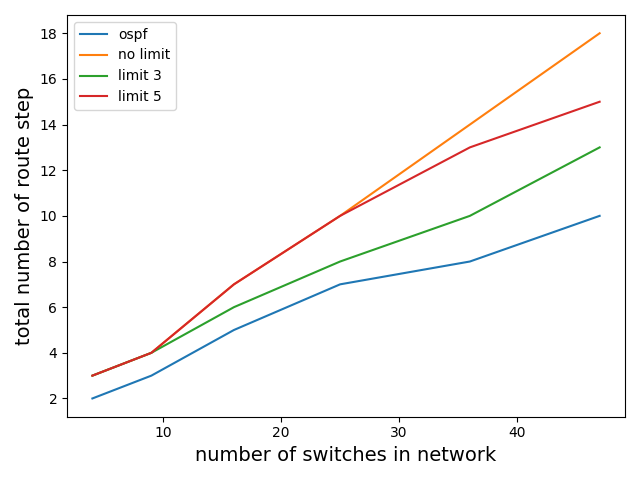
\includegraphics[width=0.8\textwidth]{./figures/ch4-total-length.png}}
\caption{基于差分时延的路径选择算法和最短路径算法的跳数对比结果图}
\label{fig-ch4-total-length}
\end{figure}
                
1. 树状拓扑下与边界网关协议对时延需求保障的比较

本实验是为了验证在同样使用数据中心树状拓扑的前提下,采用本章提出的保障时延的分布式段路由航点标签列表生成算法是否比边界网关协议有更好的时延需求保障能力。在第三章提到的算法中分析了段路由列表太长会带来的问题,并且建议不要使用过长的段路由列表,而在本章的算法中,具有对段路由标签长度进行限制和不进行限制的两种可选项,因此本实验将测试对段路由标签列表长度进行限制是否会大幅度影响路由调度的实验保障结果。本实验的自变量是服务请求的数目,这些服务请求到达时会携带一个期望的时延需求,因此用服务请求数目做为横坐标,因变量是可以满足时延需求的请求的数目,并将其在纵坐标上描点。本实验的对照组为运行边界网关协议和运行不限制标签列表长度的本章算法下,流量对时延结果的保障情况。分析实验结果数据可以初步得出结论:本章提出的分布式段路由航点标签列表生成算法确实比平常使用的分布式协议更能较好地保障业务的时延需求,段路由标签列表长度限制在3的时候,也可以达到较好的时延保障效果。

2. 随机拓扑下与边界网关协议对时延需求保障的比较

本实验与实验2类似,区别是将实验拓扑设置为模拟运营商网络的随机拓扑。本实验的自变量是在随机网络拓扑中携带目标时延发起服务请求的请求数目,并用该服务请求数目做为横坐标,纵坐标为可以满足其对应时延需求的服务请求的数目。本实验的对照组为运行边界网关协议和运行不限制标签列表长度的本章算法下,流量对时延结果的保障情况。通过分析实验结论数据可以得出结论,本章提出的分布式段路由航点标签列表生成算法在模拟运营商网络的随机网络拓扑中也能比其他路由协议更好地保障业务流量的时延需求,而段路由标签列表长度限制在5的时候,也可以达到和不限制下相当的较好的时延保障效果。

3. 基于差分时延的路径选择算法对段路由标签列表长度分布

当不对段路由标签列表长度进行限制的情况下,本章算法生成的段路由标签列表长度会因网络规模的扩大而增加,因此本实验主要是验证算法生成的段路由标签列表长度随着网络规模的扩大会呈现怎样的分布。本实验自变量时网络中段路由节点的数目,纵坐标因变量则是10个服务请求下计算出段路由航点列表的平均长度,对照组有对标签列表长度进行限制的算法结果段路由航点列表的平均长度。由实验结果可以看出,在不加限制的情况下段路由标签列表会和网络拓扑大小基本成线性增长,而限制段路由航点列表长度则会将标签列表长度固定,因此得出结论本算法需要根据具体网络拓扑情况,在生成段路由标签列表的时候对列表长度进行限制。

4. 基于差分时延的路径选择算法和最短路径算法的跳数对比

本实验目的是对比本章提出算法的流量路径跳数是否过高,因为跳数过多会对网络带来较大的额外带宽开销,本实验自变量是网络中总节点的数目,因变量是报文在本章段路由航点列表生成算法得到的段路由列表指导下平均总跳数,对照组时同样拓扑和同样流量服务需求下,按照开放最短路径优先协议进行流量转发最终经历的总跳数的平均值。由实验结果可以看出,在不加限制的情况下段路由标签列表指导下的路由跳数会和网络拓扑直径大小基本成线性增长,并且总跳数比开放最短路径优先协议多4.7\%到23.5\%,而开放最短路径优先协议下的总跳数总是基本和网络直径相当。

\section{算法结论}

本文提出了一种分布式的段路由航点列表生成算法,用于在网络节点较多的广域网络中用分布式的方式提供基于段路由的低延迟路径流量调度服务。由于本章主要采用分布式,因此缺少了软件定义网络下控制器集中式的网络优化途径,但也正因为没有使用集中式控制器使得本章提出的算法可以较为简单地在更大的网络内直接部署。本章算法的核心在于差分时延矩阵的生成、更新和选择,本章对算法进行了详细的解释,并留出了一些参数可以在实验或者真实场景部署阶段进行调整,例如惩罚值的压制阈值等。最后本章通过实验验证了该段路由航点列表生成算法生成的短路有策略是可以有效保障流量需求时延的。并且对数据中心拓扑和运营商拓扑分别适合的段路由标签列表长度进行了测试,最终本算法要求在使用时根据拓扑的情况配置段路由航点列表的长度限制,这是为了防止过长的段路由航点列表造成较低的链路有效负载和造成过多的端到端总跳数降低整个网络的吞吐量。

% \chapter{基于P4的算法实验验证}

% \section{引言}

% \section{实验环境}

% \section{基础实验}

% \section{组网实验}

% \section{算法结论}

% 测试所有参考文献类型\cite{CITATION_BOOK,CITATION_ARTICLE,CITATION_PROCEEDINGS,CITATION_INPROCEEDINGS,CITATION_TECHREPORT,CITATION_STANDARD,CITATION_PATENT,CITATION_NEWSPAPER,CITATION_ELECTRONIC,SRSURVEYS}。

%% 本章参考文献
\ifx\usechapbib\empty
\nocite{BSTcontrol}
\setcounter{NAT@ctr}{0}
\bibliographystyle{buptgraduatethesis}
\bibliography{bare_thesis}
\fi


\ifx\usechapbib\undefined
\bibliographystyle{buptgraduatethesis}
\bibliography{bare_thesis}
\fi

%% 附录部分

%% 如果有两个或两个以上的附录, 使用appendix环境
\begin{appendix}
  %%
%% This is file `example/app_lhospital.tex',
%% generated with the docstrip utility.
%%
%% The original source files were:
%%
%% install/buptgraduatethesis.dtx  (with options: `app-lhospital')
%% 
%% This file is a part of the example of BUPTGraduateThesis.
%% 

\chapter{不定型($0/0$)极限的计算}
\begin{theorem}[L'Hospital法则]
  若
  \begin{enumerate}
  \item 当 $x \to a$ 时,函数 $f(x)$ 和 $g(x)$ 都趋于零;
  \item 在点 $a$ 某去心邻域内,$f'(x)$ 和 $g'(x)$ 都存在,且 $g'(x)\neq 0$;
  \item $\displaystyle\lim_{x \to a} \dfrac{f'(x)}{g'(x)}$ 存在(或为无穷大),
  \end{enumerate}
  那么
  \begin{align}
    \label{eq:app:lhospital}
    \lim_{x \to a} \frac{f(x)}{g(x)} = \lim_{x \to a} \frac{f'(x)}{g'(x)}.
  \end{align}
\end{theorem}
\begin{proof}
  以下只证明两函数 $f(x)$ 和 $g(x)$ 在 $x = a$ 为光滑函数的情形。
  由于 $f(a) = g(a) = 0$,原极限可以重写为
  \begin{align*}
    \lim_{x \to a} \frac{f(x) - f(a)}{g(x) - g(a)}.
  \end{align*}
  对分子分母同时除以 $(x - a)$,得到
  \begin{align*}
    \lim_{x \to a} \frac{%
      \dfrac{f(x) - f(a)}{x - a}
    }{%
      \dfrac{g(x) - g(a)}{x - a}
    } &
    = \frac{%
      \displaystyle\lim_{x \to a} \frac{f(x) - f(a)}{x - a}
    }{%
      \displaystyle\lim_{x \to a} \frac{g(x) - g(a)}{x - a}
    }.
  \end{align*}
  分子分母各得一差商极限,即函数 $f(x)$ 和 $g(x)$ 分别在 $x = a$ 处的导数
  \begin{align*}
    \lim_{x \to a} \frac{f(x)}{g(x)} &
    = \frac{f'(a)}{g'(a)}.
  \end{align*}
  由光滑函数的导函数必为一光滑函数,故 \eqref{eq:app:lhospital} 得证。
\end{proof}

  % 自动抽取生成缩略语表作为附录A
  \tableofacronyms
  % 用\input{}添加其他的附录
  % \input{...}
\end{appendix}

%% 如果只有一个附录, 使用appendix*环境
%% \begin{appendix*}
%%   % 自动抽取生成缩略语表作为附录A
%%   % \tableofacronyms
%% \end{appendix*}

\backmatter
%% 致谢
\ifx\ispeerreview\undefined
%%
%% This is file `example/ackgmt.tex',
%% generated with the docstrip utility.
%%
%% The original source files were:
%%
%% install/buptgraduatethesis.dtx  (with options: `ackgmt')
%% 
%% This file is a part of the example of BUPTGraduateThesis.
%% 

\begin{acknowledgement}
  %% 感谢所有你应该感谢的人
  % 感谢Donald Ervin Knuth.
  光阴似箭,日月如梭,转眼间我已经即将完成三年在北京邮电大学的硕士生涯。回首过来我确实有太多的人要感谢。

  首先要感谢我的导师杨帆,是杨老师以极其包容的态度让我在实验室的一年研零和三年研究生中学习体会网络的魅力,并深深影响我求职道路上的选择。

  其次要感谢我同级的好朋友崔明玮和谢雅琼,我们一起合作写文档,一起分工写代码,一起出差一起交接项目,有你们两人的陪伴和合作,我的研究生生活非常快乐。还有其他实验室的同学和老师,先我毕业的师兄师姐、即将后我毕业的师弟师妹,当然还有同级的好友们,魏浩然、顾笛儿、康洁、张馨元,刘克非...想起你们的相处我都会觉得十分温暖。

  再者我需要感谢我研究生的舍友们,常梦迪、陈泓宇、李逸潇、王玉铭、杨雪莹(按照首字母排序),是你们在每一个熬夜学习的晚上为我提供支持,在备考和求职的路上守望相助,在我一个人在学校度过的春节里给我邮寄家乡的美食,因为有你们,我的研究生生活是那样的丰富多彩。

  除了研究生的舍友,我当然不能忘记我本科的好舍友们。感谢李聪、谭莉、张晗、张钧懿(按照首字母排序),你们是我坚持强的后盾,是我在学校生活之外港湾,是督促我前进的动力。

  我感谢学校、感谢导员、感谢班委、感谢食堂的工作人员、感谢楼管阿姨、感谢常驻学校的快递小哥...这些生活在我周围的人是我学校生活的保障。
  
  我感谢字节跳动的同学在我实习期间的信任和照顾,在我下定决心继续在网络领域的工作上影响颇深。

  当然还有我的家人们,感谢我的父亲母亲外公还有好几个舅舅,他们从不担心我的学习和工作,只担心我的身体,他们永远怕我太累时常让我照顾好自己,常常给我寄来家里的水果干果,祝福我健康顺利。

  最后我还要感谢我亲爱的不愿透露姓名的男朋友,我2022年的春节留在了北京,留在了学校过年,这是我最艰难的一段时间,是你每天陪我电话给我支持,给我鼓励,让我顺利完成了论文。

  我想可能很少有人写致谢写这么多人名,但是我翻了翻我的通讯录,让我心怀感动需要感谢实在是太多了,我为我这一段研究生岁月能顺利毕业而骄傲,也为我能碰见这样多的贵人而自豪。在即将毕业的时候我也希望未来能将我在研究生深造的知识和能力造福更多的人、建设更好的网络、建设更好的国家。

\end{acknowledgement}

\fi

%% 在读期间论文发表情况
%%
%% This is file `example/pubs.tex',
%% generated with the docstrip utility.
%%
%% The original source files were:
%%
%% install/buptgraduatethesis.dtx  (with options: `pubs')
%% 
%% This file is a part of the example of BUPTGraduateThesis.
%% 

%% 发表论文列表

%% 攻读学位期间发表论文列表用 tableofpublications 环境产生。需要
%% 在 bare_thesis.tex 的导言区用 \newcite{<name>}{<caption>} 声明不同类
%% 型的论文,具体见导言区说明。
%% 根据各类论文发表数量设置\setbiblabelwidth{<num>},用于控制发表论文序号的对齐位置。
%% 例如:发表conf类论文数量为个位数,则<num>=1;发表jrnl类论文数量为两位数,则<num>=10;
\begin{tableofpublications}
  \thispagestyle{bupt@pubheadings}%
  \setcounter{NAT@ctr}{0}
  \setbiblabelwidth{1}
  \bibliographyjrnl{pubs}
  \nocitejrnl{LAILIRONG}

  % \setbiblabelwidth{1}
  % \bibliographyconf{pubs}
  % \nociteconf{paper2}

  % \setbiblabelwidth{1}
  % \bibliographypatent{pubs}
  % \nocitepatent{patent1}
\end{tableofpublications}


\newpage
\end{document}
